\chapter{Why use Statistical Models?}
\label{sec:ch5}

At the foundation of statistical inference is the statistical model. This concept can seem somewhat esoteric, and often times, the word "statistical model", we find, is a bit overused. However, it is extremely important to clarify exactly what a statistical model is, and what it isn't, so we hope to clear up some of those misconceptions here before we jump in. A statistical model is, at its core, {purely theoretical} in nature. Statistical models fit into the network learning pipeline like in Figure \ref{fig:ch5:netmodels}:
\begin{figure}[h]
    \centering
    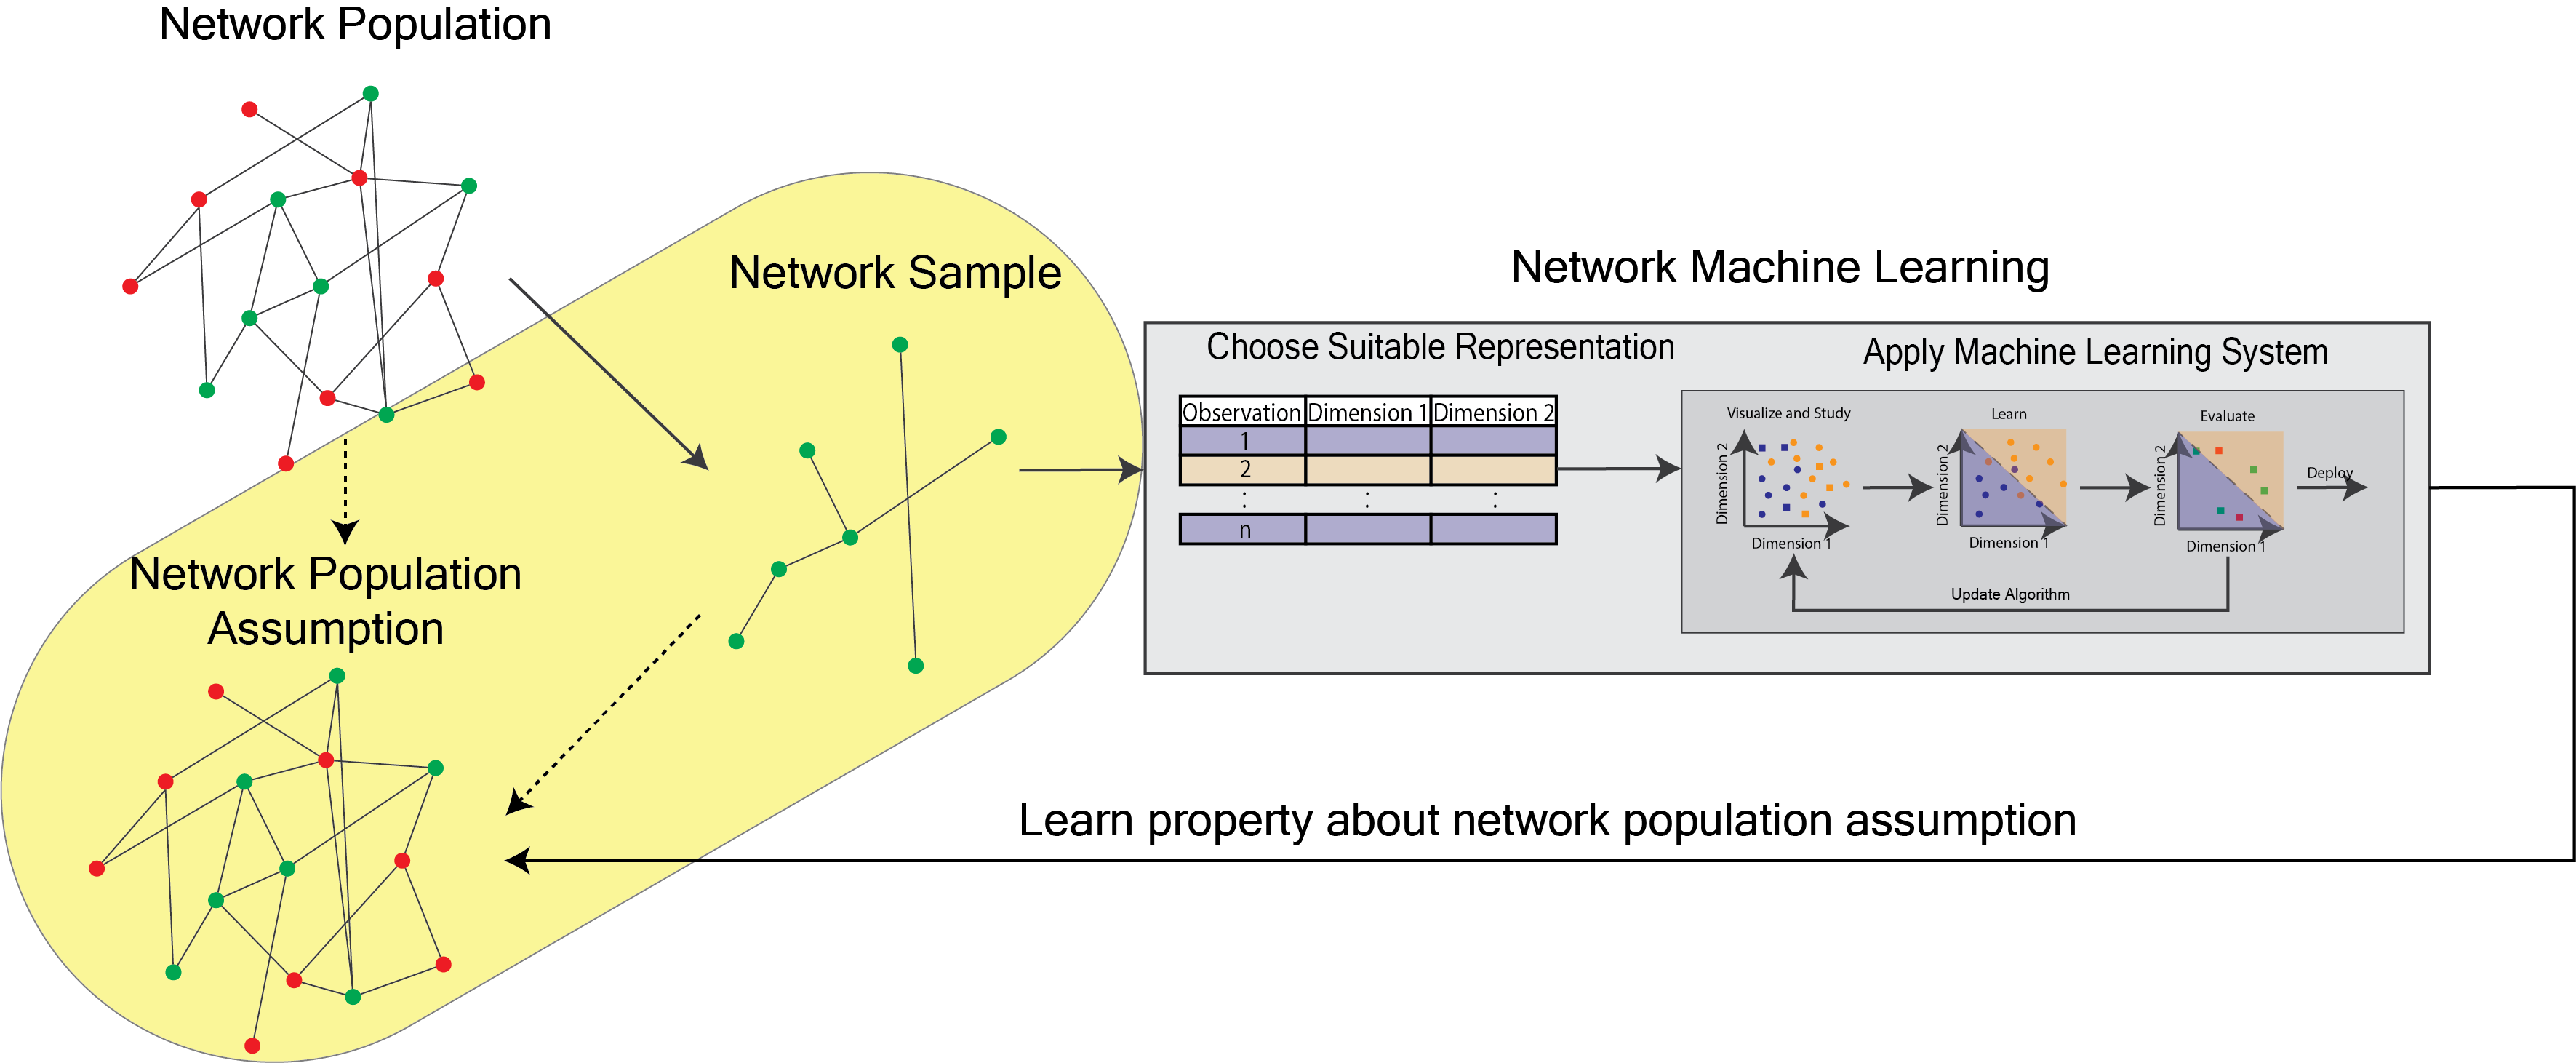
\includegraphics[width=\linewidth]{representations/ch5/Images/network_modelling.png}
    \caption[Network modelling schematic]{In this chapter, you will learn how to construct sets of assumptions about the network which underlies your network sample.}
    \label{fig:ch5:netmodels}
\end{figure}

The reality is, the network you observe, which you learned how to describe in the previous chapter, is not {typically} the thing you want to learn about. Rather, you want to learn about the {system} which underlies the network you observed. To learn about the dynamics of this system is a three-step process: first, you need to assume some things about the system (this chapter); second, you need to learn representations of the network you see that will be useful to you (the next chapter), and finally, you need to learn how that representation can inform the assumptions you made about the system. This process can be boiled down quite a bit to how flipping a coin works. When you flip a coin, usually you don't know ahead of time whether that coin is going to land on heads or tails. Instead, you think that coin is going to land on heads or tails with some probability (usually, an even chance of landing on heads or tails, or a probability of $0.5$). If you flip the coin once and get heads, you don't think that coin is {only} going to ever land on heads: rather, you think that coin landed on heads because of some amount of random chance. 

And herein, you just assumed a statistical model. You assumed that the outcome of your coin (the random object, here, that you are modelling) was heads or tails with some probability, and when you saw that outcome (the {sample} of the coin flip) you prescribed that outcome to one of the possible outcomes occurring. As you'll see briefly, network modelling is nearly the same, and for simple networks especially, is {almost exactly} the same as flipping coins. Throughout this chapter, you'll learn to think about each edge of the network as a particular coin. Remember that the edges for a simple (and consequently, {unweighted}) network either exist or they don't exist: this is exactly like a coin landing on heads or tails. The key difference is that the edges existing or not existing might happen at probabilities different from $0.5$; there might be a chance of $0.7$ that one edge exists, or $0.4$ that another edge exists. 

When you construct models for networks, what you are going to do is prescribe sets of assumptions for how the coin for each edge behaves: are all of the edges in the network flipping coins with equal probability (do all the edges exist or not exist with the same chance)? Are there some groups of nodes whose edges all have the same probabilities? Are there other ways you can describe the probabilities that other edges exist or do not exist? 

\begin{comment}
We'll learn about the following models, which tend to be some of the more common simple network models for network learning:

\begin{enumerate}
    \item Section \ref{sec:ch5:er} covers the Erd\"os-R\'enyi (ER) random network, which is the simplest model for network data.
    \item Section \ref{sec:ch5:sbm} covers the Stochastic Block Model (SBM), which is a model for network data that conveys community structure.
    \item Section \ref{sec:ch5:rdpg} covers the Random Dot Product Graph (RDPG), which is a model which we will use later to conceptualize techniques to learn representations of network data.
    \item Section \ref{sec:ch5:ier} covers the Inhomogeneous Erd\"os R\'enyi (IER) random network, which is the most complicated independent-edge network model.
    \item Section \ref{sec:ch5:dcsbm} covers the degree-corrected SBM (DCSBM), which is an augmentation of the SBM that allows for some nodes to be more (or less) connected than others.
    \item Section \ref{sec:ch5:psd_block} covers different types of block matrices for SBMs, and when these can be conceptualized using an RDPG.
    \item Section \ref{sec:ch5:siem} covers the structured independent-edge model (SIEM), which will be used later to facilitate testing on groups of edges in the network.
    \item Section \ref{sec:ch5:multi} covers network models for when we have more than one network.
    \item Section \ref{sec:ch5:multicovar} covers the signal subnetwork (SSN) model, a model for when we have network-specific covariates.
\end{enumerate}
\end{comment}

Network modelling can get pretty dicey in probability and statistical theory rather quickly. For this reason, for the main text of the book, we've tried to keep the level of statistical depth required as low as possible, so that you can focus more on the intuition and mathematical relationships and less on the statistical rigor. For the more technical readers, Appendix \ref{app:ch12} provides more in-depth coverage of statistical network models.

\newpage

\section{Erd\"os-R\'enyi Random Networks}
\label{sec:ch5:er}


We will start to learn about random networks with the simplest random network model. Consider a social network, with 50 students. Our network will have 50 nodes, where each node represents a single student in the network. Edges in the social network represent whether or not a pair of students are friends. What is the simplest way you could describe whether two people are friends?

In network machine learning, you get to see an adjacency matrix $A$ whose entries $a_{ij}$ are one if the students $i$ and $j$ are friends on the social networking site, and $0$ if the students $i$ and $j$ are not friends on the social networking site. You have $n$ students in total, so the adjacency matrix $A$ is going to be $n \times n$. 

\begin{floatingbox}[h]\caption{Making the leap to statistical modelling with coin flips}
When you have a coin, before you flip it, the outcome is either heads or tails, with some probability. We'll denote this coin, for which we don't know the outcome (because we haven't flipped it), by the letter $\mathbf x$. 

The best way that we can describe this coin is not by heads and tails, but rather, by {probabilities} that it lands on heads or tails. For a coin, what we'd say is that a sample $x$ (an outcome of a flip of the coin $\mathbf x$) is heads with probability $p$ or tails with probability $1-p$ (the coin can only land on heads or tails, so the probabilities must sum up to $1$). 

When specifying the statistical model, you don't make any assumptions about the probabilities; you just specify that they are probabilities, and leave it at that. For a normal, {fair} coin, $p$ would be $0.5$, but we don't even want to get that specific when we come up with a statistical model for a system.
\end{floatingbox}

Now, let's rotate back to the network. Since our observation $A$ was an $n \times n$ matrix, our random variable $\mathbf A$ is an $n \times n$ random matrix. The elements of $\mathbf A$ will be given by the symbols $\mathbf a_{ij}$, which means that each edge $a_{ij}$ of $A$ is a sample of the random edge $\mathbf a_{ij}$. Just how do you describe this $\mathbf a_{ij}$? 

Remember that our samples $a_{ij}$ are just $0$s and $1$s, which {feels} a lot like flipping a coin, doesn't it? Did the coin land on heads, or did it land on tails? Are the two people $i$ and $j$ friends, or are they not friends? If you had a coin with some probability of landing on heads, you could describe $a_{ij}$ as a sample of this coin flip. You could assume that a value of one is analogous to the coin landing on heads, and value of zero is analogous to the coin landing on tails. Perhaps you could even model the network using the same approach you took before with the coin flip. This is starting to go somewhere, so let's continue with the analogies.


\subsection{The Erd\"os R\'enyi random network is parametrized by the independent-edge probability}

The simplest random network model is called the Erd\"os R\'enyi (ER) model, which was first described by \cite{erdos59a} and \cite{Gilbert1959Dec}. The way you can think of an ER random network is that the edges depend {only} on a probability, $p$, and each edge is totally independent of all other edges. You can think of this example as though a coin flip is performed, where the coin has a probability $p$ of landing on heads, and $1-p$ of landing on tails. For each edge in the network, you conceptually flip the coin, and if it lands on heads (with probability $p$), the edge exists, and if it lands on tails (with probability $1-p$) the edge does not exist. If $\mathbf A$ is a random network which is $ER_n(p)$ with $n$ nodes and probability $p$, we will say that $\mathbf A$ is an $ER_n(p)$ random network.

\begin{floatingbox}[h]\caption{What part of this is the statistical model?}
The statistical model, here, is just the description of the system. {All} of the edges of the underlying random network, $\mathbf A$, have a probability $p$ of existing or not existing. This probability is the same for all edges. The edges are independent, and whether one edge exists does not impact whether any other edges exist. 

Again, the probability is left generic in the statistical model: it is just $p$, which could be $0.5$, $0.7$, $0.4$, really just any probability (a number between $0$ and $1$). It's really as simple as that!
\end{floatingbox}


\subsection{How do you simulate samples of $ER_n(p)$ random networks?}

This approach which you will use to describe random networks is called a {generative model}, which means that you have described an observable network sample $A$ of the random network $\mathbf A$ in terms of the parameters of $\mathbf A$. In the case of the ER random networks, you have described $\mathbf A$ in terms of the probability parameter, $p$. Generative models are convenient in that you can easily adapt them to tell us exactly how to simulate samples of the underlying random network. The procedure in Algorithm \ref{alg:ch5:er} will produce for us a network $A$, which has nodes and edges, where the underlying random network $\mathbf A$ is an $ER_n(p)$ random network.

\begin{algorithm}[h]\caption{Simulating a sample from an $ER_n(p)$ random network}
\label{alg:ch5:er}
\SetAlgoLined
\KwData{$n$ a number of nodes\newline $p$ a probability of an edge existing}
\KwResult{The adjacency matrix of a sample from the random network.}

Obtain a weighted coin which has a probability $p$ of landing on heads, and a probability $1 - p$ of landing on tails. Note this probability $p$ might differ from the "traditional" coin with a probability of landing on heads of approximately $0.5$.

\For{$i$ in $1$:$n$} {
    \For{$j > i$} {
        Flip the coin once. If the coin lands on heads, let $a_{ij} = 1$. If the coin lands on tails, let $a_{ij} = 0$.

        Let $a_{ji} = a_{ij}$.
    }
}

\Return{$A$}
\end{algorithm}

\begin{floatingbox}[h]\caption{Notation and word choice regarding networks and random networks}
When you are deciding on notation that you will use for your work, it is {extremely} easy to get confused very quickly. Within this work, since we are regularly dealing with matrices, vectors, and scalar quantities, we use boldface $\mathbf A$ to denote a network which is random. 

It is important to clarify that, even if you have a network that was {generated} using a process to produce a sample of a random network, such as Algorithm \ref{alg:ch5:er}, that the adjacency matrix $A$ that you end up with is not random once you produce the sample. It is then a {realized} network sample, and it is {not} a random network anymore. 

To think about this with coin flips, before you flip the coin, the outcome is random. It will land on heads or tails with some probability. Once you flip the coin, the outcome is fully determined, and the outcome is no longer random. This notational (and wording) distinction causes a {lot} of problems for people across many scientific fields. You will see a lot of work out there where people will sample a network, giving them a collection of nodes and edges, and then assert that this network sample is random. The sample is not random at all once it is brought into existence; the mechanism that generated it was random. 
\end{floatingbox}

\subsection{When do you use an $ER_n(p)$ Network?}

In practice, the $ER_n(p)$ model seems like it might be a little too simple to be useful. Why would it ever be useful to think that the best you can do to describe our network is to say that connections exist with some probability? Does this miss a {lot} of useful questions you might want to answer? Fortunately, there are a number of ways in which the simplicity of the $ER_n(p)$ model is useful. Given a probability and a number of nodes, you can easily describe the properties you would expect to see in a network if that network were ER. For instance, you know how many edges on average the nodes of an $ER_n(p)$ random nework should have. 

You can reverse this idea, too: given a network you think might {not} be ER, you could check whether it's different in some way from an $ER_n(p)$ random network. It is often useful to start with the {simplest} random network models first when you are analyzing your network data, and only turning to more complicated network models when the need arises, because the types of network models you choose will directly determine the types of questions you can answer later on. For instance, if you see that half the nodes have a ton of edges (meaning, they have a high degree), and half don't, you might be able to determine that the network is poorly described by an $ER_n(p)$ random network. If this is the case, you might look for other models that could describe our network which are more complex. 

In the next code block, we are going to sample a single $ER_n(p)$ network with $50$ nodes and an edge probability $p$ of $0.3$:


\begin{lstlisting}[style=python]
from graphbook_code import draw_multiplot
from graspologic.simulations import er_np

n = 50  # network with 50 nodes
p = 0.3  # probability of an edge existing is .3

# sample a single simple adjacency matrix from ER(50, .3)
A = er_np(n=n, p=p, directed=False, loops=False)

# and plot it
draw_multiplot(A.astype(int), title="$ER_{50}(0.3)$ Simulation")
\end{lstlisting}
Our visualization is a heatmap and layout plot like you learned in Section \ref{sec:ch4:mtx-rep}. The heatmap is shown in Figure \ref{fig:ch5:er}(A).

\begin{figure}
    \centering
    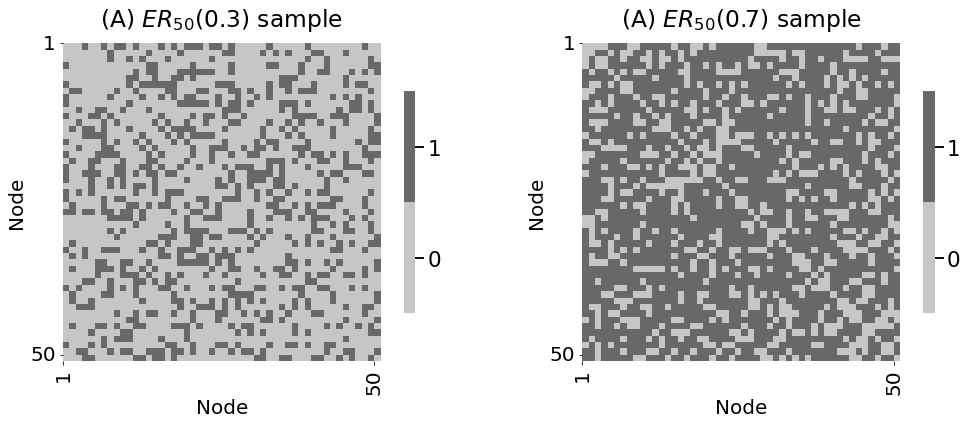
\includegraphics[width=\linewidth]{representations/ch5/Images/er.png}
    \caption[A sample from an $ER_n(p)$ network.]{\textbf{(A)} a sample with $p=0.3$. \textbf{(B)} a sample with $p=0.7$. Notice that with higher probabilities, the samples from the random network have more edges.}
    \label{fig:ch5:er}
\end{figure}

Next, let's see what happens when you use a higher edge probability, like $p=0.7$:

\begin{lstlisting}[style=python]
p = 0.7  # network has an edge probability of 0.7

# sample a single adjacency matrix from ER(50, 0.7)
A = er_np(n=n, p=p, directed=False, loops=False)
\end{lstlisting}

We show the same plot for $p=0.7$ in Figure \ref{fig:ch5:er}(B). As the edge probability increases, the sampled adjacency matrix tends to indicate that there are more connections in the network. This is because there is a higher chance of an edge existing when $p$ is larger. Correspondingly, the network density (which you learned in Section \ref{sec:ch4:prop-net:density}) increases, and the network samples tend to be more dense.

\subsection{Just how many networks are possible for a network with $n$ nodes?}
 
As you're going to become accustomed to, we're going to boil this down again to coin flips. If you had one coin, there are two possible outcomes: either heads or tails. If you had two coins, the first coin could be heads or tails, and the second coin could be heads or tails. Let's break this down by fixing the outcome of the first coin. If the first coin were heads, there are two possible outcomes for the second coin. If the first coin were tails, there are two possible outcomes for the second coin. This means that the total number of possible outcomes is the sum of the number of possible outcomes if the first coin is heads with the number of possible outcomes if the first coin were tails. This gives us that with two coins, you have four possible outcomes. When you add a third coin, you repeat this process again. If the first coin were heads, the second two coins could take any of four possible outcomes as you just learned. if the first coin were tails, the second two coins could also take any of four possible outcomes. Therefore, with three coins, you have eight possible outcomes. As you continue this procedure, you quickly will realize that with $x$ coin flips, you have $2^x$ possible outcomes. 

Remember in Section \ref{sec:ch4:prop-net:density} when we were discussing the number of possible edges in a network, we determined that there are $\frac{1}{2}n(n - 1)$ possible edges in a simple network, which we could represent using the notation $\binom n 2$. In a realized network, each of these edges could exist or not exist, so there are again two possibilities just like the coin flips. Since edges existing or not existing boils down to a coin flip, the number of possible networks with $n$ nodes is just $2$ to the power of the number of coin flips that are performed in the network. 

Here, this is $2^{\binom n 2}$. This quantity gets {really} big {really} fast! In the code below, we calculate the number of possible networks for a given number of nodes in a network, but as powers of $10$. This corresponds to the plot that you explored in Figure \ref{fig:ch4:nnets}.


\begin{lstlisting}[style=python]
import numpy as np
from math import comb

node_count = np.arange(2, 51)
potential_network_count = np.array([comb(n, 2) for n in node_count])*np.log10(2)
\end{lstlisting}

This is an enormous quantity! When $n$, the node count, is just $6$, the number of possible networks is $2^{\binom 6 2} = 2^{6}$ which is over $32,000$. When $n$ is $15$, the number of possible networks balloons up to $2^{\binom{15}{2}} = 2^{105}$ which is over $10^{30}$.

\begin{floatingbox}[h]\caption{So, why do we use the statistical models?}
\label{box:ch5:whyuse}
We use statistical models because describing each possible observable network for a given number of nodes is {impossible}, for two reasons:
\begin{enumerate}
    \item We could not possibly use a network with $n$ nodes that we obtain to learn things about every possible network with $n$ nodes, because our network is just one of many. If you flipped a coin once and obtained a result of heads, would you say you are extremely confident that the coin will never lands on tails? This is the same problem we have with have with network data when we do not have a sufficiently straightforward model.
    \item Even if we had more network samples, we could not possibly analyze nor even store this many possibilities, because for even modest choices of $n$, it is simply too many elements to keep track of.
\end{enumerate}
These aspects are detailed at length in Appendix \ref{app:ch12:foundation}.
\end{floatingbox}

\subsection{Read on for more}

Appendix \ref{app:ch12:ers} covers the Erd\"os R\'enyi Random Network in more technical depth. If you have a background in statistics, we would recommend that you check it out.

\newpage
\section{Stochastic Block Models}
\label{sec:ch5:sbm}

Let's imagine that you have $100$ students, each of whom can go to one of two possible schools: school one or school two. Your network has $100$ nodes, and each node represents a single student. The edges of this network represent whether a pair of students are friends. Intuitively, if two students go to the same school, the probably have a higher chance of being friends than if they do not go to the same school. If you were to try to characterize this using an ER random network, you would run into a problem: you have no way to capture the impact that school has on friendships. To do this, you need to build upon your $ER_n(p)$ model to make things a little more complicated.

The Stochastic Block Model, or SBM, captures this idea by assigning each of the $n$ nodes in the network to one of $K$ communities, and was first introduced by \cite{Holland1983Jun}. A \textit{community} is a group of nodes within the network which have similar properties. In your example case, the communities would represent the schools that students are able to attend. We use $K$ here to just denote an integer greater than $1$ (for example, in the school example we gave above, $K$ is $2$) for the number of {possible} communities that nodes could be members of. In an SBM, instead of describing all pairs of nodes with a fixed probability like with the ER model, you instead describe properties that hold for edges between {pairs of communities}. In your example, what this means is that if two students go to school one, the probability that they are friends might be different than if the two students went to school two, or if one student went to school one and the other to school two.

% \subsection{Defining the SBM random network}
\subsection{The community assignment vector assigns nodes in the random network to communities}

To describe an SBM random network, we proceed very similarly to an ER random network, with a twist. An SBM random network has a parameter, $\vec z$, which has a single element for each of the nodes. We call $\vec z$ the \textit{community assignment vector}, which means that for each node of your random network, $z_i$ tells you which community the node is in. To state this another way, $\vec z$ is a vector where each element $z_i$ can take one of $K$ possible values, where $K$ is the total number of communities in the network. For example, if you had an SBM random network with four nodes in total, and two total communities, each element $z_i$ can be either $1$ or $2$. If the first two nodes were in community $1$, and the second two in community $2$, you would say that $z_1 = 1$, $z_2 = 1$, $z_3 = 2$, and $z_4 = 2$, which means that $\vec z$ looks like:

\begin{align*}
    \vec z &= \begin{bmatrix}1 \\ 1 \\ 2 \\ 2\end{bmatrix}
\end{align*}
\subsection{The block matrix defines the edge existence probabilities between communities in the random network}

The other parameter for an SBM random network is called the block matrix, for which we will use the capital letter $B$. If there are $K$ communities in the SBM random network, then $B$ is a $K \times K$ matrix, with one entry for each pair of communities. For instance, if $K$ were two like above, $B$ would be a $2 \times 2$ matrix, and would look like this:
\begin{align*}
    B &= \begin{bmatrix}
        b_{11} & b_{12} \\ b_{21} & b_{22}
    \end{bmatrix}
\end{align*}
Each of the entries of $B$, which we denote as $b_{kl}$ in the above matrix, is a probability of an edge existing between a node in community $k$ and a node in community $l$. 

\subsection{Conceptualizing the SBM}

Fortunately, you can also think of this formulation of a random network using coin flips. In your mini example above, if node $1$ is in community $1$ (since $z_1 = 1$) and node $2$ is in community $1$ (since $z_2 = 1$), you have a weighted coin which has a probability $b_{11}$ (the first row, first column of the block matrix above) of landing on heads, and a $1 - b_{11}$ chance of landing on tails. An edge between nodes one and two exists if the weighted coin lands on heads, and does not exist if that weighted coin lands on tails. If you wanted to describe an edge between nodes one and three instead, note that $z_3 = 2$. Therefore, you use the entry $b_{12}$ as the probability of obtaining a heads for the weighted coin you flip this time. In the general case, to use the block matrix to obtain the probability of an edge $(i, j)$ existing between any pair of nodes $i$ and $j$, you will flip a coin with probability $b_{z_i z_j}$, where $z_i$ is the community assignment for the $i^{th}$ node and $z_j$ is the community assignment for the $j^{th}$ node.

If $\mathbf A$ is an SBM random network with $n$ nodes, the community vector $\vec z$, and the block matrix $B$, we say that $\mathbf A$ is an $SBM_n(\vec z, B)$ random network.

\subsection{How do you simulate samples of $SBM_n(\vec z, B)$ random networks?}

The procedure in Algorithm \ref{alg:ch5:sbm} will produce for you a network $A$, which has nodes and edges, where the underlying random network $\mathbf A$ is an $SBM_n(\vec z, B)$ random network.

\begin{algorithm}[h]\caption{Simulating a sample from an $SBM_n(\vec z, B)$ random network}
\label{alg:ch5:sbm}
\SetAlgoLined
\KwData{$n$ a number of nodes\newline $\vec z$ a community assignment vector for each of the $n$ nodes to one of $K$ communities \newline $B$ a probability matrix for each pair of the $K$ communities}
\KwResult{The adjacency matrix of a sample from the random network.}

For each pair of communities $k$ and $l$, obtain a weighted coin (which we will call the $(k,l)$ coin). This coin should have a $b_{kl}$ chance of landing on heads, and a $1 - b_{kl}$ chance of landing on tails.

\For{$i$ in $1$ : $n$} {
    \For{$j > i$} {
        Flip the $(z_i, z_j)$ coin, and if it lands on heads, the corresponding entry $a_{ij}$ in the adjacency matrix is $1$. If it lands on tails, the corresponding entry $a_{ij}$ in the adjacency matrix is $0$.

        Let $a_{ji} = a_{ij}$.
    }
}

\Return{$A$}
\end{algorithm}

We just covered a lot of intuition! This intuition will come in handy later, but let's take a break from the theory by working through an example. Let's use the school example we started above. Say you have $100$ students, and you know that each student goes to one of two possible schools. Remember that you already know the community assignment vector $\vec{z}$ ahead of time. We don't really care too much about the ordering of the students for now, so let's just assume that the first $50$ students all go to the first school, and the second $50$ students all go to the second school. 

\begin{floatingbox}[h]\caption{Thought exercise}
Think to yourself what you would expect the node assignment vector and the probability matrix to look like.
\end{floatingbox}

Next, let's plot what the community assignment vector looks like for the network:

\begin{lstlisting}[style=python]
from graphbook_code import plot_vector
import numpy as np

n = 100  # number of students

# z is a column vector of 50 1s followed by 50 2s
# this vector gives the school each of the 100 students are from
z = np.repeat([1, 2], repeats=n//2)
plot_vector(z, title="$\\vec z$, Node Assignment Vector",
            legend_title="School", color="qualitative", 
            ticks=[0.5, 49.5, 99.5], ticklabels=[1, 50, 100],
            ticktitle="Student")
\end{lstlisting}

The community assignment vector is shown in Figure \ref{fig:ch5:sbm}(A). Notice that the first $50$ students are all from school $1$, and the second $50$ students are all from school $2$.

Let's assume that the students from the first school are more friendly than the students from the second school, so we'll say that the probability of two students who both go to the first school being friends is $0.6$, and the probability of two students who both go to school $2$ being friends is $0.4$. Finally, let's assume that if one student goes to the first school and the other student goes to school $2$, that the probability that they are friends is $0.2$. This gives us the ingredients that we need to define the block matrix $B$. 

We can make a block matrix and plot it using the \texttt{heatmap()} utility that you are used to. When working with probabilities or probability matrices, you will usually want to visualize these on a \texttt{[0, 1]} scale, which we can accomplish with the \texttt{vmin, vmax} arguments to our heatmap utility:

\begin{lstlisting}[style=python]
from graphbook_code import heatmap

K = 2  # community count
# construct the block matrix B as described above
B = np.array([[0.6, 0.1], 
              [0.1, 0.4]])

heatmap(B, xticklabels=[1, 2], yticklabels=[1,2], vmin=0, 
             vmax=1, annot=True, xtitle="School",
             ytitle="School", title="Block Matrix $B$")
\end{lstlisting}

As you can see in Figure \ref{fig:ch5:sbm}(B), the matrix $B$ is a symmetric block matrix, since your network is undirected. 

\begin{figure}
    \centering
    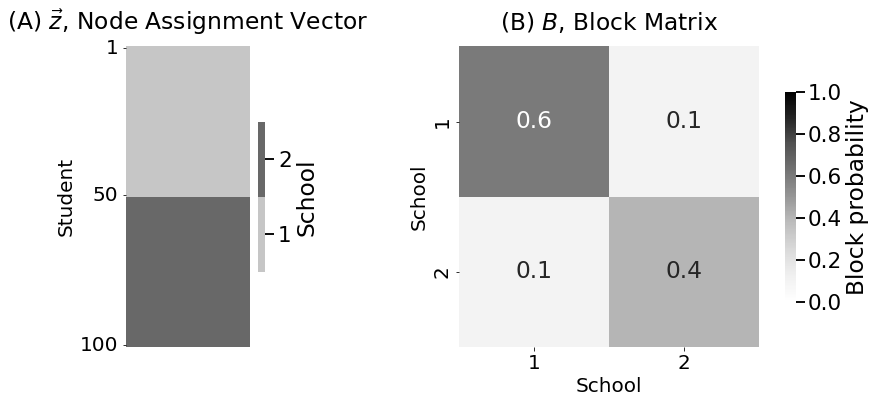
\includegraphics[width=\linewidth]{representations/ch5/Images/sbm.png}
    \caption[Parameters for a stochastic block model]{\textbf{(A)} the community assignment vector for each node (students). \textbf{(B)} the block matrix, which defines the probabilities of a pair nodes (students) from a given community having an edge.}
    \label{fig:ch5:sbm}
\end{figure}

Finally, let's sample and plot a single network from the $SBM_n(\vec z, B)$ with parameters $\vec z$ and $B$:

\begin{lstlisting}[style=python]
from graspologic.simulations import sbm
from graphbook_code import draw_multiplot

# sample a graph from SBM_{100}(tau, B)
A = sbm(n=[n//2, n//2], p=B, directed=False, loops=False)
ys = np.repeat([1, 2], 50)
draw_multiplot(A, labels=ys, title="$SBM_n(z, B)$ Simulation");
\end{lstlisting}

The adjacency matrix is shown in Figure \ref{fig:ch5:sbm_adj}(A).

The above network shows students, ordered by the school they are in (first school and the second school, respectively). As you can see in the network, people from the first school are more connected than people from school $2$. This heatmap can be described as \textit{modular}: it has clear community structure. The connections between people from different schools appear to be a bit {more sparse} (fewer edges) than connections between people from the same school.

When the nodes are ordered by community, we will often refer to ``patches'' (formally, \textit{subnetworks}, from Section \ref{sec:ch4:prop-net:subnetwork}) of the adjacency matrix as \textit{blocks}. The $(k, l)$ block of the adjacency matrix is the block of the adjacency matrix corresponding the the connections between nodes in community $k$ with nodes in community $l$. For instance, the $(1, 1)$ block of the adjacency matrix corresponds to the upper-left block, which is the subnetwork induced by the nodes from community $1$. The $(1,2)$ block of the adjacency matrix corresponds to the upper-right block, which is the subnetwork consisting of nodes in communities $1$ and $2$, but only the edges from nodes in community $1$ to nodes in community $2$. The blocks $(k, k)$ will be referred to as the \textit{on-diagonal} blocks, in that they are the blocks that occur along the diagonal of the adjacency matrix. The blocks $(k, l)$ where $k \neq l$ will be referred to as the \textit{off-diagonal} blocks, in that they are the blocks that do not fall right along the diagonal of the adjacency matrix. Here, the on-diagonal blocks look to have far more connections than the off-diagonal blocks.

In this case, the \textit{modular} structure simply suggests that the different blocks (distinguished by the communities of the different nodes) are readily apparent.


\subsection{Modularity is not a pre-requisite for $SBM_n(\vec z, B)$ random networks}
\label{sec:ch5:sbm:modularity}

Something easy to mistake about a sample of an SBM is that the samples will {not always} have the obvious modular structure you can see in Figure \ref{fig:ch5:sbm_adj}(A) when you look at a heatmap. Rather, this modular structure is {only} made obvious because the students are ordered according to the school in which they are in. What do you think will happen if you look at the students in a random order? Do you think that the structure that exists in this network will be obvious?

The answer is: {No!} Let's see what happens when we reorder the nodes from the network into a random order, and pretend you don't know the true community labels ahead of time:

\begin{lstlisting}[style=python]
import numpy as np

# generate a reordering of the n nodes
permutation = np.random.choice(n, size=n, replace=False)

Aperm = A[permutation][:,permutation]
yperm = ys[permutation]
heatmap(Aperm, title="Nodes randomly reordered")
\end{lstlisting}

\begin{figure}[h]
    \centering
    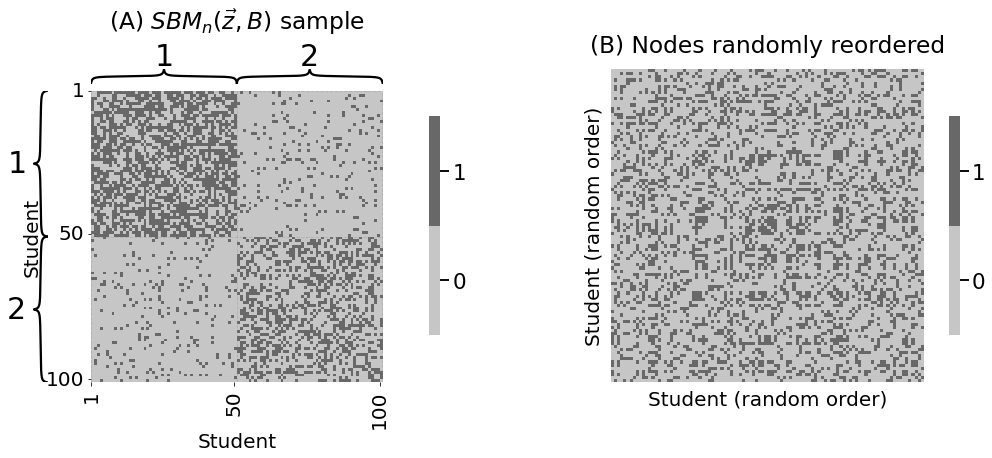
\includegraphics[width=\linewidth]{representations/ch5/Images/sbm_adj.png}
    \caption[Adjacency matrix for SBM with a community ordering of nodes and a random ordering of the nodes]{\textbf{(A)} the adjacency matrix for an $SBM_n(\vec z, B)$ simulation. The parameters are shown in Figure \ref{fig:ch5:sbm}. \textbf{(A)} the same adjacency matrix, but with the nodes randomly reordered.}
    \label{fig:ch5:sbm_adj}
\end{figure}
In Figure \ref{fig:ch5:sbm_adj}(B), the students are {not} organized according to school, because they have been randomly reordered. It becomes pretty tough to figure out whether there are communities just by looking at the adjacency matrix, unless you are looking at a network in which the nodes are {already arranged} in an order which respects the community structure. By an {order that respects the community structure}, we mean that the community assignment vector $\vec z$ is arranged so that all of the nodes in the first community come first, followed by all of the nodes in the second community, followed by all of the nodes in the third community, so on and so forth up to the nodes of the community $K$.

In practice, this means that if you know ahead of time what natural groupings of the nodes might be (such as knowing which school each student goes to) by way of your node attributes, you can visualize your data according to that grouping. This property is covered more in depth by \cite{Abbe2017Mar}. If you don't know anything about natural groupings of nodes, however, you are left with the problem of {estimating community structure}. A later method, called the {spectral embedding} in Section \ref{sec:ch6:spectral}, will be paired with clustering techniques to allow you to estimate node assignment vectors. 

We'll conclude off this section by showing that the previous random network model you saw, the ER random networks, are special cases of SBM random networks. These properties will become useful as you build more and more complex random network models, because when you develop techniques for more complex random network models in later chapters, they will extend directly to any network model which is a special case of that random network model.

\subsection{ER random networks are special cases of SBM random networks}

Let's imagine that you have a random network $\mathbf A$ which is $ER_n(p)$, an Erd\"os-R\'enyi network with probability $p$. Could you take this random network and turn it into an SBM? More specifically, does there exist an SBM such that the edge-existence probabilities are the same as the $ER_n(p)$ random network, for {every} edge in the network?

The answer is {always} a yes! This is extremely easy. Take the number of edge communities for the corresponding SBM to be $1$, and assign every node to the first community. Next, take the block matrix to have a single entry, $b_{11} = p$. And you are done! $\mathbf A$ is also an $SBM_n(\vec z, B)$ random network, where $\vec z$ is a vector of ones, and $B$ is a $1 \times 1$ matrix (really, just a scalar) whose only entry is $p$.

We are finished! To see that the edge-existence probabilities are the same, you'll back up to your coin flips. In the ER random network, you performed a coin flip for each edge $\mathbf a_{ij}$ with a coin that landed on heads with probability $p$. In the SBM random network, you performed a coin flip for each edge $\mathbf a_{ij}$ with a coin that landed on heads with probability $b_{z_i z_j}$. Here, there is only one possible value that $z_i$ or $z_j$ could take; they both must be one, since there is only one community. Therefore you flip a coin that lands on heads with probabaility $b_{11}$. But when you built the block matrix, we said that $b_{11}$ was just $p$, so the coin flip is occurring with a coin that lands on heads with probability $p$. This is obviously the same procedure you took with the ER random network at all possible edges, so the edge-existence probabilities are all identical. Therefore, the $ER_n(p)$ random network is also an $SBM_n([1, 1, ..., 1], B = [p])$ random network.

\subsection{Read on for more}

If you want a deeper level of technical depth on Stochastic Block Models, please see Appendix \ref{app:ch12:sbms}.


\newpage
\section{Random Dot Product Graphs}
\label{sec:ch5:rdpg}

Let's assume that you have $100$ people who live along a very long road that is $100$ miles long, and each person is $1$ mile apart. The nodes of your network represent the people who live along your assumed street, and the edges represent whether a given pair of people along the street are friends. However, there's a slight twist here: the people at the ends of the street are party hosts. If someone lives closer to one party host, they are going to tend to more frequently go to that host's parties than the other party host. Consequently, when someone lives near a party host, they are going to tend to be better friends with other people who go to that host's parties more frequently. How could you model such a situation?

Mathematically, for each person, we could have a vector $\vec x_i$, that looks like this:
\begin{align*}
    \vec x_i &= \begin{bmatrix}
        \frac{100 - i}{100} & \frac{i}{100}
    \end{bmatrix}
\end{align*}

We could model the probability of two people $i$ and $j$ being friends with $\vec x_i^\top \vec x_j$, the inner product. Remember that this quantity is just the element-wise sum of the elements of each vector; that is:
\begin{align*}
    \vec x_i^\top \vec x_j = \sum_{u = 1}^d x_{id}y_{jd}
\end{align*}

For instance, $\vec x_1 = \begin{bmatrix}1 \\ 0\end{bmatrix}$, and $\vec x_{100} = \begin{bmatrix} 0 \\ 1\end{bmatrix}$. Note that:
\begin{align*}
p_{1,100} = \vec x_1^\top \vec x_j = 1 \cdot 0 + 0 \cdot 1 = 0
\end{align*}
What happens in between?

Let's consider another person, person $30$. Note that person $30$ lives closer to person $1$ than to person $100$.  Here, $\vec x_{30} = \begin{bmatrix} \frac{7}{10}\\ \frac{3}{10}\end{bmatrix}$. This gives you that:
\begin{align*}
p_{1,30} &= \vec x_1^\top \vec x_{30} = \frac{7}{10}\cdot 1 + 0 \cdot \frac{3}{10} = \frac{7}{10} \\
p_{30, 100} &= \vec x_{30}^\top x_{100} = \frac{7}{10} \cdot 0 + \frac{3}{10} \cdot 1 = \frac{3}{10}
\end{align*}
So this means that person $1$ and person $30$ have a $70\%$ probability of being friends, but person $30$ and $100$ have only a $30\%$ probability of being friends.

This feels like it might work out for us, so let's formalize it a little bit. We will do this with the Random Dot Product Graph (RDPG). This concept was first introduced by \cite{Young2007}. With the RDPG, you can have random networks which are much more complex than those you saw with the $ER_n(p)$ and the $SBM_n(\vec z, B)$ random networks, but {still} have a discernable structure to them.

\subsection{Defining the RDPG}

\subsubsection{The latent position matrix}

We parameterize the RDPG using a matrix $X$ called the \textit{latent position matrix}. Each row $\vec x_i$ will be called the \textit{latent position of the node} $i$. In matrix form, $X$ looks like this:

\begin{align*}
 X = \begin{bmatrix}
     \vdash & \vec x_1^\top & \dashv \\
     \vdash & \vec x_2^\top & \dashv \\
     & \vdots & \\
     \vdash & \vec x_n^\top & \dashv
 \end{bmatrix}
\end{align*}

We will call the columns of $X$ the \textit{latent dimensions}, and the total number of columns that $X$ has will be called the \textit{latent dimensionality}. We will often use the letter $d$ to denote the latent dimensionality of the latent position matrix $X$. For this reason, we say that $X$ is an $n$ row (one for each node) and $d$ column (one for each latent dimension) matrix. Therefore, the latent position of the node $i$, $\vec x_i$, is a $d$-dimensional vector. 


\subsubsection{Conceptualizing the RDPG}

We call this model the RDPG because the probabilities of edges existing are based on {dot products} between pairs of latent positions for the different nodes in the network. The way that you can think of the RDPG random network is that the edges depend on a latent position matrix $X$. For each pair of nodes $i$ and $j$, you have a unique coin (we will call this the $(i,j)$ coin) which has a $\vec x_i^\top \vec x_j$ chance of landing on heads, and a $1 - \vec x_i^\top \vec x_j$ chance of landing on tails. If the $(i,j)$ coin lands on heads, the edge between nodes $i$ and $j$ exists, and if the $(i,j)$ coin lands on tails, the edge between nodes $i$ and $j$ does not exist. As before, this coin flip is performed independent of the coin flips for all of the other edges. If $\mathbf A$ is a random network which is $RDPG$ with a latent position matrix $X$, we say that $\mathbf A$ is an $RDPG_n(X)$ random network. 

\subsection{How do you simulate samples of $RDPG_n(X)$ random networks?}


The procedure in Algorithm \ref{alg:ch5:rdpg} will produce for you a network $A$, which has nodes and edges, where the underlying random network $\mathbf A$ is an RDPG random network. 

\begin{algorithm}[h]\caption{Simulating a sample from an $SBM_n(\vec z, B)$ random network}
\label{alg:ch5:rdpg}
\SetAlgoLined
\KwData{$n$ a number of nodes\newline $\vec X$ a latent position matrix whose rows indicate the $d$-dimensional latent position vectors for each node}
\KwResult{The adjacency matrix of a sample from the random network.}
\For{$i$ in $1$:$n$} {
    \For{$j > i$}{
        Obtain a weighted coin $(i,j)$ which has a probability of $\vec x_i^\top \vec x_j$ of landing on heads, and a $1 - \vec x_i^\top \vec x_j$ probability of landing on tails.

        Flip the $(i,j)$ coin, and if it lands on heads, the corresponding entry $a_{ij}$ in the adjacency matrix is $1$. If the coin lands on tails, the corresponding entry $a_{ij} = 0$.

        Let $a_{ji} = a_{ij}$.
    }
}

\end{algorithm}

Let's return to the party example we started above. The first thing that we need to worry about is deciphering what our latent position matrix looks like. Let's code it up below:

\begin{lstlisting}[style=python]
import numpy as np
from graphbook_code import lpm_heatmap

n = 100  # the number of nodes in your network
# design the latent position matrix X according to 
# the rules we laid out previously
X = np.zeros((n,2))
for i in range(0, n):
    X[i,:] = [(n - i)/n, i/n]

lpm_heatmap(X, ytitle="Person", xticks=[0.5, 1.5], xticklabels=[1, 2],
                xtitle="Latent Dimension", title="Latent Position Matrix, X")
\end{lstlisting}

This latent position matrix is shown in Figure \ref{fig:ch5:rdpg}(A). Next, we can use graspologic with this latent position matrix to sample an $RDPG_n(X)$ random network:

\begin{lstlisting}[style=python]
from graspologic.simulations import rdpg
from graphbook_code import heatmap

# sample an RDPG with the latent position matrix
# created above
A = rdpg(X, loops=False, directed=False)

# and plot it
heatmap(A.astype(int), xtitle="Person", ytitle="Person",
          title="$RDPG_{100}(X)$ Simulation")
\end{lstlisting}

A sample from the $RDPG_n(X)$ random network is shown in Figure \ref{fig:ch5:rdpg}(B).

\begin{figure}[h]
    \centering
    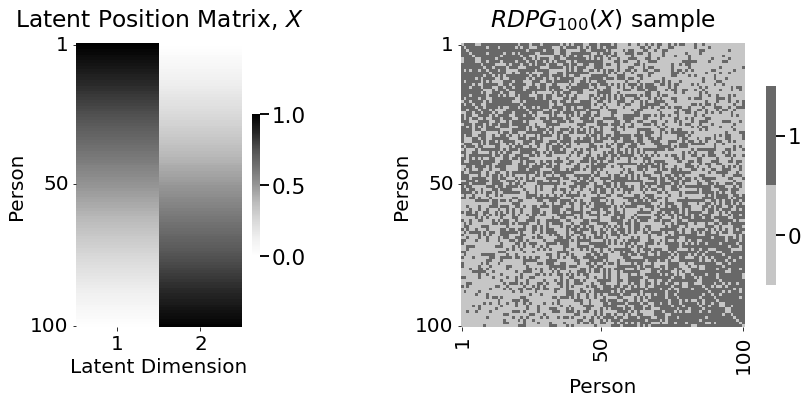
\includegraphics[width=\linewidth]{representations/ch5/Images/rdpg.png}
    \caption[Visualizing the Random Dot Product Graph]{\textbf{(A)} the latent position matrix. \textbf{(B)} a sample of an $RDPG_n(X)$ random network.}
    \label{fig:ch5:rdpg}
\end{figure}

\subsection{$RDPG_n(X)$ random networks generalizes to a broad class of problems}

In certain situations, the $RDPG_n(X)$ model can generalize the $SBM_n(\vec z, B)$ model that we learned about in Section \ref{sec:ch5:sbm}. The particular situation that the $RDPG_n(X)$ model is extremely effective for is known as {homophily} \cite{Hoff2007Dec,Athreya2017Jan}. Homophily exists in a network when the relationship between nodes which have similar characteristics (such as the same community assignment) are stronger than the relationships between nodes which have different characteristics (such as a pair of nodes with different community assignments). 

In the example that we covered in Section \ref{sec:ch5:sbm}, this is analogous to the idea that students from the same school were more likely to be friends than students from different schools. This is an extremely powerful concept, since many networks (and many network machine learning questions) that we will learn to ask will center around this concept of homophily.

To better understand when an $RDPG_n(X)$ random network will generalize an $SBM_n(\vec z, B)$ random network, we first will turn to the most generalizable independent-edge random network model: the Inhomogeneous Erd\"os R\'enyi Random Networks.

\subsection{Read on for more}

If you want a deeper level of technical depth on Random Dot Product Graphs, please see Appendix \ref{app:ch12:rdpg}.


\newpage
\section{Inhomogeneous Erd\"os-R\'enyi Random Networks}
\label{sec:ch5:ier}


Now that you've learned about the $ER_n(p)$, $SBM_n(\vec z, B)$, and $RDPG_n(X)$ random networks, it's time to figure out why we keep using coin flips! To this end, we will learn about the most general model for an independent edge random network, the Inhomogeneous Erdos Renyi (IER) Random Network.

\subsection{The Inhomogeneous Erdos-Renyi (IER) Random Network Model is parametrized by a matrix of independent-edge probabilities}

The IER random network is the most general random network model for a binary graph. The way you can think of the IER random network is that a probability matrix $P$ with $n$ rows and $n$ columns defines each of the edge-existence probabilities for pairs of nodes in the network. This is called the \textit{probability matrix} for the independent-edge random network model. For each pair of nodes $i$ and $j$, you have a unique coin which has a $p_{ij}$ chance of landing on heads, and a $1 - p_{ij}$ chance of landing on tails. If the coin lands on heads, the edge between nodes $i$ and $j$ exists, and if the coin lands on tails, the edge between nodes $i$ and $j$ does not exist. This coin flip is performed independently of the coin flips for all of the other edges. If $\mathbf A$ is a random network which is $IER$ with a probability matrix $P$, we say that $\mathbf A$ is an $IER_n(P)$ random network.

\subsubsection{Generating a sample from an $IER_n(P)$ random network}

As before, we develop a procedure in Algorithm \ref{alg:ch5:ier} to produce for you a network $A$, which has nodes and edges, where the underlying random network $\mathbf A$ is an $IER_n(P)$ random network.

\begin{algorithm}[h]\caption{Simulating a sample from an $IER_n(P)$ random network}
\label{alg:ch5:ier}
\SetAlgoLined
\KwData{$n$ a number of nodes \newline$P$ a probability matrix with $n$ rows and $n$ columns}
\KwResult{The adjacency matrix of a sample from the random network.}

\For{$i$ in $1$:$n$} {
    \For{$j > i$} {
        Obtain a weighted coin $(i,j)$ which has a probability $p_{ij}$ of landing on heads, and a $1 - p_{ij}$ probability of landing on tails.

        Flip the $(i,j)$ coin, and if it lands on heads, the corresponding entry $a_{ij}$ in the adjacency matrix is $1$. If the coin lands on tails, the corresponding entry $a_{ij}$ is $0$. 

        Set $a_{ji} = a_{ij}$.
    }
}
\Return{$A$}
\end{algorithm}

\begin{floatingbox}[h]\caption{$IER_n(P)$ and $SBM_n(\vec z, B)$ equivalence}
Notice that the model that we described for an $IER_n(P)$ random network is, in fact, equal to a very uninformative $SBM_n(\vec z, B)$ random network. If the network is simple, we could simply assign each node to its own community; e.g., the number of communities is $n$. Then, we can just let the block matrix $B$ be equal to the probability matrix $P$. However, if the number of communities is not equal to the number of nodes, this is not generally the case.
\end{floatingbox}

Let's create an example. We'll first generate a probability matrix that is unnecessarily complicated such that we couldn't capture it with the any Erd\"os R\'enyi, Stochastic Block Model with the fewer communities than nodes, nor an RDPG:

\begin{lstlisting}[style=python]
import numpy as np
from graphbook_code import heatmap

def generate_unit_circle(radius):
    diameter = 2*radius + 1
    rx = ry = diameter/2
    x, y = np.indices((diameter, diameter))

    circle_dist = np.hypot(rx - x, ry - y)
    diff_from_radius = np.abs(circle_dist - radius)
    less_than_half = diff_from_radius < 0.5

    return less_than_half.astype(int)

def add_smile():
    canvas = np.zeros((51, 51))
    canvas[2:45, 2:45] = generate_unit_circle(21)
    mask = np.zeros((51, 51), dtype=bool)
    mask[np.triu_indices_from(mask)] = True
    upper_left = np.rot90(mask)
    canvas[upper_left] = 0
    return canvas
    
def smile_probability(upper_p, lower_p):
    smiley = add_smile()
    P = generate_unit_circle(25)
    P[5:16, 25:36] = generate_unit_circle(5)
    P[smiley != 0] = smiley[smiley != 0]
    
    mask = np.zeros((51, 51), dtype=bool)
    mask[np.triu_indices_from(mask)] = True
    P[~mask] = 0
    P = (P + P.T - np.diag(np.diag(P))).astype(float)
    P[P == 1] = lower_p
    P[P == 0] = upper_p
    return P

P = smile_probability(.95, 0.05)
heatmap(P, vmin=0, vmax=1, title="Probability matrix $P$")
\end{lstlisting}

The probability matrix is plotted in Figure \ref{fig:ch5:ier}(A). Next, we can generate a random sample of the $IER_n(P)$ random network:

\begin{lstlisting}[style=python]
from graspologic.simulations import sample_edges

A = sample_edges(P, directed=False, loops=False)
heatmap(A.astype(int), title="$IER_n(P)$ sample")
\end{lstlisting}

The heatmap is shown in Figure \ref{fig:ch5:ier}(B). We used this example to show you that the key idea behind the IER Network's probability matrix is simple: the entries can really be anything as long as they are probabilities (between $0$ and $1$), and the resulting matrix is symmetric (in the case of undirected networks). There are no additional requirements nor parameters to add structure to the network.

\begin{figure}
    \centering
    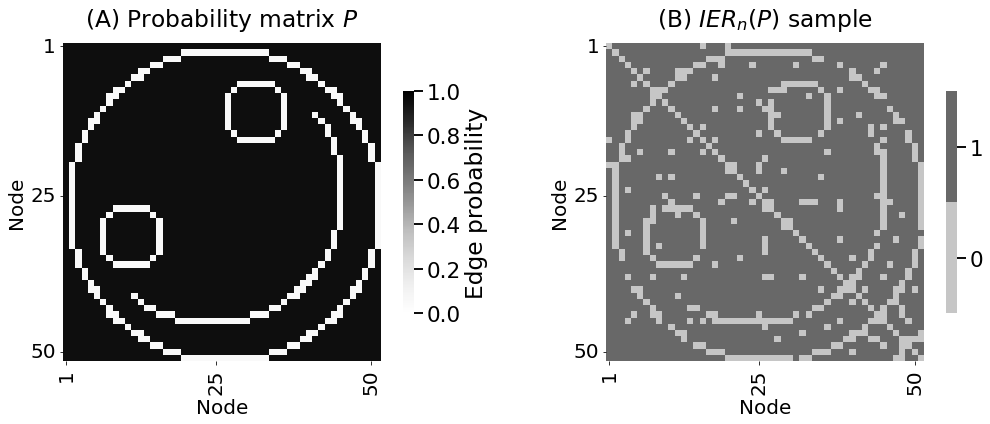
\includegraphics[width=\linewidth]{representations/ch5/Images/ier.png}
    \caption[$IER_n(P)$ parameters]{\textbf{(A)} the probability matrix for the $IER_n(P)$ random network. \textbf{(B)} an adjacency matrix sampled from the $IER_n(P)$ random network.}
    \label{fig:ch5:ier}
\end{figure}

\subsection{Unifying Independent-Edge Random Network Models}

The class of models that we have learned about so far are more generally known as independent-edge random networks \cite{Athreya2017Jan}. As it turns out, just like the $ER_n(p)$ random network was a special case of the $SBM_n(\vec z, B)$ random network, there are many other relationships that we can study as well. In this sense, we will study the ``hierarchy of network models''. A model is said to be more complex than a second model if we can generate the parameters of the first model using the parameters of the second model, but we cannot necessarily do the reverse.

\subsubsection{All independent-edge random networks are IER networks}
\label{sec:ch5:ier:ier_generalises}
The $IER_n(P)$ random network is more complex than every model that we have learned to date.
\begin{enumerate}
    \item Erd\"os R\'enyi with probability $p$: all entries $p_{ij}$ of $P$ can just be set equal to $p$
    \item Stochastic block model with community assignment vector $\vec z$ and block matrix $B$: construct the probability matrix $P$ such that $p_{ij} = b_{z_iz_j}$ of the block matrix $B$ where the communities of nodes $i$ and $j$ are $z_i$ and $z_j$, respectively.
    \item Random Dot Product Graph with latent position matrix $X$: Let there be a $P$ such that $P = XX^\top$. Note that the entries of $P$ by definition of matrix multiplication will be $p_{ij} = \vec x_i^\top \vec x_j$, which was exactly the relationship that we established in Section \ref{sec:ch5:rdpg}.
\end{enumerate}

\paragraph{How do we generate a probability matrix from a $SBM_n(\vec z, B)$?}
\label{sec:ch5:ier:sbm_pmtx}
One thing that will come up frequently over the course of this book is that we will need to sometimes programmatically generate the probability matrix directly (rather than just using the community assignment vector $\vec z$ and the block probability matrix $B$). This isn't too difficult to do, and some pseudocode is outlined in Algorithm \ref{alg:ch5:sbm_pmtx}.

\begin{algorithm}[h]\caption{Generating a probability matrix for a $SBM_n(\vec z, B)$ random network}
\label{alg:ch5:sbm_pmtx}
\SetAlgoLined
\KwData{$\vec z$ a community assignment vector for each of the $n$ nodes to one of $K$ communities\newline $B$ a block matrix with $K$ rows and $K$ columns}
\KwResult{The probability matrix associated with the $SBM_n(\vec z, B)$.}

Construct a matrix $C$ with $n$ rows and $K$ columns; one row for each node, and one column for each community.

\For{$i$ in $1$:$n$} {
    \For{$k$ in $1$:$K$} {
        If $z_i = k$, let $c_{ik} = 1$. If $z_i \neq k$, let $c_{ik} = 0$.
    }
}

Let $P = CBC^\top$.
\end{algorithm}

Let's break down exactly how this works. The matrix $C$ is better known as a one-hot encoding of the vector $\vec z$. When we multiply $CB$, the matrix product will be the $n \times k$ matrix:
\begin{align*}
    (CB)_{ik} = \sum_{l = 1}^Kc_{il} b_{lk}.
\end{align*}
However, we know that $c_{il} = 1$ if $z_i = l$, and $0$ otherwise. So for each entry:
\begin{align*}
    (CB)_{ik} = b_{z_i k}
\end{align*}
This matrix is going to end up looking something like this:
\begin{align*}
    CB = \begin{bmatrix}
        b_{z_i1} & \hdots & 
        b_{z_iK} \\
        \vdots & \ddots & \vdots \\
        b_{z_n1} & \hdots & b_{z_n K}
    \end{bmatrix}.
\end{align*}
So each row of $CB$ corresponds to a single node $i$ in the network, identifies the community of that node, and then ``extracts'' from the block matrix all of the other communities that another node $j$ could possibly be in. This means that the $i^{th}$ row of the matrix $CB$ delineates all possible probabilities that a node in the network could have with other nodes in the network (depending on the other node's community, which is indicated in the column).

Multiplying the $CB$ matrix by $C^\top$ allows us to relate the probability information to the other nodes in the network. This step takes the probabilities for a given node $i$ with other nodes of arbitrary community (from the $CB$ matrix), and then cross-references them with the actual communities that nodes in the network are a part of.

When we right-multiply by $C^\top$, what we get is:
\begin{align*}
    (CBC^\top)_{ij} = \sum_{l = 1}^Kc_{jl}b_{z_il}.
\end{align*}
As before, $c_{jl} = 1$ if $z_j = l$, and $0$ otherwise. So for each entry:
\begin{align*}
    p_{ij} = (CBC^\top)_{ij} = b_{z_i z_j}. \numberthis \label{eqn:ch5:ier:sbm_p}
\end{align*}

So, $C$ encodes the community of each source node, $B$ provides the connection probabilities between communities, and $C^\top$ encodes the community of each target node. The result, $p_{ij} = (CBC^\top)_{ij}$, gives the probability that node $i$ and node $j$ are connected in the network, given their community assignments. Notice that this aligns exactly with the result that we obtained in Section \ref{sec:ch5:ier:ier_generalises}.  


Let's work through this example programmatically, because it comes up a few times over the course of the book. Let's imagine that we have $50$ nodes, of which the first $25$ are in community one and the second $25$ are in community two. The code to do this conversion looks like this:

\begin{lstlisting}[style=python]
def encode(community_assignments):
    """
    A function to generate the one-hot-encoded community
    assignment matrix from a community assignment vector.
    """
    z = community_assignments
    K = len(np.unique(z))
    n = len(z)
    C = np.zeros((n, K))
    for i, zi in enumerate(z):
        C[i, zi - 1] = 1
    return C

def sbm_probabilities(z, B):
    """
    A function to generate the probability matrix for an SBM.
    """
    C = encode(z)
    return C @ B @ C.T

# the community assignment vector
z = np.repeat([1, 2], 25)
# block matrix
B = np.array([[0.6, 0.3], 
              [0.3, 0.6]])
# probability matrix
P = sbm_probabilities(z, B)
\end{lstlisting}

The relationship between the community assignment vector, the community assignment matrix, the block matrix, and the probability matrix is illustrated in Figure \ref{fig:ch5:ier:sbm}.

\begin{figure}
    \centering
    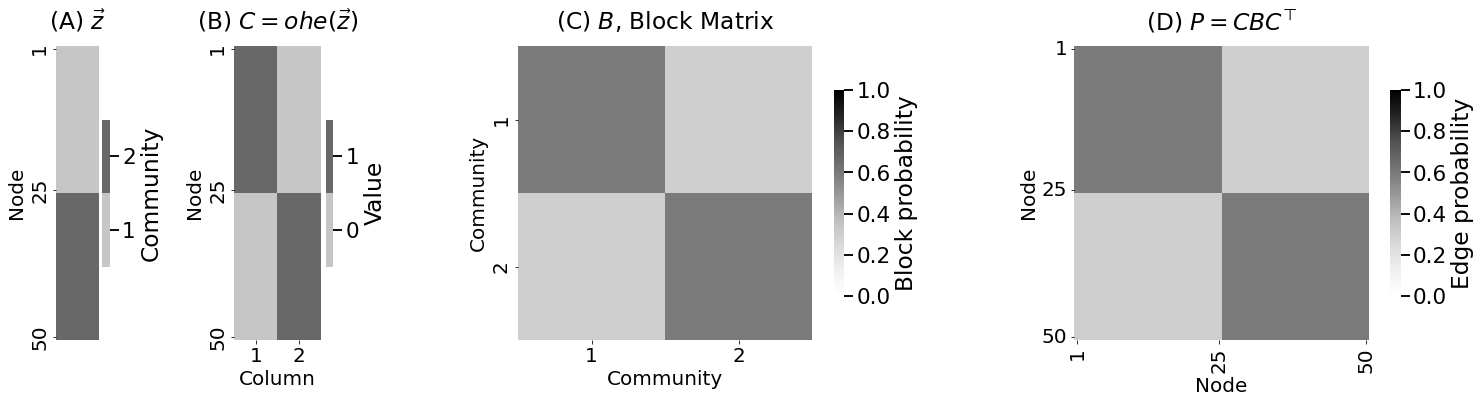
\includegraphics[width=\linewidth]{representations/ch5/Images/sbm_prob.png}
    \caption[Deriving probability matrix for $SBM_n(\vec z, B)$ random network.]{\textbf{(A)} the community assignment vector $\vec z$ and \textbf{(B)} the community assignment matrix $C$. Notice that each node has a value of $1$ in the corresponding column in which the node is a community. The first 25 nodes have a value of $1$ in column $1$, and the second $25$ nodes have a value of $1$ in column $2$. \textbf{(C)} the block matrix. \textbf{(D)} the probability matrix for each node pair.}
    \label{fig:ch5:ier:sbm}
\end{figure}

\subsubsection{What is the difference in complexity between the $SBM_n(\vec z, B)$ and $RDPG_n(X)$?}
\label{sec:ch5:ier:rdpg_sbm}

$RDPG_n(X)$ is a trivially more complex class of random networks than $ER_n(p)$. Choose $X$ to be a matrix with $n$ rows and $1$ column, where every entry is $\sqrt p$). However, the complexity relationship between the $SBM_n(\vec z, B)$ random networks and a $RDPG_n(X)$ is not as obvious. 

When the number of communities is less than the number of nodes, the street example that we gave in Section \ref{sec:ch5:rdpg} is sufficient to prove that $RDPG_n(X)$ is not a special case of $SBM_n(\vec z, B)$ with $K < n$; that is, there are $RDPG_n(X)$ random networks that are not $SBM_n(\vec z, B)$ random networks. The street example cannot be captured with an SBM unless we take the number of communities equal to the number of nodes. You will better understand why this is the case in Section \ref{sec:ch5:psd_block:same_lp}.

Notice, on the other hand, that if we are given a probability matrix $P$, and if there exists a matrix $X$ where $P = XX^\top$, that we could build an $RDPG_n(X)$ random network by using the matrix $X$ as the latent position matrix. This condition is equivalent to stating that $P$ must be positive semi-definite \cite{Athreya2017Jan,Rubin2022Sep}.

In the case of an $SBM_n(\vec z, B)$ random network, the probability matrix $P = CBC^\top$ will be positive semi-definite whenever $B$ is positive semi-definite \cite{Chung2021Mar,Athreya2017Jan}. This would mean that $B$ can be written as the product of a matrix $\sqrt B$ and its transpose $\sqrt B^\top$. In this case, if we took the latent position matrix $X$ to be $C\sqrt B$, we would get that:
\begin{align*}
    XX^\top &= C\sqrt B\sqrt B^\top C^\top \numberthis\label{eq:ch5:ier:sbm_rdpg}\\
    &= CBC^\top,
\end{align*}
which is the probability matrix of a $SBM_n(\vec z, B)$ random network. This shows that every SBM with a positive semi-definite block matrix can be transformed into an RDPG. Thus the $RDPG_n(X)$ is more complex than the $SBM_n(\vec z, B)$ with a positive semi-definite block matrix and a number of communities less than the number of nodes. 

Going into too much more depth about the concept of positive semi-definiteness would get outside this book's scope, so we will leave you with some practical guidance on several types of positive semi-definite block matrices in Section \ref{sec:ch5:psd_block}. If you want more technical depth, we would recommend a matrix analysis book like \cite{Horn2012Oct}. 

To check if a given block matrix \texttt{B} is positive semi-definite, you can use this utility, which builds upon concepts from \cite{Horn2012Oct}:

\begin{lstlisting}[style=python]
def is_psd(B):
    """
    A function which indicates whether a block matrix
    B is positive semi-definite.
    """
    return np.all(np.linalg.eigvals(B) >= 0)
is_psd(B)
# True
\end{lstlisting}

Consequently, this will tell you whether your $SBM_n(\vec z, B)$ random network can be described by an $RDPG_n(X)$ random network.

\paragraph{A more general RDPG}
\label{sec:ch5:ier:grdpg}
The aptly-named Generalized Random Dot Product Graph \cite{Rubin2022Sep}, or gRDPG, allows you to capture block matrices which are not positive semi-definite, also known as indefinite. This model underlies the theoretical motivation for many techniques that we will describe in Chapter \ref{sec:ch6}. The technical and theoretical details of these types of RDPGs are beyond the scope of this book, although some statistical formalization is provided in Appendix \ref{app:ch12:rdpg}.

\subsubsection{The hierarchy of independent-edge random network models}

In general, the ``hierarchy of complexity'' of our network models is shown in Figure \ref{fig:ch5:hierarchy}. The circles indicate the breadth of problems that the particular network model can be used to describe. If one model is entirely contained within another, that every random network described by the contained model can also be described by the subsuming model (where the reverse is not true). If the two models overlap, it means that some random networks described by one of the models can also be described by the other model, but not necessarily always.

To succinctly summarize what we've learned so far:
\begin{enumerate}
    \item $ER_n(p)$ random networks are less complex than $SBM_n(\vec z, B)$ with $K < n$: choose a $1$-community $SBM$ with a block matrix of $B = [p]$.
    \item $ER_n(p)$ random networks are less complex than $RDPG_n(X)$: could choose the latent position matrix to be a $1$-column matrix whose only entry is $\sqrt p$.
    \item $SBM_n(\vec z, B)$ with $K < n$ and positive semi-definite $B$ is less complex than $RDPG_n(X)$: Let $\sqrt B$ be the square-root of the matrix $B$, and $C$ the one-hot encoding of the matrix $\vec z$. Take $X = C\sqrt B$.
    \item $SBM_n(\vec z, B)$ with $K < n$ and indefinite $B$ is not describable with $RDPG_n(X)$: indefinite $B$ produces an indefinite $P$ matrix, and $RDPG_n(X)$ can only describe positive semi-definite $P$ matrices.
    \item Some $RDPG_n(X)$ are not describable by a $SBM_n(\vec z, B)$ with $K < n$: take the street example, from Section \ref{sec:ch5:rdpg}. This cannot be described by a $SBM_n(\vec z, B)$ with $K < n$.
    \item All $ER_n(p)$ random networks, $SBM_n(\vec z, B)$ random networks with $K < n$, and $RDPG_n(X)$ are less complex than $IER_n(P)$: all independent-edge random networks are sub-types of $IER_n(P)$. So it must be the most complex.
    \item $IER_n(P)$ random networks are equivalent in complexity to $SBM_n(\vec z, B)$ random networks with $K = n$: With $K = n$, the block matrix $B$ is $n \times n$, and can be chosen to be equal to the probability matrix $P$.
\end{enumerate}

\begin{figure}
    \centering
    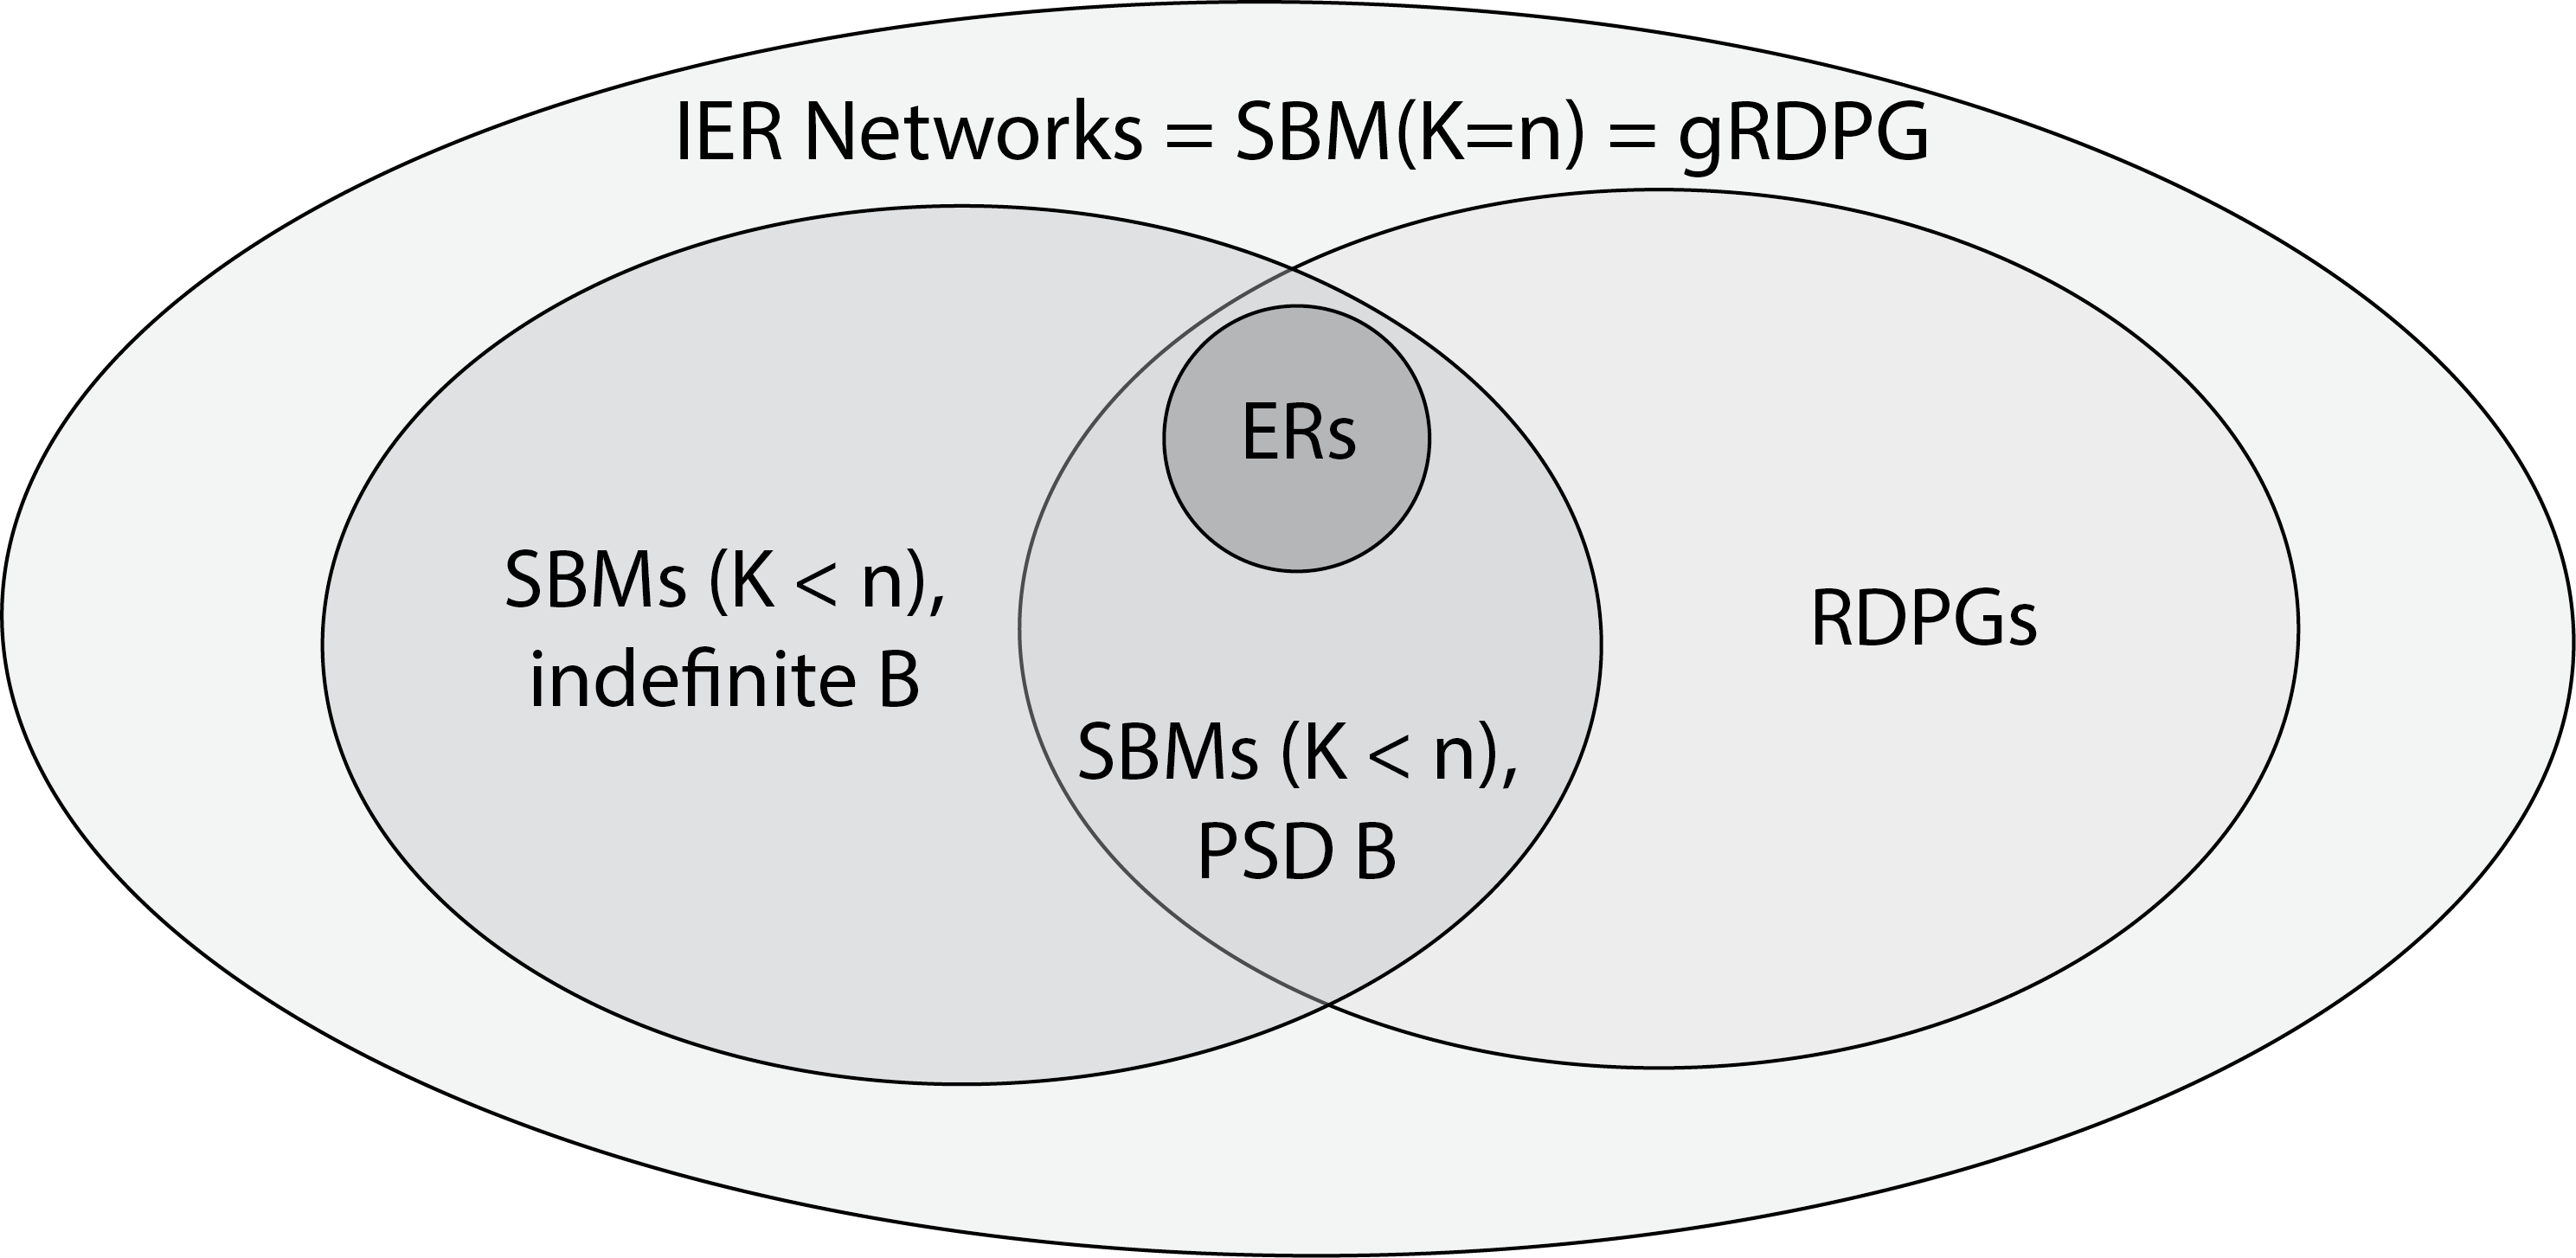
\includegraphics[width=\linewidth]{representations/ch5/Images/unify_sn.png}
    \caption{The hierarchy of complexity for Random Network Models.}
    \label{fig:ch5:hierarchy}
\end{figure}

\subsection{Read on for more}

If you want a deeper level of technical depth on Inhomogeneous Erd\"os R\'enyi Random Networks, please see Appendix \ref{app:ch12:rdpg}.


\newpage
\section{Properties of random networks}
\label{sec:ch5:prop}

In this section, we'll take a step back and appreciate some of the other descriptive properties that we can use to describe random networks. We will review many ideas that we discussed in Chapter \ref{sec:ch4}, which were properties and statistics that we can calculate for networks. These ideas will be reformulated for random networks that you have learned about in this Chapter. 

The key distinction is that unlike networks you've already observed (which have nodes and edges), random networks have nodes and potential edges which exist (or do not) with some probability. This means that properties of these networks will not be exact values; rather, they will be random quantities. However, we can still describe these random quantities using basic concepts from statistics. 

\subsection{A quick recap of expected values}

The principal result that we will use for this section is the expected value of binary quantities. If $\mathbf x$ is a random quantity that has the value $1$ with probability $p$ and $0$ with probability $1 - p$, $\mathbf x$ is what is known as Bernoulli distributed with probability $p$. This is basically the equivalent of a coin flip experiment, where a value of heads is recorded as a $1$, and a value of tails is recorded as a $0$. The coin may or may not be fair, in that the probability that it lands on heads might differ from $0.5$. 

In these contexts, the outcome is not yet realized for the random quantity (it is random after all). Instead, we describe properties about the random quantity, which tell us information about how we expect this random quantity to behave. The one that we will be most interested in is known as the expected value, which is denoted as $\mathbb E[\cdot]$. The expected value of a binary ($0$ or $1$)-valued quantity $\mathbf x$ is:
\begin{align*}
    \mathbb E[\mathbf x] &= 0 Pr(\mathbf x = 0) + 1 Pr(\mathbf x = 1) \\
    &= Pr(\mathbf x = 1).\numberthis\label{eqn:ch5:exp:binary}
\end{align*}
This can be informally thought of as the average value that the random quantity takes over infinitely many trials. 

So, if a coin lands on heads (a value of $1$) with probability $0.75$, its expected value is $0.75$. 

Another key result that we will need to know about expected values is that they behave linearly under finite sums. This simply means that if $\mathbf x$ and $\mathbf y$ are two finite quantities, that:
\begin{align*}
    \mathbb E[\mathbf x + \mathbf y] = \mathbb E[\mathbf x] + \mathbb E[\mathbf y].\numberthis\label{eqn:ch5:exp:linearity}
\end{align*}
So, if $\mathbf x$ is a coin flip that lands on heads with probability $0.75$ and $\mathbf y$ is a flip of a different coin that lands on heads with probability $0.25$, the expected value of their sum is $1.0$. Easy enough, right?

Next up is the rescaling property of expected values. If $\alpha$ is a constant (a non-random quantity), then:
\begin{align*}
    \mathbb E[\alpha \mathbf x] &= \alpha \mathbb E[\mathbf x].\numberthis\label{eqn:ch5:exp:rescale}
\end{align*}
So, for instance, let's imagine that $\mathbf x$ is a coin flip that lands on heads with probability $0.75$. Let's say that we decide to play a game where, if the coin lands on heads, we give you $\$5$, but if it lands on tails you get $\$0$. Using this rule, notice that we could just multiply the value of the coin flip outcome by $5$ (if the coin lands on a $1$, or heads, the outcome is $5$, and if it lands on a $0$, or tails, the outcome is $5 \cdot 0 = 0$). Then the expected outcome is:
\begin{align*}
    \mathbb E[5 \mathbf x] &= 5 \mathbb E[\mathbf x] \\
    &= 5 \cdot .75 = \frac{15}{4},
\end{align*}
and you are expected to make $\$\frac{15}{4}$ from this game.

\subsection{Rethinking edge probabilities as expected values}

The equation that you saw in Equation \eqref{eqn:ch5:exp:binary} should look very familiar to you. Remember that in a network, $\mathbf a_{ij}$ is just a binary quantity, like $\mathbf x$.

Remember that if $\mathbf A$ is a $IER_n(P)$ random network, the probability matrix $P$ has entries $p_{ij}$ for each pair of nodes $i$ and $j$ that describe the probability that $\mathbf a_{ij}$ has a value of $1$.

This means that we can compute the expected value of each adjacency in the network using the formula, as:
\begin{align*}
    \mathbb E[\mathbf a_{ij}] = p_{ij}.\numberthis\label{eqn:ch5:exp:prob}
\end{align*}

Crucially, this gives us the insight that the probability matrix can also be thought of as the expected value of the adjacency matrix for a random network:
\begin{align*}
    \mathbb E[\mathbf A] &= \begin{bmatrix}
        \mathbb E[\mathbf a_{11}] & \hdots & \mathbb E[\mathbf a_{1n}] \\
        \vdots & \ddots & \vdots \\
        \mathbb E[\mathbf a_{n1}] & \hdots & \mathbb E[\mathbf a_{nn}]
    \end{bmatrix} = P.
\end{align*}

\subsection{Random node degree}
\label{sec:ch5:prop:rndeg}

Remember that the degree of a node $i$ was defined as:
\begin{align*}
    d_i &= degree(i) = \sum_{j \neq i} a_{ij}.
\end{align*}
Similarly, the \textit{random node degree} for a random network $\mathbf A$ is defined as:
\begin{align*}
    \mathbf d_i &= \sum_{j \neq i}\mathbf a_{ij}.
\end{align*}
This quantity is random, in that it is not necessarily any particular value: it takes a number of possible values with a probability. We can use the properties that we learned above to compute the expected degree:
\begin{align*}
    \mathbb E[\mathbf d_i] &= \mathbb E\left[\sum_{j \neq i}\mathbf a_{ij}\right] \\
    &= \sum_{j \neq i}\mathbb E[\mathbf a_{ij}],\numberthis \label{eqn:ch5:exp:deg:e1}
\end{align*}
Which is a direct consequence of Equation \eqref{eqn:ch5:exp:linearity}. Let's imagine that there are $n > 3$ nodes in the network, and $i = 1$. This means that:
\begin{align*}
    \mathbb E[\mathbf d_1] &= \mathbb E\left[\sum_{j \neq 1} \mathbf a_{1j} \right] = \mathbb E\left[\sum_{j \geq 2} \mathbf a_{1j} \right]\\
    &= \mathbb E[\mathbf a_{12}] + \mathbb E\left[\sum_{j \geq 3} \mathbf a_{1j} \right],
\end{align*}
which is a direct application of the result of Equation \eqref{eqn:ch5:exp:linearity}. Next, we can write down $\mathbb E\left[\sum_{j \geq 3} \mathbf a_{1j} \right]$ as a sum of $\mathbb E[\mathbf a_{13}]$ and $\mathbb E\left[\sum_{j \geq 4} \mathbf a_{1j} \right]$, and we can continue this pattern all the way up to $n$ to get the result in Equation \eqref{eqn:ch5:exp:deg:e1}. 

Continuing from Equation \eqref{eqn:ch5:exp:deg:e1}, remember that $\mathbb E[\mathbf a_{ij}] = p_{ij}$ by Equation \eqref{eqn:ch5:exp:prob}. So, the \textit{expected node degree} is:
\begin{align*}
    \mathbb E[\mathbf d_i] &= \sum_{j \neq i}p_{ij}.\numberthis\label{eqn:ch5:exp:expdeg}
\end{align*}
\begin{floatingbox}[h]\caption{Expected degree in an $SBM_n(\vec z, B)$ random network is constant within a community}
Imagine that you have a network $\mathbf A$ that is an $SBM_n(\vec z, B)$ random network. Suppose that for $n$ nodes, $n/2$ of the nodes are in community $1$, and $n/2$ of the nodes are in community $2$. Consider the block matrix:
\begin{align*}
    B &= \begin{bmatrix}
        0.5 & 0.2 \\
        0.2 & 0.3
    \end{bmatrix}.
\end{align*}
\begin{enumerate}
    \item With $n=100$, compute the degree of each node in the network. 
    \item Repeat the above simulation $R=100$ times, keeping track of your results in a data frame with the columns as the node index $i$, the community that the node $i$ is in, the simulation replicate $r$, and the node degree $d_{i}^{(r)}$. 
    \item Compute the average degree for each node across all simulations. This should reduce your data frame to node index $i$, community that the node $i$ is in, and the average node degree over all simulations.
    \item Explain what you observe about the average degrees for each node in a particular community (the nodes of the same community have$\hdots$ average node degrees, and nodes in different communities have $\hdots$ average node degrees). 
    \item Establish an equation for the expected node degree for a node $i$, for each of the two communities. Explain how this supports your answer that you obtained in 4.
\end{enumerate}
\end{floatingbox}

\subsubsection{Random network density}
\label{sec:ch5:prop:rndens}
Likewise, the \textit{density of a random network} $\mathbf A$ is defined as:
\begin{align*}
    density(\mathbf A) &= \frac{\sum_{j > i}\mathbf a_{ij}}{\binom n 2}
\end{align*}
As before, this quantity is random, so it does not have any particular value. However, its expected value can be computed using the rules that we described above exactly.

First, notice that if the network has $n$ nodes, $\binom n 2$ is simply a constant. This means that:
\begin{align*}
    \mathbb E[density(\mathbf A)] &= \mathbb E\left[\frac{\sum_{j > i}\mathbf a_{ij}}{\binom n 2}\right] \\
    &= \frac{1}{\binom n 2}\mathbb E\left[\sum_{j > i}\mathbf a_{ij}\right],
\end{align*}
which is from Equation \eqref{eqn:ch5:exp:rescale}. Next, we can use the linearity argument from Equation \eqref{eqn:ch5:exp:linearity} to obtain:
\begin{align*}
    \mathbb E[density(\mathbf A)] &= \frac{1}{\binom n 2}\sum_{j > i}\mathbb E[\mathbf a_{ij}] \\
    &= \frac{1}{\binom n 2}\sum_{j > i}p_{ij}.\numberthis\label{eqn:ch5:exp:expdens}
\end{align*}
Using Equations \eqref{eqn:ch5:exp:expdeg} and \eqref{eqn:ch5:exp:expdens}, we can draw the same conclusions that we did in Section \ref{sec:ch4:prop-net:degree} to conclude that:
\begin{align*}
    \mathbb E[density(\mathbf A)] &= \frac{\sum_{i = 1}^n \mathbb E[\mathbf d_i]}{n(n - 1)}.\numberthis \label{eqn:ch5:exp:expdens:e0}
\end{align*}
Finally, remember that $d = \frac{1}{n}\sum_{i = 1}^n d_i$ is the average degree of the nodes in a network $A$. 

Likewise, $\mathbf d = \frac{1}{n}\sum_{i = 1}^n \mathbf d_i$ is the average degree of nodes in a random network $\mathbf A$. Again, since this quantity is random, it can be summarized using expected values. Since $n$ is a fixed number of nodes, then:

\begin{align*}
    \mathbb E\left[\mathbf d\right] &= \mathbb E\left[\frac{1}{n}\sum_{i = 1}^n \mathbf d_i\right] \\
    &= \frac{1}{n}\mathbb E\left[\sum_{i = 1}^n \mathbf d_i\right],
\end{align*}
using the rescaling property in Equation \eqref{eqn:ch5:exp:rescale}. Finally, using the linearity of sums in Equation \eqref{eqn:ch5:exp:linearity}:
\begin{align*}
    \mathbb E\left[\mathbf d\right] &= \frac{1}{n}\sum_{i = 1}^n \mathbb E[\mathbf d_i].
\end{align*}
Combining this with Equation \eqref{eqn:ch5:exp:expdens:e0}:
\begin{align*}
    \mathbb E[density(\mathbf A)] &= \frac{\mathbb E[\mathbf d]}{n - 1}.
\end{align*}
Just like the density of a network $A$ could be conceptualized as the average degree of each node in the network, the expected density of a random network $\mathbf A$ can be conceptualized as the average expected degree of each node in the random network.

\subsection{Population network laplacian}
\label{sec:ch5:prop:poplapl}
Remember in Section \ref{sec:ch4:mtx-rep:dad_laplacian}, you learned that the \texttt{DAD} Laplacian was defined as a function of a adjacency matrix:
\begin{align*}
    L &= D^{-\frac{1}{2}}AD^{-\frac{1}{2}}\numberthis \label{eqn:ch5:dad}
\end{align*}
This was a function of the adjacency matrix because it is a product of the adjacency matrix pre and post-multiplied by a function of the adjacency matrix (the inverse square-root of the degree matrix, $D$). 

Basically, the idea is that the population network Laplacian $\mathcal L$ is to the random network $\mathbf A$ what the \texttt{DAD} Laplacian $L$ was to the adjacency matrix $A$.

The population network Laplacian is:
\begin{align*}
    \mathcal L &= \mathcal D^{-\frac{1}{2}} P \mathcal D^{-\frac{1}{2}}. \numberthis \label{eqn:ch6:lse:poplapl}
\end{align*}

The matrices $\mathcal D$ (note the cursive script instead of the $D$ script, to contrast it from the degree matrix of a network sample) here are what is known as the \textit{expected degree matrix}. 

In the case of simple $IER_n(P)$ random networks, this is the diagonal matrix whose diagonal entries are:
\begin{align*}
    \mathbb E[\mathbf d_i] &= \sum_{j \neq i} p_{ij}.\numberthis \label{eqn:ch6:lse:e1}
\end{align*}

The only thing that you need to know for the purposes of this book is some intuition about this quantity. The expected degree matrix looks like this:

\begin{align*}
    \mathcal D &= \begin{bmatrix}
        \mathbb E[d_1] & & \\
        & \ddots & \\
        & & \mathbb E[d_n]
    \end{bmatrix} = \begin{bmatrix}
\sum_{j \neq 1} p_{1j} & & \\
& \ddots & \\
& & \sum_{j \neq n} p_{nj}
    \end{bmatrix}.
\end{align*}

So, it is a diagonal matrix, and is a function of the probability matrix $P$ (just like the degree matrix was a function of the adjacency matrix, for network samples). 

The diagonal entries of $\mathcal D$, $\mathbb E[d_i]$, give the expected number of edges that you would expect a node $i$ to  have in a given network sample.

A natural choice for the inverted square-root matrix of $\mathcal D$ would be:

\begin{align*}
    \mathcal D^{-\frac{1}{2}} &= \begin{bmatrix}
        \frac{1}{\sqrt{\mathbb E[d_1]}} & & \\
        & \ddots & \\
        & & \frac{1}{\sqrt{\mathbb E[d_1]}}
    \end{bmatrix} 
\end{align*}

Notice that as long as every node does not have a probability of zero of being connected to any other nodes in the network, this quantity exists and is finite. This is because if any node $i$ had a probability of zero of being connected to all of the other nodes of the network, then $\sum_{j \neq i} p_{ij} = \sum_{j \neq i} 0 = 0$, and hence, $\frac{1}{0} = \infty$. We will describe this restriction using the language that, for every node $i$, at least one other node $j$ exists where $p_{ij} > 0$.

With the restriction in mind, all of the entries along the diagonal of $\mathcal D$ are going to be positive values. This means that their reciprocals $\frac{1}{\mathbb E[d_i]}$ and the square roots of their reciprocals $\frac{1}{\sqrt{\mathbb E[d_i]}}$ will also be positive values.

In this sense, $\mathcal L$ can be thought of as the expected \texttt{DAD} Laplacian for a random network $\mathbf A$. It is the same equation as $L$ in Equation \eqref{eqn:ch5:dad}, except instead of thinking about the adjacency matrix/degree of a given matrix $A$, we are thinking about the expected adjacency matrix (the probability matrix, $P$) and the expected degree matrix $\mathcal D$ for the random network $\mathbf A$. 

\newpage
\section{Degree-Corrected Stochastic Block Models}
\label{sec:ch5:dcsbm}


For this network model, we're going to start off with the school example that we covered in Section \ref{sec:ch5:sbm}. Remember that there are $100$ students, who each attend one of two schools. The edges of the network represent whether a pair of students are friends. If two students attend the same school, they have a higher chance of being friends than if they attend different schools. 

In a lot of real-world networks, this model works pretty effectively. It captures ``community structure'' in a very succinct way, but it has a glaring weakness. To explore this weakness, we would recommend that more advanced statistics users check out the Appendix Section \ref{sec:app:ch12:dcsbms}. Basically, the idea is this: within a given community, we have {no way} to represent fundamental differences between nodes in our SBM. Stated another way, if node $i$ and node $j$ are both in the same commuity, they will, on average, have the same {node degree}, which is a concept that you learned about in Section \ref{sec:ch4:prop-net:degree}. 

Rotating back to our school example from Section \ref{sec:ch5:sbm} to put this into context, on average, students in the network will have the same number of friends. This is referred to as the \textit{degree homogeneity} (the expected degrees are the same) for all nodes in the same community. Fortunately, there is a relatively easy way that we can rectify this issue and obtain a network model which does not suffer from this limitation: the degree-correction vector.

\subsection{The degree-correction vector allows us to convey node "importance"}

The reason that this equality in the number of expected ``friends'' for each student is problematic is that in real world networks, some nodes are more ``popular'' than others. This can be more generically conceptualized as some nodes being more ``important'' than others, in that they have a higher number of edges on average than other nodes in the network. This is known as \textit{degree heterogeneity}. The first two parameters of the DCSBM are the same as the SBM, in that we have a community assignment vector, and a block matrix.

The way that the degree heterogeneity is conveyed in a DCSBM is via the \textit{degree-correction vector} $\vec\theta$, which has $n$ elements (one for each node). For each node $i$, the degree-correction factor $\theta_i$ simply ``degree-corrects'' the node $i$, by either ``amplifying'' its expected node degree (meaning, on average, node $i$ will have {more} edges than it would if it were a node in a $SBM_n(\vec z, B)$) when $\theta_i > 1$, or ``reducing'' its expected node degree (meaning, on average, node $i$ will have {fewer} edges than it would if it were a node in a $SBM_n(\vec z, B)$) when $\theta_i < 1$. In general, degree correction factors are always taken to be $\geq 0$, which means that we cannot have a negative degree-correction factor. 

Rotating back to our coin flip example from Section \ref{sec:ch5:sbm}, let's conceptualize how we can break this down. For a given node pair of nodes $i$ and $j$, we look first at the community assignments of each of these nodes $z_{i}$ and $z_j$. Then, we take the corresponding entry from the block matrix, $b_{z_i z_j}$, which corresponds to the ``base'' probability that node $i$ and node $j$ are connected. Finally, we inflate (or deflate) this probability based on the degree-correction factors. We obtain a coin which lands on heads with probability $\theta_i \theta_j b_{z_iz_j}$, where $\theta_i$ and $\theta_j$ are the degree-correction factors for nodes $i$ and $j$. This gives us the probability of an edge $(i, j)$ existing between any given pair of nodes $i$ and $j$.

If $\mathbf A$ is a DCSBM random network with $n$ nodes, the community vector $\vec z$, the block matrix $B$, and the degree-correction factor $\vec\theta$, we say that $\mathbf A$ is a $DCSBM_n(\vec z, \vec \theta, B)$ random network. 

\subsection{Unifying $DCSBM_n(\vec z, \vec\theta, B)$ networks with the hierarchy of random network models}

As you might expect now that we have completed Section \ref{sec:ch5:ier} on IER random networks, the DCSBM can be easily tied to the IER random networks. Notice that above, we can take the probability $p_{ij} = \theta_i \theta_j b_{z_i z_j}$. This relationship demonstrates that there is a \textit{slight} condition on the vector $\vec \theta$ in order to ensure that the model that we specify is a valid random network model. In particular, for all pairs of nodes $i$ and $j$, the probability that an edge exists needs to be a probability, which means that it is between $0$ and $1$. 

To make this a little bit more concrete, a simple way to do this would be to develop a procedure for generating $P$ like we found for the SBM, and then check that $P$ is a matrix where all of its entries are between $0$ and $1$. We'll use the degree-correction matrix, which is simply a diagonal matrix whose entries are the degree-correction factors. We will denote this matrix with $n$ rows and $n$ columns by $\Theta$ (uppercase $\theta$, since it is a matrix):

\begin{align}
    \Theta &= \begin{bmatrix}
        \theta_1 & 0 & \cdots & 0 \\
        0 & \theta_2 & \ddots & \vdots \\
        \vdots & \ddots & \ddots & 0 \\
        0 & \cdots & 0 & \theta_n
    \end{bmatrix}.
    \label{eqn:ch5:dcsbm:Theta}
\end{align}

The procedure to generate a probability matrix for a $DCSBM_n(\vec z, \vec\theta, B)$ network is indicated in Algorithm \ref{alg:ch4:thresholding}. Basically, the idea is to just use the procedure to generate a probability matrix for an $SBM_n(\vec z, B)$ random network, and use this as the ``uncorrected probability matrix''. Then, simply apply the degree-correction, by pre-multiplying by $\Theta$ and $\Theta^\top$. 

\begin{algorithm}[h]\caption{Generating a probability matrix for a $DCSBM_n(\vec z, \vec\theta, B)$}
\label{alg:ch5:dcsbm_prob}
\SetAlgoLined
\KwData{$n$ a number of nodes\newline $\vec z$ a community-assignment vector of each node to one of $K$ communities \newline $\vec \theta$ a degree-correction factor\newline $B$ a block matrix with $K$ rows and $K$ columns}
\KwResult{A probability matrix for a $DCSBM_n(\vec z, \vec \theta, B)$.}

Let $P' = CBC^\top$, as-per Algorithm \ref{alg:ch5:sbm_pmtx}, where $C$ is the one-hot encoding of $\vec z$.

Let $\Theta$ be the degree-correction matrix, defined as-per Equation \ref{eqn:ch5:dcsbm:Theta}.

Let $P = \Theta P' \vec\Theta^\top$. 

\Return{$P$}
\end{algorithm}
From Section \ref{sec:ch5:ier:ier_generalises}, notice that $P'$ is the matrix where $p_{ij}' = b_{z_i z_j}$. It looks like this:
\begin{align*}
    P' &= \begin{bmatrix}
        b_{z_1 z_1} & \hdots & b_{z_1 z_n} \\
        \vdots  &\ddots & \vdots \\
        b_{z_n z_1} & \hdots & b_{z_n z_n}
    \end{bmatrix}.
\end{align*}
When we pre-multiply by $\Theta$, we get:
\begin{align*}
    \Theta P' &= \begin{bmatrix}
        \theta_1 b_{z_1z_1} & \hdots & \theta_1 b_{z_1 z_n} \\
        \vdots & \ddots & \vdots \\
        \theta_n b_{z_nz_1} & \hdots & \theta_n b_{z_n z_n}
    \end{bmatrix},
\end{align*}
and when we post-multiply this by $\Theta^\top$, we get:
\begin{align*}
    \Theta P' \Theta^\top &= \begin{bmatrix}
        \theta_1^2 b_{z_1z_1} & \hdots & \theta_1\theta_n b_{z_1 z_n} \\
        \vdots & \ddots & \vdots \\
        \theta_n \theta_1 b_{z_nz_1} & \hdots & \theta_n^2 b_{z_n z_n}
    \end{bmatrix}.
\end{align*}

This means that:
\begin{align*}
    p_{ij} = (\Theta P' \Theta^\top)_{ij} = \theta_i \theta_j b_{z_i z_j}.
\end{align*}

Notice that the entries of this matrix are exactly the probability of an edge existing in a $DCSBM_n(\vec z, \vec \theta, B)$ random network. In this sense, we can think of the degree-correction factor $\vec \theta$ as ``inflating'' or ``deflating'' the block probabilities of an $SBM_n(\vec z, B)$ random network based on a node's popularity $\theta_i$ or $\theta_j$. We can observe this by comparing the result that we obtained above with the result that we saw in Equation \eqref{eqn:ch5:ier:sbm_p}. 
To ensure that these entries are actual probabilities, we can use the logic described in Concept \ref{box:ch5:dcsbm_valid_degcor}. We will pivot back to this observation in Section \ref{sec:ch5:psd_block:same_lp} to study it more in-depth.

\begin{floatingbox}[h]\caption{Concept: When is a degree-correction vector $\vec \theta$ valid?}
\label{box:ch5:dcsbm_valid_degcor}
Technically, not every choice of a degree-correction vector will be valid, in that the equation $P = \Theta CBC^\top \Theta^\top$ that you described above might not {necessarily} produce a probability matrix. To ensure that it is a probability matrix, all that we need to do is ensure that $\vec\theta$ is a vector and $B$ is a probability matrix where the resulting $P$ matrix has entries which are between $0$ and $1$.

If you are using $DCSBM_n(\vec z, \vec \theta, B)$ for simulations or for toying around, one very easy way to do this is to just choose $\theta$ such that the maximum value is $1$, and then adjust $B$ accordingly. The product of a degree-correction factor (which is between $0$ and $1$) and a block probability (which is also between $0$ and $1$) will always be a probability (between $0$ and $1$), so either of these approaches are guaranteed to produce degree-correction factors that produce valid probability matrices.

 Another popular way to do this \cite{Karrer2011Jan,Qin2013Sep} would be to select $\vec \theta$ such that for every community, all of the degree-correction factors within that community sum to $1$. This means that the entries $\theta_i$ will be strictly less than $1$ if there are at least two nodes in a single community. This has the implication that the block matrix could be adjusted such that it is no longer a probability matrix, and you could still end up with a valid probability matrix using $P = \Theta C B C^\top \Theta^\top$. 
 
 We will tend to prefer the former for the purposes of this book, simply because it's easier to grasp at an introductory level, as it doesn't change any of the intuition that you've been building up from $SBM_n(\vec z, B)$ random networks (whereas, the latter will no longer have $B$ necessarily a block probability matrix). When doing complicated theoretical proofs with $DCSBM_n(\vec z, \vec\theta, B)$ random networks, the latter qualification tends to be easier to work with.
\end{floatingbox}

\subsubsection{When are $DCSBM_n(\vec z, \vec \theta, B)$ random networks $RDPG_n(X)$ random networks?}
\label{sec:ch5:dcsbm:rdpg}
As you can see in Algorithm \ref{alg:ch5:dcsbm_prob}, the probability matrix for a $DCSBM_n(\vec z, \vec \theta, B)$ random network is $P = \Theta P' \Theta^\top$, where $P'$ was the uncorrected probability matrix for an $SBM_n(\vec z, B)$ random network. Plugging in that $P' = CBC^\top$, we get that:
\begin{align*}
    P = \Theta C B C^\top \Theta^\top.
\end{align*}
As we concluded in Section \ref{sec:ch5:ier:rdpg_sbm}, we could produce a latent position matrix $X$ for any probability matrix which was positive semi-definite. As it turns out, the condition for the probability matrix $P$ of a $DCSBM_n(\vec z, \vec \theta, B)$ random network to be positive semi-definite is {identical} to that of an $SBM_n(\vec z, B)$ random network: the block matrix $B$ must be positive semi-definite. To recap, if the block matrix $B$ is positive semi-definite, it has a matrix $\sqrt B$ where $B = \sqrt B \sqrt B^\top$, so letting $X = \Theta C \sqrt B$, we can see that:
\begin{align*}
    XX^\top &= \Theta C \sqrt B \left (\Theta C \sqrt B\right )^\top \\
    &= \Theta C \sqrt B \sqrt B^\top C^\top \Theta^\top \\
    &= \Theta C B C^\top \Theta^\top,
\end{align*}
where in the last line we used the fact that $\sqrt B\sqrt B^\top = B$. 

This means that the $DCSBM_n(\vec z, \vec \theta, B)$ random networks with fewer communities than nodes which have a positive semi-definite probability matrix are less complex than the $RDPG_n(X)$ random networks. Further, the $DCSBM_n(\vec z, \vec \theta, B)$ random networks with fewer communities than nodes are more complex than the $SBM_n(\vec z, B)$ random networks with fewer communities than nodes, because we could always just take the degree-correction factor $\vec \theta$ to be a vector of ones for any possible community-assignment vector $\vec z$ and block matrix $B$. However, the reverse does not hold true. To think about this, try to imagine what happens when the degree-correction vector has a unique value for each node. Finally, the $DCSBM_n(\vec z, \vec \theta, B)$ random networks with indefinite probability matrices are distinct from $RDPG_n(X)$ random networks.

\begin{floatingbox}[h]\caption{}
    
\end{floatingbox}

\subsection{How do you simulate samples of a $DCSBM_n(\vec z, \vec \theta, B)$ random network?}

While \texttt{graspologic} and \texttt{networkx} do not have utilities built-in to allow us to simulate samples of a DCSBM directly, we can use the tools we have just developed to write our own simulation ourselves. The procedure below will produce for you a network $A$, which has nodes and edges, where the underlying random network $\mathbf A$ is a DCSBM random network:

\begin{algorithm}[h]\caption{Simulating a sample from a $DCSBM_n(\vec z, \vec \theta, B)$ random network}
\label{alg:ch5:sbm}
\SetAlgoLined
\KwData{$n$ a number of nodes\newline $\vec z$ a community assignment vector of each of the $n$ nodes to $K$ communities \newline $\vec \theta$ a valid degree-correction vector for each of the $n$ nodes \newline $B$ a block matrix with $K$ rows and $K$ columns}
\KwResult{The adjacency matrix of a sample from the random network.}

Define $P = \Theta CBC^\top \Theta^\top$ as-per Algorithm \ref{alg:ch5:dcsbm_prob}, using $\vec z$, $\vec \theta$, and $B$, where $C$ is the one-hot encoding of $\vec z$, and $\Theta$ is the degree-correction matrix.

Generate a sample $A$ from an $IER_n(P)$ network.

\Return{$A$}
\end{algorithm}

Let's see how this works out in practice. In our example, we'll assume that students are ordered by their popularity, via a degree-correction vector that declines from $1$ to $0.5$ in the first community, and then has the same set of values for the second community. We'll borrow the \texttt{generate\_sbm\_pmtx()} utility from Section \ref{sec:ch5:ier:sbm_pmtx}:

\begin{lstlisting}[style=python]
import numpy as np
from graspologic.simulations import sample_edges
from graphbook_code import heatmap, plot_vector, \
    generate_sbm_pmtx

def dcsbm(z, theta, B, directed=False, loops=False, return_prob=False):
    """
    A function to sample a DCSBM.
    """
    # uncorrected probability matrix
    Pp = generate_sbm_pmtx(z, B)
    theta = theta.reshape(-1)
    # apply the degree correction
    Theta = np.diag(theta)
    P = Theta @ Pp @ Theta.transpose()
    network = sample_edges(P, directed=directed, loops=loops)
    if return_prob:
        network = (network, P)
    return network

# Observe a network from a DCSBM
nk = 50  # students per school
z = np.repeat([1, 2], 50)
B = np.array([[0.6, 0.2], [0.2, 0.4]])  # same probabilities as from SBM section
theta = np.tile(np.linspace(1, 0.5, nk), 2)
A, P = dcsbm(z, theta, B, return_prob=True)

# Visualize
plot_vector(z, title="$\\vec z$", legend_title="School", color="qualitative", 
            ticks=[0.5, 49.5, 99.5], ticklabels=[1, 50, 100],
            ticktitle="Student")
plot_vector(theta, title="$\\vec \\theta$", 
            legend_title="Degree-Correction Factor", 
            ticks=[0.5, 49.5, 99.5], ticklabels=[1, 50, 100],
            ticktitle="Student")
heatmap(P, title="$P = \\Theta C B C^\\top \\Theta^\\top$")
heatmap(A.astype(int), title="Sample of $DCSBM_n(\\vec z, \\vec \\theta, B)$")
\end{lstlisting}
We can visualize the parameters for the $DCSBM_n(\vec z, \vec \theta, B)$ random network that we sampled in Figure \ref{fig:ch5:dcsbm}. Notice in particular that the degree-correction factors in Figure \ref{fig:ch5:dcsbm}(B) are higher for the first nodes in each community. This is reflected in the probability matrix in Figure \ref{fig:ch5:dcsbm}(D), where the probabilities are highest in the upper-left corners (which consist of edges between nodes with high degree-correction factors). In this sense, any edges between a pair of nodes with high degree-correction factors will tend to have a higher probability of existing than edges between pairs of nodes with lower degree-correction factors.

\begin{figure}[h]
    \centering
    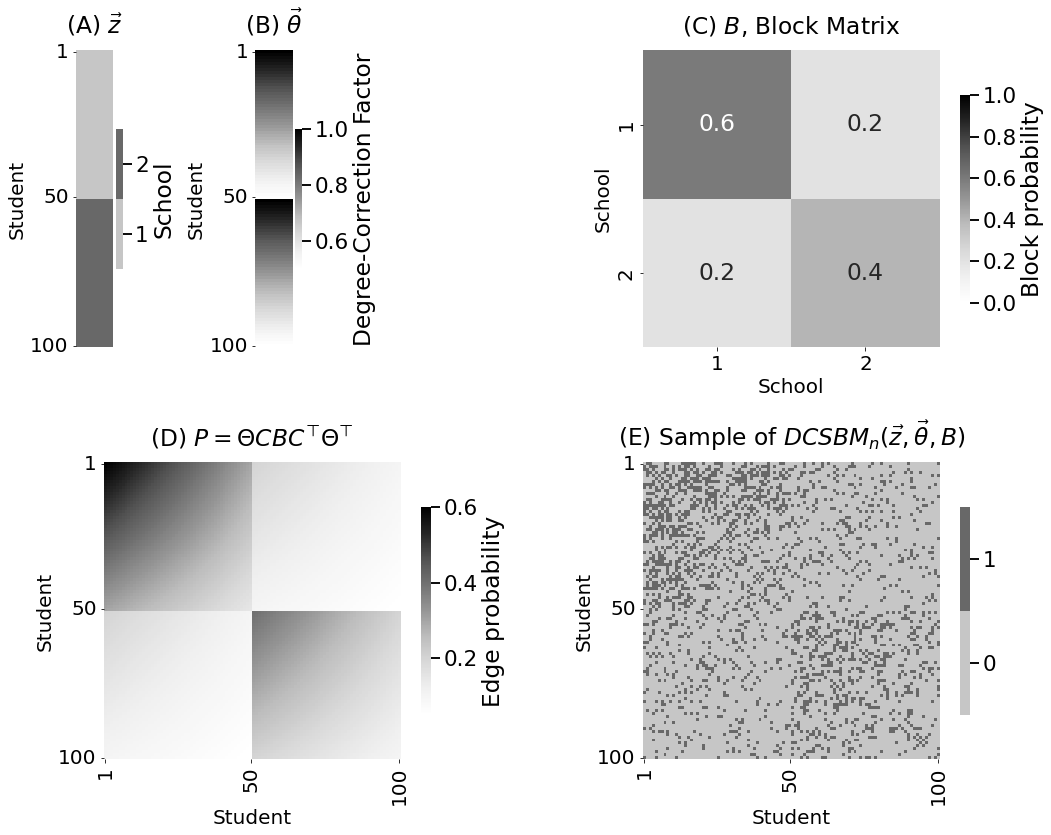
\includegraphics[width=0.9\linewidth]{representations/ch5/Images/dcsbm.png}
    \caption[Parameters of $DCSBM_n(\vec z, \vec \theta, B)$ random network]{\textbf{(A)} the community assignment vector, \textbf{(B)} the degree-correction vector, and \textbf{(C)} the block probability matrix. \textbf{(D)} the probability matrix, calculated from the community assignment vector, the degree-correction vector, and the degree-correction factor. \textbf{(E)} a sample from a $DCSBM_n(\vec z, \vec \theta, B)$ random network, using the probability matrix from \textbf{(D)} coupled with an $IER_n(P)$ network sampler from \texttt{graspologic}.}
    \label{fig:ch5:dcsbm}
\end{figure}

\subsection{Why is it called a degree-corrected stochastic block model?}

To begin to understand this, we will first think about the stochastic block model. Let's imagine that $\mathbf A$ is a $SBM_n(\vec z, B)$ random network with two communities. Let's imagine that the node $i$ is in community $1$, so $z_i = 1$. The expected node degree for a node $i$ in community $1$ can be written:
\begin{align*}
    \mathbb E[\mathbf d_i ; z_i = 1] &= \sum_{j \neq i} \mathbb E[\mathbf a_{ij}; z_i = 1] = \sum_{j \neq i}p_{ij}.
\end{align*}
All that the semicolon means is that we are proceeding with the assumption that we are calculating the expected degree for a node where $z_i = 1$ (the node $i$ is in community $1$, and $z$ is the vector denoting the community of each node). 

For the stochastic block model, this relationship is extremely simple. If node $i$ is in community $1$, this sum can be split into:
\begin{align*}
    \mathbb E[\mathbf d_i ; z_i = 1] &= \sum_{j : z_j = 2}p_{ij} + \sum_{j : z_j = 1\text{ and }j \neq i}p_{ij},
\end{align*}
So basically, we have split the sum into a sum over the other nodes in community $2$ (where $z_j = 2$) and the nodes that are not node $i$ but are also in community $1$. Note that for nodes in community $2$, $p_{ij} = b_{12}$. For nodes in community $1$, $p_{ij} = b_{11}$. Therefore:
\begin{align*}
    \mathbb E[\mathbf d_i ; z_i = 1] &= n_2 b_{12} + (n_1 - 1) b_{11}.
\end{align*}
Notice that nothing in the result here depends on the node, other than its community assignment. This means that for a $SBM_n(\vec z, B)$ random network, the nodes all have the same expected degree (if they are in the same community). This is known as the \textit{degree-homogeneity within-community} of the stochastic block model: all nodes (in the same community) have the same node expected node degree.

On the other hand, let's imagine that the network is a $DCSBM_n(\vec z, \vec \theta, B)$ random network. This expression gets a little more complicated, and becomes:
\begin{align*}
    \mathbb E[\mathbf d_i ; z_i = 1] &= \sum_{j \neq i} \mathbb E[\mathbf a_{ij}] = \sum_{j \neq i}\theta_i\theta_j p_{ij}.
\end{align*}
When we work through the same math as we showed above, this time we get:
\begin{align*}
    \mathbb E[\mathbf d_i ; z_i = 1] &= \theta_i \left(n_2 b_{12}\sum_{j : z_j = 2}\theta_j + (n_1 - 1) b_{11}\sum_{j : z_j = 1\text{ and }j \neq i}\theta_j\right),
\end{align*}
and the expected degree of the node $i$ is ``degree-corrected'' by its degree-correction factor $\theta_i$. 

\begin{floatingbox}[h]\caption{Concept: The expected node degree for block models}
\label{box:ch5:dcsbm:exp_deg}
If $\mathbf A$ is a $SBM_n(\vec z, B)$ random network with $n$ nodes and $K$ communities, then the expected degree of a node $i$ is:
\begin{align*}
    \mathbb E[\mathbf d_i ; z_i = k] &= \sum_{l \neq k} n_l b_{lk} + (n_k - 1)b_{kk}.
\end{align*}
If $\mathbf A$ is a $DCSBM_n(\vec z, \vec \theta, B)$ random network with $n$ nodes and $K$ communities, then the expected degree of a node $i$ is:
\begin{align*}
    \mathbb E[\mathbf d_i; z_i = k] &= \theta_i \left(\sum_{l \neq k}\left[n_l b_{lk}\sum_{j : z_j = l}\theta_j\right] + (n_k - 1)b_{kk}\sum_{j : z_j = k\text{ and }j \neq i}\theta_j\right).
\end{align*}
\end{floatingbox}

\newpage
\section{Positive Semi-Definite Block Matrices}
\label{sec:ch5:psd_block}

The primary difference between the $RDPG_n(X)$ and the $SBM_n(\vec z, B)$ or the $DCSBM_n(\vec z, \vec \theta, B)$ random networks boils down to a relatively obtuse mathematical concept: the semi-definiteness of the block matrix $B$ (or lackthereof). Remember that the block matrix $B$ is a $K \times K$ probability matrix (with one row/column for each of the $K$ communities).

We decided that a suitable definition of semi-definiteness of the block matrix for our purposes was that the block matrix $B$ could be decomposed into the product of another matrix, $\sqrt B$, with its transpose $\sqrt B^\top$. The matrix $\sqrt B$ is formally called the Gram matrix, which is common in matrix analysis \cite{Horn2012Oct}. For our purposes, understanding it to be the ``square-root matrix'' of the block matrix will suffice. While conceptualizing this result entirely is a bit beyond the scope of our book, we used this fact to conclude that a suitable ``test'' of when $B$ was positive semi-definite was a check that all of the eigenvalues of B were greater than or equal to 0:

\begin{lstlisting}[style=python]
import numpy as np

def is_psd(B):
    """
    A function which indicates whether a block matrix
    B is positive semi-definite.
    """
    return np.all(np.linalg.eigvals(B) >= 0)
\end{lstlisting}

Let's restrict ourselves precisely to the $2 \times 2$ case, in which we have two communities, so that we can build up some intuition for what a positive semi-definite block matrix looks like. In this case, the block matrix is:
\begin{align*}
    B &= \begin{bmatrix}
        b_{11} & b_{12} \\
        b_{21} & b_{22}
    \end{bmatrix},
\end{align*}

As it turns out, the existence of this square-root matrix in the $2 \times 2$ case can be summarized succinctly:
\begin{enumerate}
    \item $b_{11} \geq 0$, and
    \item the determinant of the block matrix is non-negative; that is, $det(B) \geq 0$.
\end{enumerate}
Since the block matrix $B$ is a probability matrix, condition one applies automatically, since a probability cannot be negative. 

Remembering back to linear algebra, the determinant of a $2 \times 2$ symmetric matrix $B$ is $b_{11}b_{22} - b_{21}^2$. This means that the block matrix will be positive semi-definite any time that $b_{11}b_{22} \geq b_{21}^2$. When a matrix has all positive entries but is not positive semi-definite, we refer to the matrix as \textit{indefinite}. It is necessary to clarify here that the matrices must have all positive entries for this result to hold, as there are several other classes of matrices involving their definiteness that cannot arise if we restrict to positive matrices.

To conceptualize what this means intuitively, we'll introduce some different classifications of SBMs. These are covered in more technical depth in \cite{Chung2021Mar}.

\subsection{Erd\"os-R\'enyi block matrix}

A block matrix is called \textit{Erd\"os-R\'enyi} if all entries are equal. In the $2 \times 2$ symmetric case, this means that $b_{11} = b_{22} = b_{12}$. It should be pretty obvious to you that if $B$ has only one unique entry, and $\vec z$ is any community assignment vector, that the resulting probability matrix will have $1$ unique entry too, which is equivalent to the probability matrix for an $ER_n(p)$ network where $p$ is chosen to be equal to the unique entry of $B$. 

Since we already showed that $ER_n(p)$ random networks were $RDPG_n(X)$, and $RDPG_n(X)$ can only have probability matrices that are positive semi-definite, we've already established that this $B$ matrix must be positive semi-definite. 

To see it formally, notice that $b_{11} = b_{22} = b_{12}$ implies that $b_{11}b_{22} = b_{12}^2$, so the determinant of $B$ is non-negative.

\subsection{Homophilic block matrices}
\label{sec:ch5:psd_block:homophily}

A block matrix is called \textit{homophilic} when the diagonal entries, $b_{kk}$ for all communities $k$, are greater than the off-diagonal entries $b_{kl}$ where $k \neq l$. In a rough definition, ``homophilic'' means tending to form relationships with people similar to oneself. In the context of a network, this means that the nodes of a SBM with a homophilic block matrix are more probable to have connections with nodes from the same community than with different communities.

Homophilic block matrices are positive semi-definite in general. We can see this very easily for the $2 \times 2$ case using the determinant condition for $B$. Notice that since $b_{11}$ and $b_{22}$ are each greater than $b_{21}$ and are non-negative, their product will be greater than $b_{21}^2$. 

Next, let's generate and plot a homophilic block matrix, so that we can start to get some intuition building up:

\begin{lstlisting}[style=python]
import numpy as np
from graphbook_code import heatmap

B = np.array([[0.6, 0.2], 
              [0.2, 0.4]])
heatmap(B, title="A homophilic block matrix", annot=True)
is_psd(B)
# True
\end{lstlisting}

This figure is shown in Figure \ref{fig:ch5:psd_bmtx}(A).

\begin{figure}[h]
    \centering
    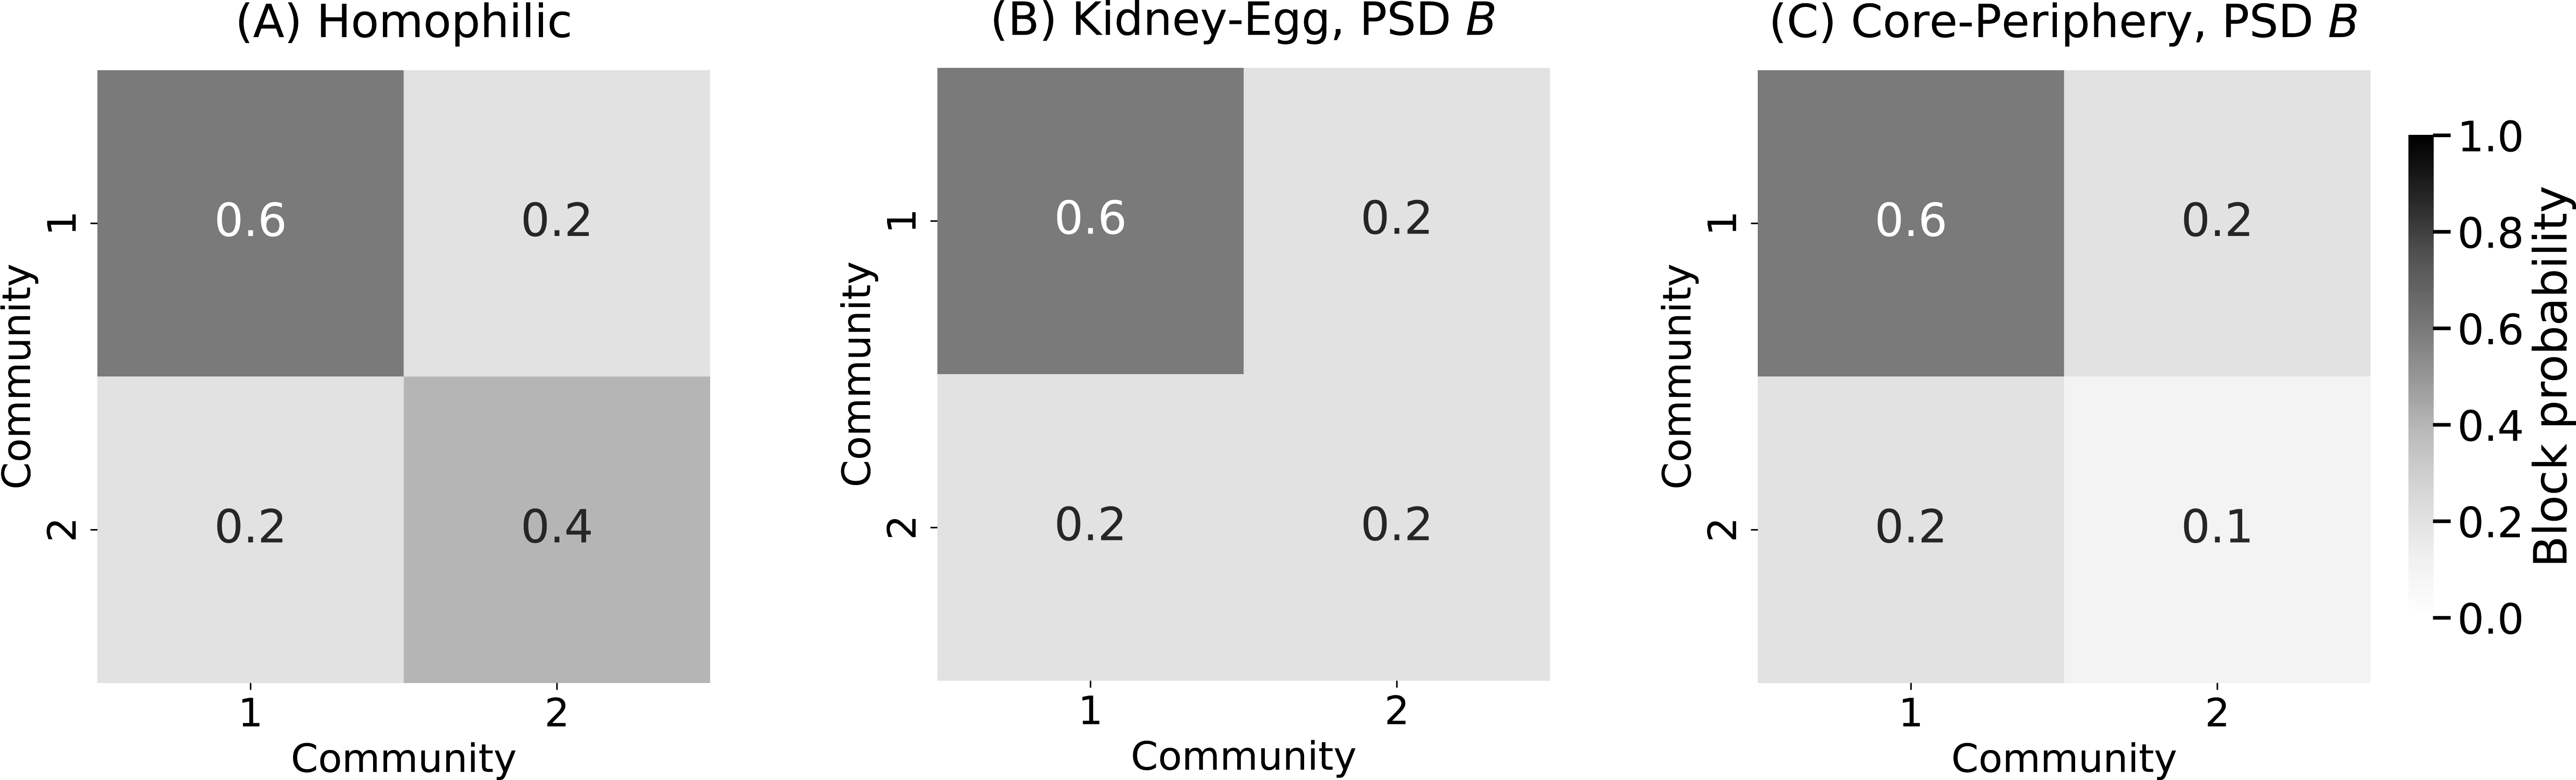
\includegraphics[width=\linewidth]{representations/ch5/Images/psd.png}
    \caption[PSD block matrices]{\textbf{(A)} a homophilic block matrix. \textbf{(B)} a positive semi-definite kidney-egg block matrix. \textbf{(C)} a positive semi-definite core-periphery block matrix.}
    \label{fig:ch5:psd_bmtx}
\end{figure}

\subsection{Planted partition block matrices}

A \textit{planted partition} block matrix is a block matrix where all of the on-diagonal entries are equal; that is, $b_{11} = b_{22} = \hdots = b_{KK}$ for all $K$ communities, and all of the off-diagonal entries are equal; that is, $b_{12} = \hdots b_{1K} = b_{21} = \hdots b_{2K} = \hdots b_{K1} = \hdots = b_{KK-1}$. In our case, this just means that $b_{11} = b_{22}$. 

Using the determinant condition and the fact that $b_{11} = b_{22}$, this implies that a planted partition is symmetric when $b_{11}^2 \geq b_{12}^2$. Since the entries of $B$ are probabilities and are hence non-negative, we can take square roots of both sides, and a sufficient condition is that $b_{11} \geq b_{12}$. When this criterion is satisfied, further clarify that the planted partition is a homophilic planted partition, because it fulfills the homophily criterion given in Section \ref{sec:ch5:psd_block:homophily}. 

We can generate an indefinite planted partition block matrix by just making an example where the block matrix has off-diagonal entries that exceed the on-diagonal entries, like this:


\begin{lstlisting}[style=python]
B_indef = np.array([[.1, .2], 
                    [.2, .1]])
is_psd(B_indef)
# False
\end{lstlisting}

\begin{figure}[h]
    \centering
    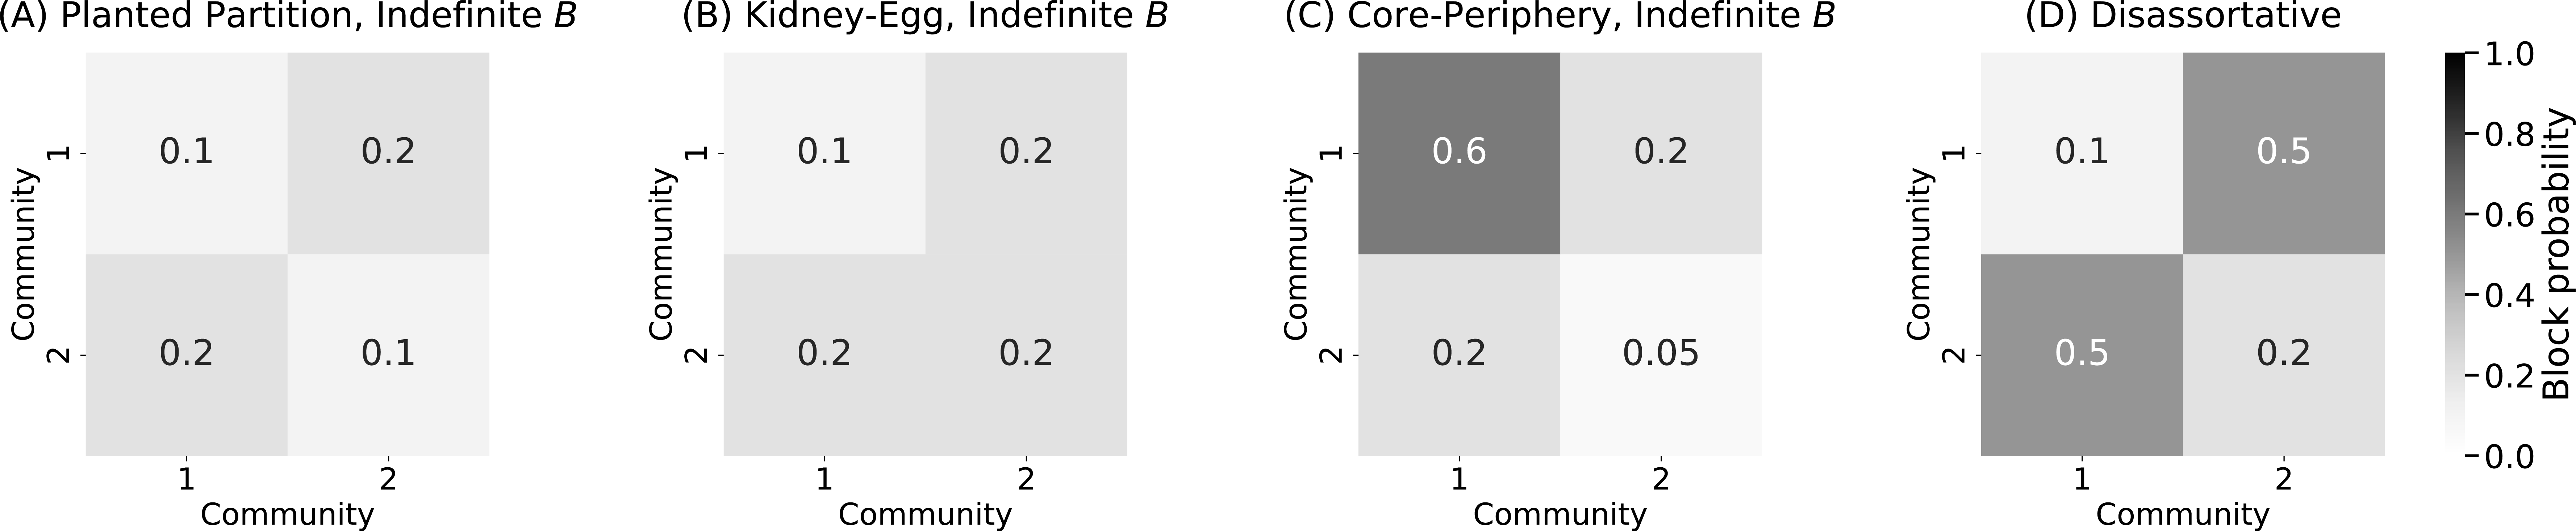
\includegraphics[width=\linewidth]{representations/ch5/Images/indef.png}
    \caption[Indefinite block matrices]{\textbf{(A)} an indefinite planted partition block matrix. \textbf{(B)} an indefinite kidney-egg block matrix. \textbf{(C)} an indefinite core-periphery block matrix. \textbf{(D)} a disassortative block matrix.}
    \label{fig:ch5:indef_bmtx}
\end{figure}

Which is shown in Figure \ref{fig:ch5:indef_bmtx}(A).

\subsection{Kidney-egg block matrices}

A \textit{kidney-egg} block matrix is a $2 \times 2$ block matrix where $b_{12} = b_{21} =  b_{22}$. For this matrix to be positive semi-definite, the determinant condition along with $b_{12} = b_{21} = b_{22}$ gives us that $b_{11}b_{12} \geq b_{12}^2$. Dividing through by $b_{12}$, we can see that the kidney-egg block matrices are positive semi-definite with the same conditions as planted partition block matrices; that is, $b_{11} \geq b_{12}$. Next, we generate two kidney-egg block matrices, one of which is indefinite and one of which is positive semi-definite. 

\begin{lstlisting}[style=python]
# a positive semi-definite kidney-egg block matrix
B_psd = np.array([[.6, .2], 
                  [.2, .2]])
is_psd(B_psd)
# True

# an indefinite kidney-egg block matrix
B_indef = np.array([[.1, .2], 
                    [.2, .2]])
is_psd(B_indef)
#False
\end{lstlisting}

We plot the positive semi-definite matrix in Figure \ref{fig:ch5:psd_bmtx}(B), and the indefinite matrix in Figure \ref{fig:ch5:indef_bmtx}(B).

\subsection{Core-periphery block matrices}

Core-periphery block matrices are block matrices where either $b_{11}$ or $b_{22}$ are greater than all of the other entries of the block matrix. This is called the core-periphery model because there are a group of nodes from a particular community (the \textit{core}) that tend to much more strongly connected than nodes that are not in that community (the \textit{periphery}). For instance, if community $1$ were the core community, $b_{11} > b_{22}$ and $b_{11} > b_{12}$, so the nodes of community $1$ tend to heavily associate with other core nodes. However, the nodes of community $2$ (the peripheral community) have far fewer connections both with other peripheral nodes and with core nodes. 

Core-periphery block matrices are a little bit harder to tie directly to positive semi-definiteness; the most precise that we can be is simply to say that $b_{11}b_{22} \geq b_{12}b_{21}$, which isn't particularly informative since that's literally the criterion for positive semi-definiteness that we gave.

Let's show how this condition works with some more examples:


\begin{lstlisting}[style=python]
# a positive semi-definite core-periphery block matrix
B_psd = np.array([[.6, .2], 
                  [.2, .1]])
is_psd(B_psd)
# True

# an indefinite core-periphery block matrix
B_indef = np.array([[.6, .2], 
                    [.2, .05]])
is_psd(B_indef)
# False
\end{lstlisting}

The positive semi-definite core-periphery block matrix is shown in Figure \ref{fig:ch5:psd_bmtx}(C), and the indefinite core-periphery block matrix is shown in Figure \ref{fig:ch5:indef_bmtx}(C).

\subsection{Disassortative block matrices}

A block matrix is \textit{disassortative} if $b_{12}$ and $b_{21}$ are greater than $b_{11}$ and $b_{22}$. By definition, disassortative block matrices are not positive semi-definite. This is because $b_{11}b_{22} < b_{12}b_{21}$, since all of the entries of $B$ are positive, and using the definition of the disassortative condition. Disassortative block matrices are a big conceptual ``thorn'' in the side of $RDPG_n(X)$ networks, as there is no possible way that we could use a disassortative block matrix to construct an equivalent $RDPG_n(X)$. 

To conceptualize what this would mean for a network, let's imagine that we have a simple network where the nodes are businesses, and each node is either a producer or a retailer. An edge exists in the network if a business relationship exists between two businesses. In general, producers will have business relationships with retailers, so the cross-community block probability $b_{12}$ is high. However, producers will not tend to have business relationships with their competitor producers, and retailers will not tend to have business relationships with their competitor retailers, so the within-community block probabilities $b_{11}$ and $b_{22}$ are comparatively low.

We can generate a disassortative block probability matrix like this:
\begin{lstlisting}[style=python]
# an indefinite disassortative block matrix
B = np.array([[.1, .5], 
              [.5, .2]])
is_psd(B)
# False
\end{lstlisting}

A plot of an indefinite block matrix is shown in Figure \ref{fig:ch5:indef_bmtx}(D), and another example of a disassortative block matrix would be the indefinite planted partition block matrix shown in Figure \ref{fig:ch5:indef_bmtx}(B).

\subsection{How do we generate latent position matrices for $SBM_n(\vec z, B)$ random networks which are positive semi-definite?}
\label{sec:ch5:psd_block:lpm_fromsbm}
When a real matrix $W$ is positive semi-definite, as we mentioned, we can obtain a square-root matrix $\sqrt W$ where $W = \sqrt{W}\sqrt{W}^\top$. This matrix can be generated through a process known as the {Cholesky Decomposition} \cite{Horn2012Oct}. This process will come in handy over the next few sections when we are dealing with SBM block matrices and probability matrices that are positive semi-definite, and we want to obtain a latent position matrix. You can do this with \texttt{numpy}, like so:

\begin{lstlisting}[style=python]
# homophilic, and hence positive semi-definite, block matrix
B = np.array([[0.6, 0.2], 
              [0.2, 0.4]])

# generate square root matrix
sqrtB = np.linalg.cholesky(B)

# verify that the process worked through by equality element-wise
# use allclose instead of array_equal because of extremely tiny
# numerical precision errors
np.allclose(sqrtB @ sqrtB.T, B)
# True
\end{lstlisting}

Next, we'll generate a community-assignment vector, and then use the code that we first produced in Section \ref{sec:ch5:ier:sbm_pmtx} to obtain a one-hot-encoding of the community-assignment vector. We can then use that to produce a latent position matrix, using the instructions from Equation \eqref{eq:ch5:ier:sbm_rdpg}, by taking $X = C\sqrt B$:

\begin{lstlisting}[style=python]
from graphbook_code import ohe_comm_vec

def lpm_from_sbm(z, B):
    """
    A function to produce a latent position matrix from a
    community assignment vector and a block matrix.
    """
    if not is_psd(B):
        raise ValueError("Latent position matrices require PSD block matrices!")
    # one-hot encode the community assignment vector
    C = ohe_comm_vec(z)
    # compute square root matrix
    sqrtB = np.linalg.cholesky(B)
    # X = C*sqrt(B)
    return C @ sqrtB

# make a community assignment vector for 25 nodes / community
nk = 25
z = np.repeat([1, 2], 25)

# latent position matrix for an equivalent RDPG
X = lpm_from_sbm(z, B)
\end{lstlisting}

The resulting latent position matrix is shown along with the community assignment vector and the block matrix in Figure \ref{fig:ch5:psd_block:sbm_lpm}.

\begin{figure}[h]
    \centering
    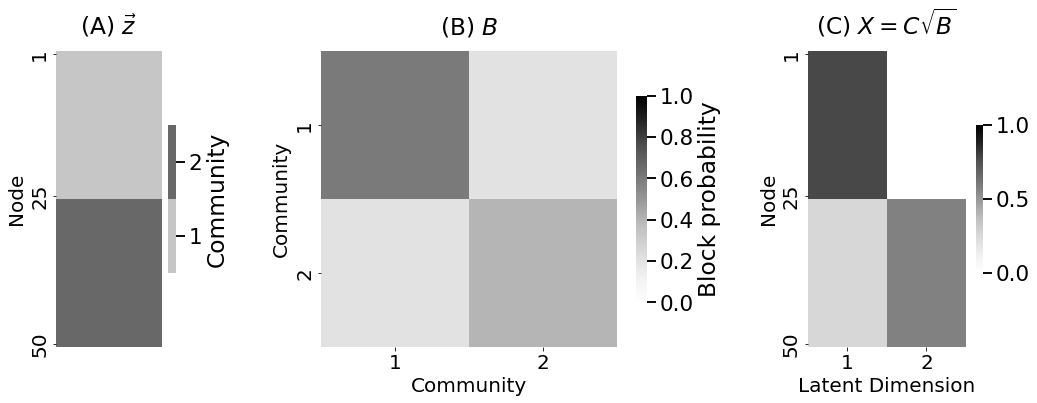
\includegraphics[width=\linewidth]{representations/ch5/Images/sbm_lpm.png}
    \caption[Latent position matrix for a positive semi-definite SBM]{\textbf{(A)} the community-assignment vector. \textbf{(B)} a homophilic block matrix, which is positive semi-definite. \textbf{(C)} the latent positions for an equivalent RDPG. Note that nodes with the same community have the same latent positions (rows of the latent position matrix $X$ in \textbf{(C)}).}
    \label{fig:ch5:psd_block:sbm_lpm}
\end{figure}

Finally, we can verify that the latent position matrix and the process described in Section \ref{sec:ch5:ier:sbm_pmtx} to generate the probability matrix for an SBM produce the same probability matrix:

\begin{lstlisting}[style=python]
from graphbook_code import generate_sbm_pmtx

# generate the probability matrices for an RDPG using X and SBM
P_rdpg = X @ X.T
P_sbm = generate_sbm_pmtx(z, B)

# verify equality element-wise
np.array_equal(P_rdpg, P_sbm)
# True
\end{lstlisting}

We can build a similar utility for the $DCSBM_n(\vec z, \vec \theta, B)$ random network, using Section \ref{sec:ch5:dcsbm:rdpg}, like so:

\begin{lstlisting}
def lpm_from_dcsbm(z, theta, B):
    """
    A function to produce a latent position matrix from a
    community assignment vector, a degree-correction vector,
    and a block matrix.
    """
    # X' = C*sqrt(B)
    Xp = lpm_from_sbm(z, B)
    # X = Theta*X' = Theta * C * sqrt(B)
    return np.diag(theta) @ Xp

# make a degree-correction vector
theta = np.tile(np.linspace(1, 0.5, 25), 2)
X_dcsbm = lpm_from_dcsbm(z, theta, B)
\end{lstlisting}

The resulting latent position matrix is shown along with the community assignment vector, the degree-correction vector, and the block matrix in Figure \ref{fig:ch5:psd_block:dcsbm_lpm}.

\begin{figure}[h]
    \centering
    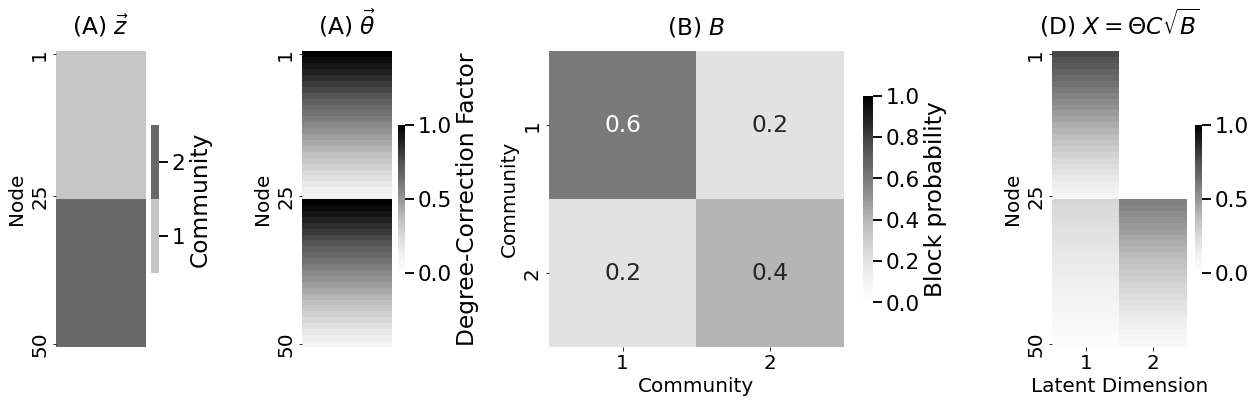
\includegraphics[width=\linewidth]{representations/ch5/Images/dcsbm_lpm.png}
    \caption[Latent position matrix for a positive semi-definite DCSBM]{\textbf{(A)} the community-assignment vector. \textbf{(B)} the degree-correction vector. \textbf{(C)} a homophilic block matrix, which is positive semi-definite. This block matrix is the same example shown in Figure \ref{fig:ch5:psd_bmtx}(A). \textbf{(D)} the latent positions for an equivalent RDPG. Note that nodes with the same community have similar latent positions, but appear to follow the same pattern in the degree-correction vector (large magnitudes for the first few nodes in each community, and smaller magnitudes for the last few nodes in each community).}
    \label{fig:ch5:psd_block:dcsbm_lpm}
\end{figure}

\subsection{Nodes in the same community (and with the same degree-correction factor) have the same latent position}
\label{sec:ch5:psd_block:same_lp}

As we learned in Equation \eqref{eq:ch5:ier:sbm_rdpg}, an $SBM_n(\vec z, \vec \theta, B)$ random network with a positive semi-definite block matrix (and hence a positive semi-definite probability matrix) can be represented as an $RDPG_n(X)$ random network, where the latent position matrix is:
\begin{align*}
    X = C \sqrt B
\end{align*}
For simplicity's sake, let's imagine that our SBM random network has two communities, and let's imagine the node $i$ is in community $1$. This means that the first row of the latent position matrix will be:
\begin{align*}
    \vec x_i^\top = \begin{bmatrix}
        1 & 0
    \end{bmatrix}\sqrt B.\numberthis \label{eqn:psd_block:c1}
\end{align*}
Now, let's imagine that we have another node, $i'$, which is also in community $1$. What is its latent position matrix?

That's right, you guessed it: it's the {exact same thing}, because the only thing that conveys information here is which community the node is in (which determines its row of the matrix $C$). What about a node $j$ in community $2$? This node will have a latent position of:
\begin{align*}
    \vec x_j^\top = \begin{bmatrix}
        0 & 1
    \end{bmatrix}\sqrt B. \numberthis \label{eqn:psd_block:c2}
\end{align*}
What would be the latent position vector for another node $j'$ also in community $2$? Again, it's the same thing. We could repeat this process for arbitrarily many communities; we just used the $2$-community case for simplicity. This example is shown in Figure \ref{fig:ch5:psd_block:sbm_lpm}(C). Notice that the rows of the latent position matrix (the latent positions for each node) are the same for nodes of the same community.

You can generalize this pattern to {any} nodes in the same community for an $SBM_n(\vec z, B)$ random network with a positive semi-definite block matrix: they will {always} have the same latent position vectors. 

We show an example of a homophilic block matrix in Figure \ref{fig:ch5:psd_block:sbm_lpm}(A), which you learned above is positive semi-definite because it is homophilic. When we apply the conversion utility \texttt{lpm\_from\_sbm()}, we produce the latent position matrix in Figure \ref{fig:ch5:psd_block:sbm_lpm}(C). Notice that the rows for each of the two communities are equal. 

This insight provides us with the answer to the side note that we mentioned in Section \ref{sec:ch5:ier:rdpg_sbm}, that the street example provided a counter example indicating that not all $RDPG_n(X)$ random networks can be represented as $SBM_n(\vec z, B)$ random networks. For the street example, all of the latent positions are different for each node. If it were possible to represent the street example as an $SBM_n(\vec z, B)$ random network with $K < n$ communities, there would need to exist a group of nodes with the same latent position vector.

For a $DCSBM_n(\vec z, \vec \theta, B)$ random network, it's a little bit less clear what will happen. You learned in Section \ref{sec:ch5:dcsbm:rdpg} that the latent position matrix for a $DCSBM_n(\vec z, \vec \theta, B)$ when the block matrix (and hence also the probability matrix) was positive semi-definite was:
\begin{align*}
    X &= \Theta C \sqrt B.
\end{align*}
Intuitively, this feels very similar to the situation for the $SBM_n(\vec z, B)$ random network case, and it is.

Since $\Theta_i$ is diagonal, we can easily study what happens when you multiply $\Theta$ and $C$ together. It ends up working out like this:

\begin{align*}
    \Theta C &= \begin{bmatrix}
        \theta_1 c_{11} & \hdots & \theta_1 c_{1K} \\
        \vdots & \ddots & \vdots \\
        \theta_n c_{n1} & \hdots & \theta_n c_{nK}
    \end{bmatrix}
\end{align*}

All that you will end up doing is rescaling each row of $C$ (which was the one-hot encoding for each individual node's community assignment) by that node's degree-correction factor. Let's work back through the two community example as before, where $B$ is positive semi-definite (and hence, $\sqrt B$ exists). 

The latent position for a node $i$ in community $1$ is:
\begin{align*}
    \vec x_i^\top &= \begin{bmatrix}
        \theta_i & 0
    \end{bmatrix} \sqrt B,
\end{align*}
and for another node $i'$ also in community $1$ is:
\begin{align*}
    \vec x_{i'}^\top &= \begin{bmatrix}
        \theta_{i'} & 0 
    \end{bmatrix}\sqrt B.
\end{align*}

These two vectors are identical when $\theta_i = \theta_{i'}$. So, in some sense, the degree-correction factors $\theta_i$ or $\theta_{i'}$ are {rescaling} the latent position associated with community $1$ (which was given by Equation \ref{eqn:psd_block:c1}) for the node-specific latent position. 

Repeating this same process for two nodes $j$ and $j'$ in community $2$, we would get that:
\begin{align*}
    \vec x_j^\top &= \begin{bmatrix}
        0 & \theta_j
    \end{bmatrix} \sqrt B, \\
    \vec x_{j'}^\top &= \begin{bmatrix}
        0 & \theta_{j'} 
    \end{bmatrix}\sqrt B.
\end{align*}

Again, these two vectors are identical when $\theta_j = \theta_{j'}$. The degree-correction factors $\theta_i$ and $\theta_{j'}$ are {rescaling} the latent position associated with community $2$ (which was given by Equation \ref{eqn:psd_block:c2}) for the node-specific latent position. In this sense, we can conceptualize the degree-correction factor (with a positive semi-definite block matrix) as {rescaling} the latent position associated with a the community of that node. 

 This example is shown in Figure \ref{fig:ch5:psd_block:dcsbm_lpm}(D). Notice that the rows of the latent position matrix (the latent positions for each node) follow the same pattern (in magnitude) of the degree-correction vector in Figure \ref{fig:ch5:psd_block:dcsbm_lpm}(B). This is no accident: the degree-correction vector is  {rescaling} the latent position associated with the particular community.

 Even though the $DCSBM_n(\vec z, \theta, B)$ random networks are more complicated than the $SBM_n(\vec z, B)$ random networks due to the degree-correction factor, this still shows us that there are some $RDPG_n(X)$ random networks which cannot be represented as $DCSBM_n(\vec z, \theta, B)$ random networks with $K < n$. Working back to the street example again, there is no choice of degree-correction factors $\vec \theta$ which would allow us to rescale the latent position associated with a community and obtain the latent positions in the street example. Intuitively, you can conceptualize this result by noticing that the values of the latent dimensions from Figure \ref{fig:ch5:rdpg} for the street example have a pattern of taking opposites: as the value in latent dimension one increases, the value in latent dimension two decreases, and vice-versa (where all values of the latent position matrix were positive). Accounting for this with a degree-correction factor would require at a minimum that the pattern is the same; both would have to be simultaneously increasing or decreasing due to the fact that the latent position matrix has only positive entries.
 
So, we learned two things here:
\begin{enumerate}
    \item When the underlying random network is an $SBM_n(\vec z, B)$ and the block matrix is positive semi-definite, all nodes associated with the same community have the same latent position vector.
    \item When the underlying random network is an $DCSBM_n(\vec z, \vec \theta, B)$ and the block matrix is positive semi-definite, all nodes associated with the same community have the same latent position vector up to a rescaling by their degree-correction factor. If the nodes are in the same community and the degree-correction factor is the same, the nodes have the same latent position.
\end{enumerate}

\subsection{Some Thought Exercises}

This section should give you some good intuition on which block matrices are positive semi-definite in simple $2 \times 2$ cases. To solidify these concepts, we would strongly recommend that you go through the following exercises on your own:

\begin{enumerate}
    \item Choose a number of nodes $n$, and produce a community assignment vector to one of two communities for each of the $n$ nodes.
    \item Use the procedure that we outlined in Algorithm \ref{alg:ch5:sbm_pmtx} to generate a probability matrix for a given block matrix. Visualize the probability matrix, the adjacency matrix heatmap, and a layout plot of the networks alongside one another. 
    \item Generate a valid degree correction vector for the $n$ nodes. Use the procedure that we outlined in Algorithm \ref{alg:ch5:dcsbm_prob} to produce a probability matrix for the network, and generate a sample from the random network. Produce the same visualizations as above.
\end{enumerate}

\begin{floatingbox}[h]\caption{Core-periphery SBM and planted partition DCSBM equivalence}
Imagine that you have a $DCSBM_n(\vec z, \vec \theta, B)$, where the block matrix $B$ is a planted partition, and the degree-correction vector $\vec \theta$ has two unique values $u$ and $v$. These unique values are chosen such that whenever $z_i = 1$, $\theta_i = u$, and whenever $z_i = 2$, $\theta_i = v$. 
\begin{enumerate}
    \item Generate a visualization of the probability matrix.
    \item Use this visualization of the probability matrix to deduce that there exists a core-periphery block matrix $B'$ where $SBM_n(\vec z, B')$ and $DCSBM_n(\vec z, \vec \theta, B)$ have the same probability matrix.
    \item Find a function of $u$,$v$, and $B$ such that $B' = f(u, v, B)$. 
\end{enumerate}
Conclude that planted-partition DCSBMs with the degree-correction vector generated as-described are equivalent to core-periphery SBMs with a suitably chosen block matrix.
\end{floatingbox}
\newpage

\begin{floatingbox}[h]\caption{Exercise: Degree-correction factors ``stretch'' latent positions}
\label{box:ch5:psd_block:stretch}
Take a positive semi-definite block matrix $B$ associated with a $2$-community $SBM_n(\vec z, B)$ random network (for instance, the homophilic block matrix we used in the examples here). Take a range of values for $\theta$, from $0$ to $1$ in $0.1$ increments, and compute the latent position matrix for the $SBM_n(\vec z, B)$ random network. This will give you a $n \times 2$-dimensional latent position matrix.
\begin{enumerate}
    \item Take the latent position associated with community $1$ (it will be the same for all nodes in community $1$, and will be a $2$-dimensional point $\vec x$). Rescale it for all values of $\theta$. 
    \item Next, plot $\theta \vec x$, for all values of $\theta$. 
    \item Conclude that $\theta$ is ``stretching'' $\vec x$ along a straight line.
    \item Repeat for the latent position $\vec y$ associated with community $2$.
\end{enumerate}
Conclude that degree-correction factors for $DCSBM_n(\vec z, \vec \theta, B)$ random networks``stretch'' the latent positions of $SBM_n(\vec z, B)$ random networks along a straight line, depending on the value of $\theta$. 
\end{floatingbox}
\section{Structured Independent-Edge Random Network}
\label{sec:ch5:siem}

Next up, we'll cover a statistical model for networks which generalizes the SBM from Section \ref{sec:ch5:sbm} a little differently than the IER network from Section \ref{sec:ch5:ier}. Sometimes in a network, there might particular pairs of nodes which, when those nodes are incident a particular edge, impart a different distribution for that edge. Let's consider an example, which boils back to the example that we gave in Chapter \ref{sec:ch2}. Imagine we have a network where the $n=100$ nodes are different areas of the brain.  Each of these nodes are either in the left or the right side of the brain. An edge exists or does not exist if the two areas of the brain tend to be active together while a person interacts with the world. A common hypothesis in this scenario is that even though the left and right sides of the brain tend to have different functions, the nodes on the left and right sides still might tend to be active together, especially when it is the same region on both sides. 

For instance, even though the motor cortex (responsible for {motion} and {conscious movement}) in the left hemisphere has a slightly different function than the motor cortex in the right hemisphere, the two hemispheres tend to work together. The right motor cortex provides movement for the left side of the body, and the left motor cortex provides movement for the right side of the body. When someone is moving around, a lot of tasks will require them to use both sides of the body in tandem, so even though the two motor cortices are doing different jobs, they still tend to be active together. This pattern, known as \textit{bilateral homotopy}, trickles down to many other areas in the brain as well. Let's turn this into a question: do bilateral node pairs have higher connectivity than non-bilateral node pairs?

To answer this question, we need statistical models which capture what we understand about the system. Perhaps the edges between pairs of nodes which are bilaterally symmetric tend to be more likely than the edges between pairs of nodes which are not bilaterally symmetric. Based on what we know so far, we could achieve this property with an $IER_n(P)$ random network: Allow every pair of nodes in the network to have their own edge probability.

If we wanted to use our data (one network, with an adjacency matrix $A$) to describe this system, we are at a loss. On one hand, our network model is much simpler than a model which ascribes probabilities to every possible network configuration for an $n$ node simple network (of which there are $2^{\binom n 2}$, as-per Remark \ref{box:ch5:whyuse}). On the other, this model still has $\binom n 2$ parameters (the entries of the probability matrix $P$), one for each individual edge in the network. This is, in a sense, still exactly equivalent to the coin flipping problem from Remark \ref{box:ch5:whyuse}: to learn about a probability $p_{ij}$, we have exactly one edge $a_{ij}$. Learning about $p_{ij}$ from a single edge $a_{ij}$ is exactly as pointless as trying to learn about the probability a coin lands on heads from the outcome of a single coin toss. We need a better model.

Instead, we will conceptualize this problem a little bit differently using the Structured Independent Edge Model (SIEM).
\subsection{The Structured Independent Edge Model is parametrized by a Cluster-Assignment Matrix and a probability vector}
\subsubsection{The Cluster-Assignment Matrix}

The cluster assignment matrix $D$ is an $n \times n$ matrix which assigns potential edges in the random network to clusters. What do we mean by this?

Remember that the adjacency matrix $\mathbf A$ for a random network is {also} an $n \times n$ matrix, where each entry $\mathbf a_{ij}$ is a random variable which takes the value $0$ or the value $1$ with a particular probability. The cluster assignment matrix takes each of these $n^2$ random variables, and uses a parameter $v_{ij}$ to indicate which of $K$ possible clusters this edge is part of. In the brain example above, for instance, we could take $v_{ij} = 1$ when the nodes $i$ and $j$ are bilateral pairs, and $v_{ij} = 2$ when the nodes $i$ and $j$ are not bilateral pairs. For simple networks, we'll also add the restriction that $v_{ij} = v_{ji}$ for all node pairs $i$ and $j$, and we'll leave $z_{ii}$ to be unassigned (a value of \texttt{NA}) since simple networks are loopless.

\subsubsection{The Probability vector}

The second parameter for the SIEM is a probability vector, $\vec p$. If there are $L$ edge clusters in the SIEM, then $\vec p$ is a length-$L$ vector. Each entry $p_l$ indicates the probablity of an edge in the $l^{th}$ cluster existing in the network. For example, $p_1$ indicates the probability of an edge in the first edge cluster, $p_2$ indicates the probability of an edge in the second edge cluster, so on and so-forth. In the brain example, for instance, $p_1$ would represent the probability of an edge between a pair of nodes that represent the same brain area in opposite hemispheres (bilateral pairs), and $p_2$ would represent the probability of an edge between a pair of nodes that are not bilateral pairs.

\subsection{Conceptualizing the SIEM}

Like usual, we will formulate the SIEM using our old coin flip example. We begin by obtaining $L$ coins, where the $k^{th}$ coin has a chance of landing on heads of $p_k$, and a chance of landing on tails of $1 - p_k$. For each entry $\mathbf a_{ij}$, we identify the corresponding cluster $v_{ij}$ that this edge is in. Remember that $v_{ij}$ takes one of $L$ possible values. We flip the $v_{ij}$ coin, and if it lands on heads (with probability $p_{v_{ij}}$), the edge exists, and if it lands on tails (with probability $1 - p_{v_{ij}}$) the edge does not exist.

If $\mathbf A$ is an SIEM random network with $n$ nodes, the cluster assignment matrix $D$, and the probability vector $\vec p$, we say that $\mathbf A$ is an $SIEM_n(D, \vec p)$ random network.

\subsubsection{How do we simulate samples from an $SIEM_n(D, \vec p)$ random network?}

The procedure in Algorithm \ref{alg:ch5:siem} will produce for us a network $A$, which has nodes and edges, where the underlying random network $\mathbf A$ is an $SIEM_n(D, \vec p)$ random network.

\begin{algorithm}[h]\caption{Simulating a sample from an $SIEM_n(D, \vec p)$ random network}
\label{alg:ch5:siem}
\SetAlgoLined
\KwData{$n$ a number of nodes\newline $D$ a matrix which assigns one of $L$ edge-clusters to each of the $n^2$ edges \newline $\vec p$ a $L$-dimensional probability vector for each edge-cluster}
\KwResult{The adjacency matrix of a sample from the random network.}

For each of the $L$ clusters, obtain $L$ total weighted coins, where the $k^{th}$ coin lands on heads with probability $p_k$ and tails with probability $1 - p_k$.

\For{$i$ in $1$:$n$}{
    \For{$j > i$}{
        Flip the $v_{ij}$ coin, and if it lands on heads, the corresponding entry in the adjacency matrix $a_{ij}$ is $1$. If it lands on tails, the coresponding entry in the adjacency matrix $a_{ij}$ is $0$. 

        Let $a_{ji}= a_{ij}$.
    }
}

\Return{$A$}
\end{algorithm}

Let's turn back to our network example we looked at. The first fifty nodes will be the areas in the left hemisphere of the brain, and the second fifty nodes will be the areas of the right hemisphere of the brain. The nodes will be sequentially ordered, so that the first node of the left is the first node of the right, so on and so forth, for all $50$ pairs of nodes. Further, programmatically, it is much easier to encode \texttt{NA} as $0$, so we fill the diagonal with $0$s. Since the network we are generating is simply, these entries won't matter for our sample that we generate anyways. We can generate a cluster assignment matrix like this:

\begin{lstlisting}[style=python]
import numpy as np

n = 100
D = np.ones((n, n))
for i in range(0, int(n/2)):
    D[int(i + n/2), i] = 2
    D[i, int(i + n/2)] = 2
np.fill_diagonal(D, 0)
\end{lstlisting}

We'll also visualize the cluster assignment matrix along with the hemisphere of each brain node:

\begin{lstlisting}[style=python]
from graphbook_code import heatmap

labels = np.repeat(["L", "R"], repeats=n/2)
heatmap(D.astype(int), title="Cluster assignment matrix", 
        inner_hier_labels=labels)
\end{lstlisting}

The cluster assignment matrix is shown in Figure \ref{fig:ch5:siem}(A). As we can see, there are several ``bands'' going across this matrix. The bands are the stripes moving diagonally across the cluster assignment matrix. The white band is the diagonal entries. Since the networks we are dealing with are simple, they are undirected, so we do not need to worry about the diagonal entries.

In the off-diagonal entries, we can see another band. This band consists of the bilateral pairs of nodes; remember that the first node of the left hemisphere was the same functional area of the brain, but just in the other hemisphere. Hence, these edges are "assigned" to cluster $2$. Remember that the nodes are organized such that the first $\frac{n}{2}$ nodes are area $1$ for hemisphere $L$, so on and so forth for all areas of the left hemisphere. Next, the remaining $\frac{n}{2}$ nodes corresponding area $1$ for hemisphere $R$, so on and so forth for all of the areas of the right hemisphere. Therefore, this pattern will manifest as an ``offset'' band, where the ``offset'' amount of offset is simply the number of nodes between area $u$ in hemisphere $L$ and area $u$ in hemisphere $R$ (which is $\frac{n}{2}$ nodes in total). 

The remaining off-diagonal entries are not bilateral pairs of nodes. These entries are assigned to cluster $1$.
 

Next, we need a probability vector for the two clusters of off-diagonal entries. We will arbitrarily say that there is a $0.8$ probability that an edge adjoining two bilateral pairs of nodes (cluster $2$) is connected, but a $0.1$ probability that an edge adjoining two non-bilateral pairs of nodes (edge cluster $1$) is connected:

\begin{lstlisting}[style=python]
from graphbook_code import siem

p = [0.1, 0.8]
A = siem(n, p, D)
heatmap(A.astype(int), title="$SIEM_n(D, \\vec p)$ sample", 
        inner_hier_labels=labels)
\end{lstlisting}

The adjacency matrix is plotted in Figure \ref{fig:ch5:siem}(B). Notice that the adjacency matrix reflects the same banding pattern of the cluster assignment matrix. 

\begin{figure}[h]
    \centering
    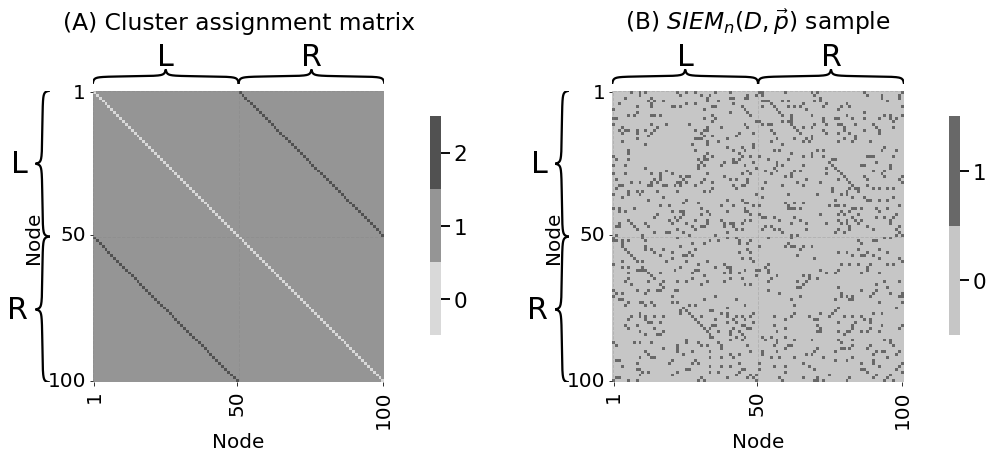
\includegraphics[width=\linewidth]{representations/ch5/Images/siem.png}
    \caption[Visualizing SIEM networks]{\textbf{(A)} the cluster assignment matrix $D$. \textbf{(B)} sample of an adjacency matrix from an $SIEM_n(D, \vec p)$ random network. }
    \label{fig:ch5:siem}
\end{figure}
\subsection{What is the relationship between the $SIEM_n(D, \vec p)$ random network and the $SBM_n(\vec z, B)$ random network?}

If you recall from Section \ref{sec:ch5:ier:ier_generalises}, we spent a lot of effort determining which networks were more complex than other networks. We can do this for the $SIEM_n(D, \vec p)$ random networks, too. 

We are going to demonstrate that every simple $SBM_n(\vec z, B)$ random network with $K < n$ communities can be represented as a simple $SIEM_n(D, \vec p)$ random network with $L < \binom n 2$ communities. The $SIEM_n(D, \vec p)$ with $L < \binom{n + 1}{2}$ is a similar level of complexity to the $SBM_n(\vec z, B)$ with $K < n$, because the block matrix for a $SBM_n(\vec z, B)$ with $K < n$ has less than $\binom{n + 1}{2}$ unique entries.

At an extremely high level, what we do is for each pair of communities $k$ and $k'$, we define a unique edge-cluster $l$. Next, for each pair of nodes $i$ and $j$, we check which communities they are part of, and then define $v_{ij}$ to be the edge cluster that corresponds to that pair of communities.

Finally, for the probability vector, we just take $p_l$ for a given edge-cluster $l$ to be the entry of $B$ whose indices mapped to edge-cluster $l$. For instance, if communities $k$ and $k'$ mapped to edge-cluster $l$, we take $p_l = b_{kk'}$. The resulting $SIEM_n(D, \vec p)$ random network has the same probability matrix as the $SBM_n(\vec z, B)$ random network, so all SBMs  with $K < n$ are SIEMs with $L < \binom{n + 1}{2}$.

The reverse is not true; the example provided here regarding bilateral brain areas is a counter example that cannot be represented using an $SBM_n(\vec z, B)$ random network with a number of communities $K < n$.

For this reason, the $SIEM_n(D, \vec p)$ with $L < \binom{n+1}{2}$ is more complex than the $SBM_n(\vec z, B)$ with $K < n$.

In later sections such as Section \ref{sec:ch7:testing}, we will develop statistical tools for $SIEM_n(D, \vec p)$ random networks, but it is important to note that they apply equally well to $SBM_n(\vec z, B)$ random networks. The statistical tools afforded to the SIEM will allow you to capture more general questions than those you could ask with just the SBM. The SIEM lets us find differences between pairs of groups of edges, rather than just looking for differences between pairs of groups of nodes, since there can be complicated arrangements of edges which are not easily capturable with the SBM.


\newpage
\section{Multiple Network Models}
\label{sec:ch5:multi}

Up to this point, we have studied network models which are useful for a single network. What should we do if we have multiple networks?

Let's imagine that a company with $100$ total employees. $25$ of these employees are company administrative executives (admin), $25$ of these employees are marketing experts (marketing), and $50$ of these employees are network machine learning experts (ml). You study the social media habits of your employees on Facebook, Twitter, and Linkedin. For a given social networking site, an edge is said to exist between a pair of employees if they are connected on the social media site (by being friends, following one another, or being connected, respectively). As it turns out, individuals tend to most closely associate with the colleagues whom they work most closely: you might expect some sort of community structure to your network, wherein network machine learning experts are more connected with network machine learning experts, marketing experts are more connected with marketing experts, so on and so forth. What we will see below is that all of the networks appear to have the same community organization, though on Linkedin, we see that the administrative executives tend to be a little more connected than the other team members. This is reflected in the fact that there are more connections between admin members on Linkedin and other team members. To do this, we'll use a homophilic stochastic block model from Section \ref{sec:ch5:psd_block} for the Facebook and Twitter networks, and a homophilic degree-corrected stochastic block model (with slightly fewer connections for non-admin team members, $\theta = 1$ and slightly more, $\theta=\sqrt 2$, for admin team members) for the Linkedin network. We will borrow the \texttt{dcsbm} function from Section \ref{sec:ch5:dcsbm}, and we'll borrow scikit-learn's LabelEncoder to encode our labels:

\begin{lstlisting}[style=python]
from graspologic.simulations import sbm
import numpy as np
from graphbook_code import dcsbm
from sklearn.preprocessing import LabelEncoder

# Create block probability matrix B
K = 3
B = np.full(shape=(K, K), fill_value=0.05)
np.fill_diagonal(B, 0.3)

# degree-correct the different groups
admin, marketing, ml = counts = [25, 25, 50]
theta = np.ones((np.sum(counts), 1))
theta[:admin, :] = np.sqrt(2)

# our dcsbm function only works with communities encoded 1,2,...,K
# so we'll use a LabelEncoder to map labels to integers
labels = np.repeat(["admin", "marketing", "ml",], counts)
le = LabelEncoder().fit(labels)
z = le.transform(labels)

# sample the random networks
A_facebook = sbm(n=counts, p=B)
A_twitter = sbm(n=counts, p=B)
A_linkedin, P_linkedin = dcsbm(z, theta, B, return_prob=True)
\end{lstlisting}

We illustrate heatmaps from each of the three networks in Figure \ref{fig:ch5:socialnets}. Notice that while the Facebook and Twitter networks do not look particularly different, the Linkedin network appears to show that administrative members tend to have much higher numbers of connections with other members.

\begin{figure}[h]
    \centering
    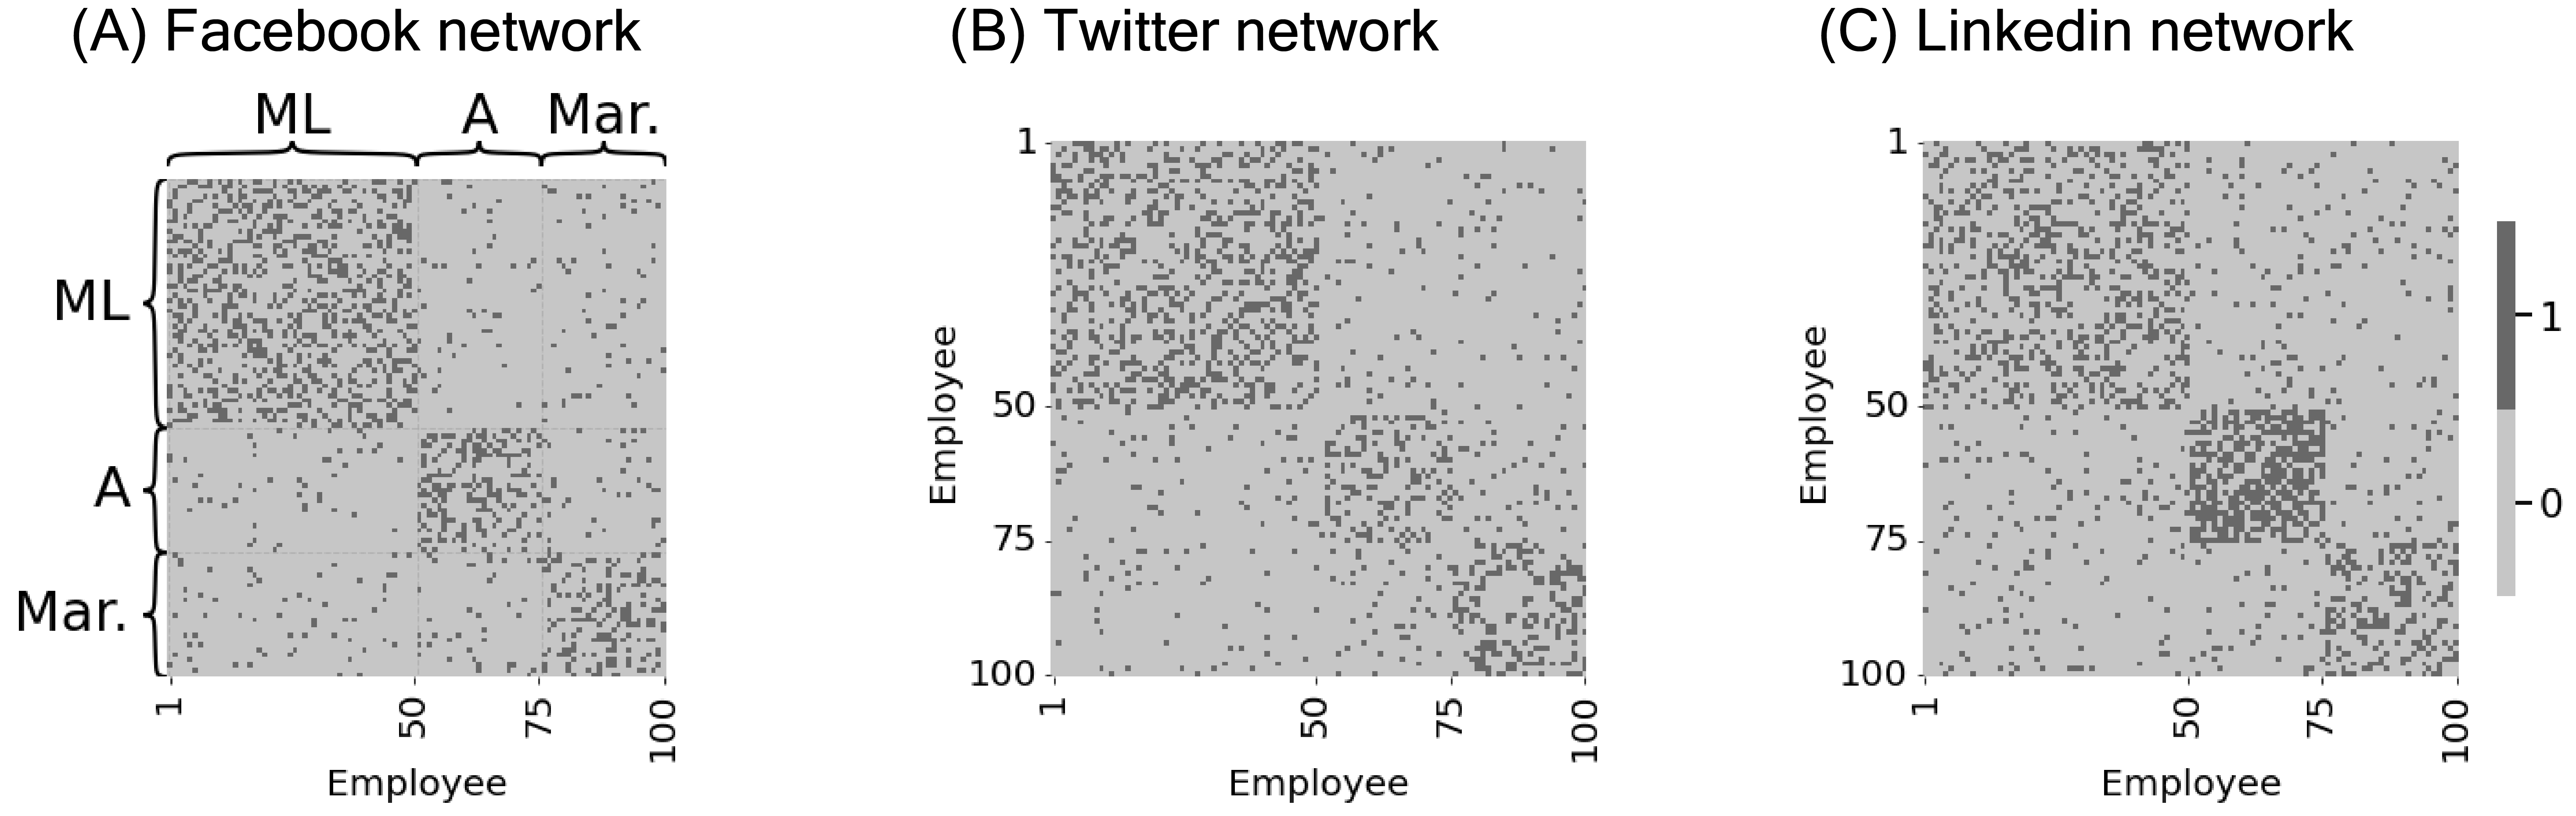
\includegraphics[width=\linewidth]{representations/ch5/Images/socialnets.png}
    \caption[Social networks for employees across Facebook, Twitter, and Linkedin.]{\textbf{(A)} Facebook social network. \textbf{(B)} Twitter social network. \textbf{(C)} Linkedin social network. Notice that on Linkedin, the administrators tend to have more edges.}
    \label{fig:ch5:socialnets}
\end{figure}

Remember that a random network has an adjacency matrix denoted by a boldfaced uppercase $\mathbf A$, and has network samples $A$ (which we just call "networks"). In our code, for example, the ``random network'' can be thought of as the sbm or dcsbm function itself -- and the "network" can be thought of as the adjacency matrix that you get when you call that function. When we have multiple networks, we will need to be able to index them individually. For this reason, in this section, we will use the convention that a random network's adjacency matrix is denoted by a boldfaced uppercase $\mathbf A^{(m)}$, where $m$ tells us which network in our collection we are talking about. The capital letter $M$ defines the \textit{total} number of random networks in your collection. 

In our social network example, since we have connection networks for $3$ sites, $M$ is $3$. When we use the letter $m$ itself, we will typically be referring to an arbitrary random network among the collection of random networks, where $m$ is between $1$ and $M$. When we have $M$ total networks, we will write down the entire {collection of random networks} using the notation $\left\{\mathbf A^{(1)}, ..., \mathbf A^{(M)}\right\}$. With what we already know, for a random network $\mathbf A^{(m)}$, we would be able to use a single nework model to describe $\mathbf A^{(m)}$. This means, for instance, if we thought that each social network could be represented by a different RDPG, that we would have a {different} latent position matrix $X^{(m)}$ to define each of the $30$ networks. What is the problem with this description?

What this description lacks is that the three networks share a {lot} of common information. We might expect that, on some level, the latent position matrices should also show some sort of common structure. This is because they each have the same block matrices, despite the fact that the Linkedin network incorporated a degree-correction factor for the administrative team.

However, since we used a {unique} latent position matrix $X^{(m)}$ for each random network $\mathbf A^{(m)}$, we have inherently stated that we think the networks have distinct latent position matrices. If we were to perform a task downstream, such as whether we could identify which employees are in which community, we would have to analyze each latent position matrix individually, and we would not be able to learn a latent position matrix with shared structure across the three networks. Before we jump into multiple network models, let's provide some context as to how we will build these up.

Moving forward, we'll tend to build off the Random Dot Product Graph (RDPG), and closely related variations of it. This is because of an idea we've been building up over the past several sections: the $RDPG_n(X)$ random networks can be used to describe all positive semi-definite $IER_n(P)$ networks. This means that using the RDPG gives you multiple random network models that will be inherently flexible. One of the models that we will discuss will use the ``generalized'' RDPG, the gRDPG \cite{Rubin2022Sep,Arroyo2021} as well, which will allow us to generalize to arbitrary $IER_n(P)$ networks. These models taken together are a powerful and unifying force across numerous disciplines of network machine learning, such as social networking, neuroscience, and many other fields.

\subsection{Joint Random Dot Product Graphs (JRDPG) Model}
\label{sec:ch5:multi:jrdpg}
In our social network example, notice that the Facebook and Twitter connections look qualitatively similar. It looks like they have relatively similar connectivity patterns between the different employee working groups, and we might even think that the underlying random network that governs these two social networks are {identical}. In statisical science, we use the term \textit{homogeneity} to describe a collection of $M$ random networks that have the same underlying random process. Let's put what this means into context using your coin flip example. If a pair of coins are \textit{homogeneous}, this means that the probability that they land on heads is identical. If we view edges as coinflips, this intuition extends directly to random networks. Let's get more clear with our definition of homogeneity.

\subsubsection{Homogeneous and heterogeneous collections of random networks}
A \textit{homogeneous} collection of independent-edge random networks $\left\{\mathbf A^{(1)}, ..., \mathbf A^{(M)}\right\}$ is one in which {all} of the $M$ random networks have the {same probability matrix}, and consequently have the same distribution (we use the term \textit{identically distributed} in statistics). Remember that the probability matrix $P^{(m)}$ is the matrix whose entries $p^{(m)}_{ij}$ indicate the probability that an edge exists between nodes $i$ and $j$. This is because the probability matrix is the fundamental unit which can be used to describe independent-edge random networks, as we learned in Section \ref{sec:ch5:ier}. On the other hand, a \textit{heterogeneous} collection of independent-edge random networks is a collection of networks $\left\{\mathbf A^{(1)}, ..., \mathbf A^{(M)}\right\}$ is one in which the probability matrices are {not} the same for all of the $M$ networks, and hence, they are {not} identically distributed. 

The probability matrices $P^{(1)}$ and $P^{(2)}$ for the random networks $\mathbf A^{(1)}$ and $\mathbf A^{(2)}$ for Facebook and Twitter from the example we introduced above are identical, because they have the same community assignment vector and the same block matrix. Since the probability for an $SBM_n(\vec z, B)$ random network is only a function of these two things as we saw in Algorithm \ref{alg:ch5:sbm_pmtx}, the probability matrices are the same.

\subsubsection{Conceptualizing the $JRDPG_{n,M}(X)$ model}

The Joint Random Dot Product Graphs (JRDPG) is the simplest way we can extend the RDPG random network model to multiple random networks. The way we can think of the JRDPG model is that for each of our $M$ total random neworks, the edges depend on a latent position matrix $X$. We say that a collection of random networks $\left\{\mathbf A^{(1)}, ..., \mathbf A^{(N)}\right\}$ with $n$ nodes is $JRDPG_{n,M}(X)$ if each random network $\mathbf A^{(m)}$ is $RDPG_n(X)$ and if the $M$ networks are independent. The joint random dot product graph model is formally described by \cite{Athreya2017Jan}, and has many connections with the omnibus embedding \cite{Levin2017}, which we will learn about in Section \ref{sec:ch6:multinet}.

\subsubsection{The JRDPG model does not allow you to heterogeneity}

Under the JRDPG model, each of the $M$ random networks share the same latent position matrix. Remember that for an RDPG, the probability matrix $P = XX^\top$. This means that for all of the $M$ networks, $P^{(m)} = XX^\top$ under the JRDPG model. hence, $P^{(1)} = P^{(2)} = ... = P^{(M)}$, and {all} of the probability matrices are {identical}! This means that the $M$ random networks are {homogeneous}. Consequently, the JRDPG can be thought of as $M$ homogeneous and independent RDPGs.

From Section \ref{sec:ch5:ier:sbm_pmtx}, we learned how to construct probability matrices from homophilic block matrices. Let's try this by generating the latent position matrices, using the process that we outlined in Section \ref{sec:ch5:ier:sbm_pmtx}:

\begin{lstlisting}[style=python]
from graphbook_code import generate_sbm_pmtx, heatmap

# we already returned P_li for the linkedin
# probability matrix from dcsbm() function
P_facebook_twitter = generate_sbm_pmtx(z, B)
# when plotting for comparison purposes, make sure you are
# using the same scale from 0 to 1
heatmap(P_facebook_twitter, vmin=0, vmax=1)
heatmap(P_linkedin, vmin=0, vmax=1)
heatmap(P_linkedin - P_facebook_twitter, vmin=0, vmax=1)
\end{lstlisting}

\begin{figure}[h]
    \centering
    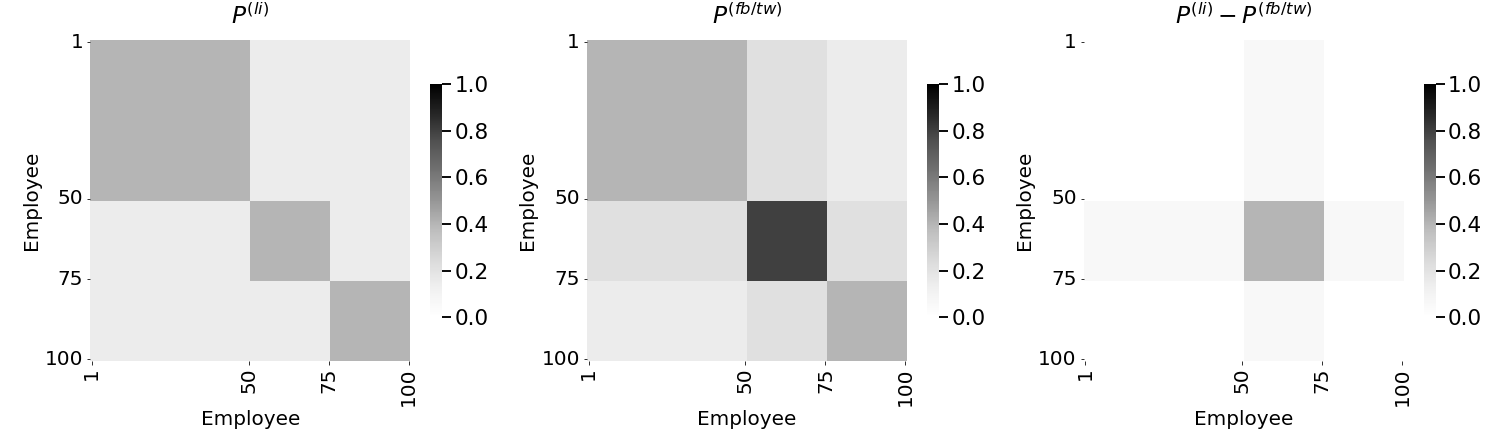
\includegraphics[width=\linewidth]{representations/ch5/Images/het.png}
    \caption[Heterogeneous random network probability matrices]{\textbf{(A)} the probability matrix for the random networks underlying twitter and facebook, $\mathbf A^{(1)}$ and $\mathbf A^{(2)}$. \textbf{(B)} the probability matrix for the random networks underlying linkedin. \textbf{(C)} the difference between the probability matrices for twitter/facebook and linkedin.}
    \label{fig:ch5:het}
\end{figure}
We illustrate heatmaps of the probability matrices in Figure \ref{fig:ch5:het}. Since the probability matrices for Facebook and Twitter in \ref{fig:ch5:het}(A) are exactly identical (they are both functions of the same block matrix $B$), the collection of random networks $\left\{\mathbf A^{(1)}, \mathbf A^{(2)}\right\}$ are homogeneous. We could model this pair of networks using the JRDPG due to their homogeneity and the fact that the underlying block matrices are homophilic (and hence, positive semi-definite with a positive semi-definite probability matrix).

On the other hand, $\mathbf A^{(1)}$ an $\mathbf A^{(2)}$ do not have the same probability matrix as $\mathbf A^{(3)}$, as shown in Figure \ref{fig:ch5:het}(B) and (C). This means that the collections of random networks $\left\{\mathbf A^{(1)}, \mathbf A^{(3)}\right\}$, $\left\{\mathbf A^{(2)}, \mathbf A^{(3)}\right\}$, and $\left\{\mathbf A^{(1)}, \mathbf A^{(2)}, \mathbf A^{(3)}\right\}$ are {heterogeneous}, because their probability matrices are different. 

So, unfortunately, the JRDPG cannot handle the hetereogeneity between the random networks of Facebook and Twitter with the random network for Linkedin. To remove this restrictive homogeneity property of the JRDPG, we can turn to a single network model that we just covered: the $IER_n(P)$ random network. Next, we will see how the IER random network can be used in conjunction with the COSIE model to allow you to capture this heterogeneity. 

\subsection{Common Subspace Independent Edge (COSIE) Model}
\label{sec:ch5:multi:cosie}

In our example on social networks, notice that the Facebook and Linkedin connections looked relatively similar, but had an important difference: on Linkedin, there was an administrative meeting, and the employees on the administrative team exchanged far more connections than usual among one another. It turns out that, in fact, the independent-edge random networks $\mathbf A^{(1)}$ and $\mathbf A^{(3)}$ which underly the social networks $A^{(1)}$ and $A^{(3)}$ were also different: The probability matrices, and hence the generative model itself, were different. We explored this in Figure \ref{fig:ch5:het}. 

This {heterogeneity} was driven by the members of the administrative teams having more connections with other nodes than members of the other teams in the Linkedin network (a degree-correction factor of $\sqrt 2$), despite the fact that there was shared structure (the block matrices underlying the $DCSBM_n(\vec z, \vec\theta, B)$ random network for Linkedin and the $SBM_n(\vec z, B)$ random networks for Facebook/Twitter were the same).

\subsubsection{The COSIE Model is defined by a collection of score matrices and a shared low-rank subspace}

Even though $P^{(1)}$ and $P^{(3)}$ are not {identical}, you can see they still share {some} structure: the employee teams are the same between the two social networks, and much of the probability matrix is unchanged. For this reason, it will be useful for you to have a network model which allows you to convey {some} shared structure, but still lets you convey aspects of the different networks which are {unique}. Ultimately, our goal with network modelling is to make sense of the networks we observe downstream, which is difficult to do when there are too many things you need to estimate or think about simultaneously. This {shared structure} will allow you to {borrow strength} from multiple networks, which will allow you to feasibly estimate all of the ingredients you will need to describe COSIE networks. The COSIE model will accomplish this using a {shared latent position matrix} to describe the {similarities}, and unique {score matrices} to describe the {differences}, for each of the random networks. Let's learn about what these are.

\paragraph{The Shared Latent Position Matrix Describes Similarities}
\label{sec:ch5:multi:cosie:slpm}

The {shared latent position matrix} for the COSIE model is quite similar to the latent position matrix for an RDPG. As in an RDPG, the shared latent position matrix $V$ is a matrix with $n$ rows (one for each node) and $d$ columns. The $d$ columns behave very similarly to the $d$ columns for the latent position matrix of an RDPG, and $d$ is referred to as the \textit{latent dimensionality} of the COSIE random networks. Like before, each row of the shared latent position matrix $\vec v_i$ will denote the shared latent position vector for node $i$.

We will also add an additional restriction to $V$: it will be a matrix with orthonormal columns. What this means is that for each column of $V$, the dot product of the column with itself is $1$, and the dot product of the column with any other column is $0$. This has the implication that $V^\top V = I$, the identity matrix. All this has the effect of doing is it gives you a sense of uniform scale for all of the columns (scale $1$) of the latent position matrix. This has the effect of allowing the other component, the {score matrix}, to be interpretable, which you will learn more about in the next subsection.  

The shared latent position matrix conveys the {common structure} between the COSIE random networks, and will be a parameter for each of the neworks. Remember that with the $JRDPG_n(X)$ model, you were able to express the homogeneity of the social networks on Facebook and Twitter, but you could not capture the heterogeneity of the social nework on Linkedin. However, you want the shared latent position matrix $V$ to convey the commonality among the three social networks; that is, that the employees are always working on the same employee teams. 

Unfortunately, obtaining these latent position matrices analytically is difficult. For this reason, we will use the probability matrix combined with a later method that we describe in Section \ref{sec:ch6:multinet}, called \texttt{MASE}, to obtain them for us so that we can explain the core logic of the model. For now, we will ignore this technique, and circle back to it later on. First, let's use \texttt{MASE} to obtain the shared latent positions:

\begin{lstlisting}[style=python]
from graspologic.embed import MultipleASE as MASE
from graphbook_code import lpm_heatmap

embedder = MASE(n_components=3)
# obtain shared latent positions
V = embedder.fit_transform([P_facebook_twitter, P_facebook_twitter, P_linkedin])

lpm_heatmap(V)
\end{lstlisting}

The shared latent position matrix is shown in Figure \ref{fig:ch5:het}(A). This matrix is arranged exactly as you are accustomed to from Section \ref{sec:ch5:rdpg} on the $RDPG_n(X)$ random network, and is interpreted similarly: the rows indicate nodes (employees), and the columns indicate latent dimensions. Each row of $V$ indicates the latent position of a given node $i$.

One thing should immediately jump out to you: the latent positions are the {same} for all employees across a given community assignment (their role in the company). This makes perfect sense based on what we learned from Section \ref{sec:ch5:psd_block:same_lp}. You should go re-read that section, because we are about to draw heavily from it.

The Facebook and Twitter examples were just $SBM_n(\vec z, B)$ random networks with a homophilic block matrix, so the latent positions should be identical across all nodes from a given community. Also, for the Linkedin example, the degree-correction factors were identical within each community, so it also makes sense that the latent positions should be identical across all nodes from a given community there, too.

The COSIE model has taken this a step further: the homophilic (and hence, positive semi-definite) block matrix $B$ itself is identical across all of the networks, which means that for each network, a node $i$ in community $1$ would have the latent position:
\begin{align*}
    \vec x_i^{(1)}^\top = \vec x_i^{(2)}^\top = \begin{bmatrix}1 & 0 & 0\end{bmatrix} \sqrt B
\end{align*}
for Facebook and Twitter. For Linkedin, the latent position would be:
\begin{align*}
    \vec x_i^{(3)}^\top = \theta_i\begin{bmatrix}1 & 0 & 0\end{bmatrix} \sqrt B
\end{align*}
Notice, in particular, that $\vec x_i^{(3)}$ is equivalent to $\vec x_i^{(1)}$ and $\vec x_i^{(2)}$, up to the rescaling by $\theta_i$ (the degree-correction factor). You could repeat this for all of the communities to deduce that the shared latent positions for the Linkedin network should just be a rescaling of the shared latent positions from the Facebook and Twitter networks.

Looking at the shared latent position matrix, the COSIE model can capture what we already know: there is a strong degree of {homogeneity} across the different networks; the latent positions are identical (up to a rescaling) and, in fact, you can represent them with the same shared latent position matrix. 

Now, what about the unique aspects; particularly, that $\theta_i$ term, for the administrative team?

\paragraph{Score Matrices Describe Differences}
\label{sec:ch5:multi:cosie:score}

The \textit{score matrices} for the COSIE random networks essentially tell you how to assemble the shared latent position matrix to obtain the unique probability matrix for each network. The score matrix $R^{(m)}$ for a random network $m$ is a matrix with $d$ columns and $d$ rows. Therefore, it is a square matrix whose number of dimensions is equal to the latent dimensionality of the COSIE random networks.

The probability matrix for each network under the COSIE model is the matrix:
\begin{align*}
    P^{(m)} &= VR^{(m)}V^\top
\end{align*}
When we look at this expression, we can understand it a little bit better by focusing on the first multiplication, the term $VR^{(m)}$. You are basically taking the shared latent position matrix, and using the scores to express which latent position vectors are more, or less, important in the probability matrix $P^{(m)}$. In this sense, the score matrix tells you which combinations of latent positions determine the unique features of heterogeneous probability matrices.

In the social network example, we want the score matrices to indicate that Facebook and Twitter share a probability matrix, but Facebook and Linkedin do not. Consequently, we would expect that the score matrices from Facebook and Twitter should be the same, but the score matrix for Linkedin will be different. We can obtain these with the \texttt{MASE} object, which again, isn't too important to understand perfectly just yet:

\begin{lstlisting}[style=python]
import matplotlib.pyplot as plt

R_facebook = embedder.scores_[0]
R_twitter = embedder.scores_[1]
R_linkedin = embedder.scores_[2]

# and plot them
smin = np.min(embedder.scores_)
smax = np.max(embedder.scores_)

fig, axs = plt.subplots(1, 3, figsize=(20, 7))
heatmap(R_facebook, vmin=smin, vmax=smax, ax=axs[0], annot=True, title="facebook score matrix")
heatmap(R_twitter, vmin=smin, vmax=smax, ax=axs[1], annot=True, title="twitter score matrix")
heatmap(R_linkedin, vmin=smin, vmax=smax, ax=axs[2], annot=True, title="linkedin score matrix")
\end{lstlisting}
We plot the score matrices in Figure \ref{fig:ch5:scores}. As you can see from the plot, the score matrices for Facebook and Twitter are identical, but the score matrix for Linkedin is distinct.

\begin{figure}
    \centering
    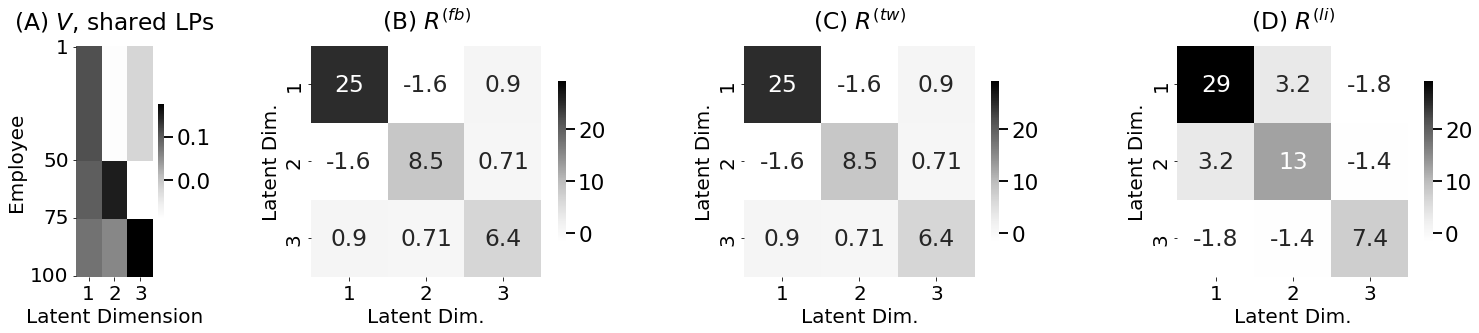
\includegraphics[width=\linewidth]{representations/ch5/Images/scores.png}
    \caption[Score matrices for COSIE model]{\textbf{(A)} the shared latent position matrix across all of the networks. \textbf{(B)} score matrix for the Facebook random network. \textbf{(C)} score matrix for the Twitter random network. \textbf{(D)} score matrix for the Linkedin random network.}
    \label{fig:ch5:scores}
\end{figure}

\subsubsection{Conceptualizing the COSIE model}

Finally, let's relate all of this back to the COSIE model. The way you can think about the COSIE model is that for each random network that you have, the probability matrix $P^{((m)}$ depends on the shared latent position matrix $V$ and the score matrix $R^{(m)}$. The probability matrix $P^{(m)}$ for the $m^{th}$ random network is defined so that $P^{(m)} = VR^{(m)}V^\top$. This means that each entry $p_{ij}^{(m)} = \vec v_i^\top R^{(m)} \vec v_j$. We say that a collection of random networks $\left\{\mathbf A^{(1)}, ..., \mathbf A^{(M)}\right\}$ with $n$ nodes is $COSIE_{n,M}\left(V, \left\{R^{(1)},...,R^{(M)}\right\}\right)$ if each random network $\mathbf A^{(m)}$ is $IER(P^{(m)})$. Stated another way, each of the $M$ random networks share the same orthonormal matrix $V$, but a unique score matrix $R^{(m)}$. This allows the random networks to share some underlying structure (which is conveyed by $V$) but each random network still has a combination of this shared structure (conveyed by $R^{(m)}$). 

Since the probability matrix $P^{(m)} = VR^{(m)}V^\top$, you can see that two random networks with the same score matrix will be homogeneous (identically distributed), and two random networks with different score matrices will be heterogeneous (not identically distributed). In this way, you are able to capture the homogeneity between the random networks for Facebook and Twitter connections, while also capturing the heterogeneity between the random networks for Facebook and Linkedin connections. The COSIE model is described by \cite{Arroyo2021}, and has direct connections with the multiple adjacency spectral embedding, which you will learn about in Section \ref{sec:ch6:multinet}.

\begin{floatingbox}[h]\caption{Check what you've learned}
To double check what you've learned so far, we would recommend that you play around with these results some. 

Demonstrate that you are able to recover the using the shared latent position matrices \texttt{V} and the score matrices \texttt{R\_facebook}, \texttt{R\_twitter}, and \texttt{R\_linkedin}. 

Show that the true probability matrices \texttt{P\_facebook\_twitter} and \texttt{P\_linkedin} are identical to the probability matrices that you obtain using the shared latent positions and the score matrices by using \texttt{np.allclose()}, like we did in Section \ref{sec:ch5:psd_block:lpm_fromsbm}.
\end{floatingbox}

\paragraph{Connections with the gRDPG}

The gRDPG random network, introduced briefly in Section \ref{sec:ch5:ier:grdpg}, is a little bit tough to conceptualize. To be precise, the initial formulation of the COSIE model in \cite{Arroyo2021} describes random networks which are gRDPGs (a broad class of models that is equivalent to IERs). To this end, the distinction is merely one of convenience for the audience: for expert statisticians who have built their careers in random network theory, the gRDPG may be more straightforward; to a broader audience, IER might be more straightforward. 

\subsection{Correlated Network Models}
\label{sec:ch5:multi:corr}

Finally, we get to a special case of network models, known as correlated network models. Let's say that you have a group of people in a city, and you know that each person in your group have both a Facebook and a Twitter account. The nodes in your network are the people who possess accounts. The first network consists of Facebook connections among the people, where an edge exists between two people if they are friends on Facebook. The second network consists of Twitter connections among the people, where an edge exists between two people if they follow one another on Twitter. You think that if two people are friends on Facebook, there is a good chance that they follow one another on Twitter, and vice versa. How do you reflect this similarity through a multiple network modelin which you can describe these ``correlations'' that arise?

At a high level, network correlation between a pair of networks describes the property that the existence of edges in one network provides you with some level of information about edges in the other network, much like the Facebook/Twitter example that you just saw. In this book, we will focus on the $\rho$-{correlated} network models ($\rho$ as in "rho", not "p"). What the $\rho$-correlated network models focus on is that given two random networks with the same number of nodes, each edge has a correlation of $\rho$ between the two networks. A pair of random networks $\mathbf A^{(1)}$ and $\mathbf A^{(2)}$ are called $\rho$-\textbf{correlated} if all of the edges across both networks are mutually independent, except that for all pairs of indices $i$ and $j$, $corr(\mathbf a_{ij}^{(1)}, \mathbf a_{ij}^{(2)}) = \rho$, where $corr(\mathbf x, \mathbf y)$ is the Pearson correlation between two random variables $\mathbf x$ and $\mathbf y$. In our example, this means that whether two people are friends on Facebook is {correlated} with whether they are following one another on Twitter.

The Pearson correlation describes whether one variable being large/small gives information that the other variable is large/small (positive correlation, between $0$ and $1$) or whether one variable being large/small gives information that the other variable will be small/large (negative correlation, between $-1$ and $0$). If the two networks are positively correlated and you know that one of the edges $\mathbf a_{ij}^{(1)}$ has a value of one, then you have information that $\mathbf a_{ij}^{(2)}$ might also be one, and vice-versa for taking values of zero. If the two networks are negatively correlated and you know that one of the edges $\mathbf a_{ij}^{(1)}$ has a value of one, then you have information that $\mathbf a_{ij}^{(2)}$ might be zero, and vice-versa. If the two networks are not correlated ($\rho = 0$) you do not learn anything about edges of network two by looking at edges from network one.

\subsubsection{$\rho$-Correlated RDPG}
\label{sec:ch5:multi:corr:rrdpg}

The $\rho$-correlated RDPG is the most general correlated network model you will need for the purposes of this book, and is described by \cite{Lyzinski2014Jan} and \cite{Pantazis2022}. Remembering that as ER, SBM, and DCSBM random networks are special cases of the RDPG (as long as the block matrix is positive semi-definite), the $\rho$-correlated RDPG can therefore be used to construct $\rho$-correlated ER, $\rho$-correlated SBMs, and $\rho$-correlated DCSBMs too. The way you can think about the $\rho$-correlated RDPG is that like for the normal RDPG, a latent position matrix $X$ with $n$ rows and a latent dimensionality of $d$ is used to define the edge-existence probabilities for the networks $\mathbf A^{(1)}$ and $\mathbf A^{(2)}$. The difference is that the probabilities in $\mathbf A^{(2)}$ now depend on the outcome of observing an instance of $\mathbf A^{(1)}$.

We begin by defining that $\mathbf A^{(1)}$ is $RDPG_n(X)$. Next, we define the second network as follows. We use a coin for each edge $(i, j)$, which has a probability that depends on the values that the first network takes. If the edge $\mathbf a_{ij}^{(1)}$ takes the value of one, then we use a coin which has a probability of landing on heads of $\vec x_i^\top \vec x_j + \rho(1 - \vec x_i^\top \vec x_j)$. If the edge $\mathbf a_{ij}^{(1)}$ takes the value of zero, then we use a coin which has a probability of landing on heads of $(1 - \rho)\vec x_i^\top \vec x_j$. We flip this coin, and if it lands on heads, then the edge $\mathbf a_{ij}^{(2)}$ takes the value of one. If it lands on tails, then the edge $\mathbf a_{ij}^{(2)}$ takes the value of zero. If $\mathbf A^{(1)}$ and $\mathbf A^{(2)}$ are random networks which are $\rho$-correlated RDPGs with latent position matrix $X$, we say that the pair $\left\{\mathbf A^{(1)}, \mathbf A^{(2)}\right\}$ are $\rho RDPG_n(X)$. 


\paragraph*{How do you simulate samples of $\rho RDPG_n(X)$ random networks?}

The procedure in Algorithm \ref{alg:ch5:rhordpg} will produce for you a pair of networks $A^{(1)}$ and $A^{(2)}$, which have nodes and edges, where the underlying random networks $\mathbf A^{(1)}$ and $\mathbf A^{(2)}$ are $\rho RDPG_n(X)$ random networks.

\begin{algorithm}[h]\caption{Simulating a paired sample of $\rho RDPG(X)$ random networks}
\label{alg:ch5:rhordpg}
\SetAlgoLined
\KwData{$n$ a number of nodes\newline $X$ a latent position matrix with $n$ rows and $d$ columns \newline $\rho$ a correlation between the two networks that is between $-1$ and $1$}
\KwResult{A pair of random networks which are $\rho$-correlated.}

Simulate a sample $A^{(1)}$ which is a sample  of an $RDPG_n(X)$ random network, using Algorithm \ref{alg:ch5:rdpg}.

\For{$i$ in $1$:$n$} {
    \For{$j > i$} {
        \If{$a_{ij}^{(1)} = 1$}{
            Obtain a coin which has a probability of landing on heads of $\vec x_i^\top \vec x_j + \rho(1 - \vec x_i^\top \vec x_j)$.
        } \Else {
            Obtain a coin which has a probability of landing on heads of $(1 - \rho)\vec x_i^\top \vec x_j$.
        }
        
        Flip the coin, and if it lands on heads, the corresponding entry $a_{ij}^{(2)}$ in the adjacency matrix is $1$. If the coin lands on tails, the corresponding entry $a_{ij}^{(2)}$ is $0$. 

        Set $a_{ji}^{(2)} = a_{ij}^{(2)}$.
    }
}

\Return{$A^{(1)}$ and $A^{(2)}$}

\end{algorithm}


Fortunately, \texttt{graspologic} makes sampling $\rho$-correlated RDPGs relatively simple. Let's take the same underlying model that we were working with above, and assert that the networks are not only identical in probability, but that they are also {correlated}. 

Conceptually, this is similar to asserting that if we knew that a pair of people were friends on Facebook, we might think that they would be more likely to be following one another on Twitter. We'll start by generating latent position matrices corresponding to the Twitter/Facebook example using code from Section \ref{sec:ch5:psd_block:lpm_fromsbm}:
\begin{lstlisting}[style=python]
from graphbook_code import lpm_from_sbm
X_facebook_twitter = lpm_from_sbm(z + 1, B)
\end{lstlisting}

Let's see what happens when the underlying correlation is $\rho = 0.7$. To summarize the differences between the two networks, we'll count the total number of edges that differ between the two networks, $\texttt{diff}\left(A^{(1)} - A^{(2)}\right)$:

\begin{lstlisting}[style=python]
from graspologic.simulations import rdpg_corr

# generate the network samples
rho = 0.7
facebook_correlated_network, twitter_correlated_network = rdpg_corr(
    X_facebook_twitter, Y=None, r=rho
)

# the difference matrix
correlated_difference_matrix = np.abs(
    facebook_correlated_network - twitter_correlated_network
)
# the total number of differences
correlated_differences = correlated_difference_matrix.sum()
\end{lstlisting}

A heatmap of the two networks is shown in Figure \ref{fig:ch5:rhordpg}(A) and Figure (B), along with the difference matrix in Figure \ref{fig:ch5:rhordpg}(C).

\begin{figure}
    \centering
    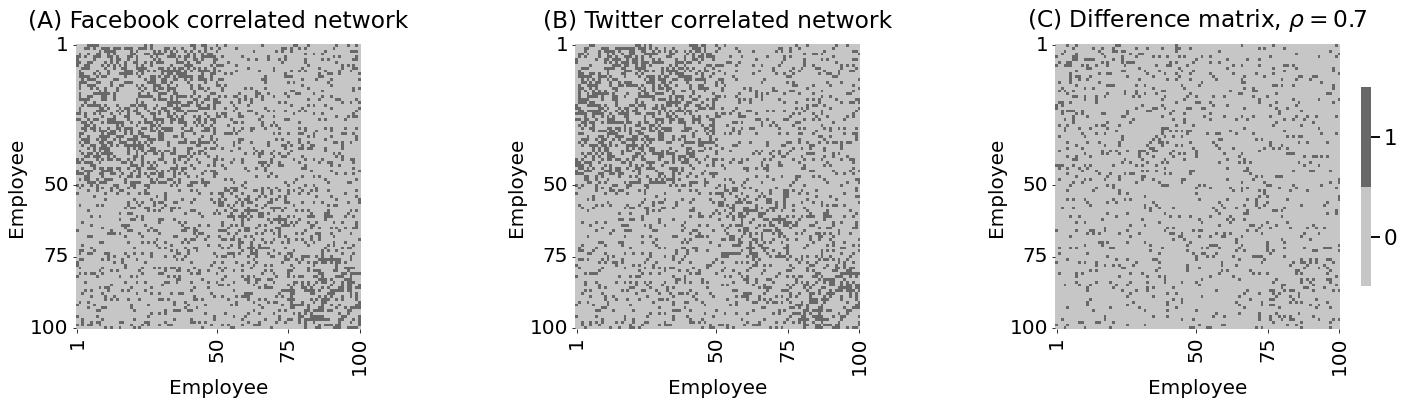
\includegraphics[width=\linewidth]{representations/ch5/Images/rhordpg.png}
    \caption[$\rho$-correlated RDPGs]{\textbf{(A)} the Facebook network. \textbf{(B)} the Twitter network. \textbf{(C)} the edges which differ between the two networks.}
    \label{fig:ch5:rhordpg}
\end{figure}
When the underlying correlation is much lower, such as $\rho' = 0.0$ (the networks are \textit{uncorrelated}), we can do the exact same thing:

\begin{lstlisting}[style=python]
rho_nil = 0.0
facebook_uncorrelated_network, twitter_uncorrelated_network = rdpg_corr(
    X_facebook_twitter, Y=None, r=rho_nil
)

# the difference matrix
uncorrelated_difference_matrix = np.abs(
    facebook_uncorrelated_network - twitter_uncorrelated_network
)
# the total number of differences
uncorrelated_differences = uncorrelated_difference_matrix.sum()
\end{lstlisting}

A heatmap of the two networks is shown in Figure \ref{fig:ch5:norhordpg}(A) and Figure (B), along with the difference matrix in Figure \ref{fig:ch5:norhordpg}(C). In both \ref{fig:ch5:rhordpg} and \ref{fig:ch5:norhordpg}, the Facebook and Twitter networks have {identical} latent position matrices, and the latent position matrices are the same for both scenarios. However, when the networks are correlated, the edges tend to be more similar between the two networks. When the networks are uncorrelated, the edges tend to differ more between the two networks. 

\begin{figure}[h]
    \centering
    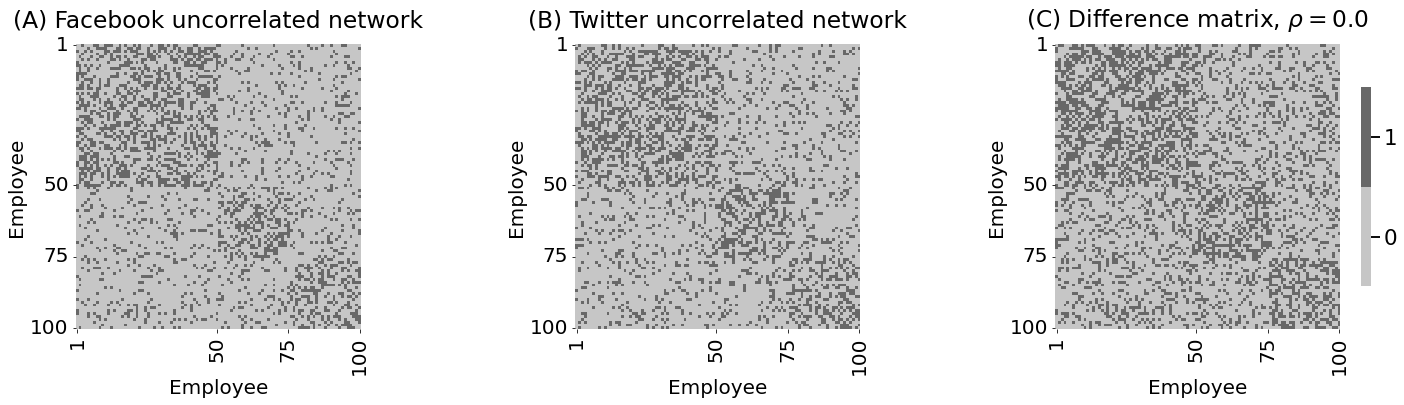
\includegraphics[width=\linewidth]{representations/ch5/Images/norhordpg.png}
    \caption[Uncorrelated RDPGs]{\textbf{(A)} the Facebook network. \textbf{(B)} the Twitter network. \textbf{(C)} the edges which differ between the two networks. Note that there are far more edges that differ than in Figure \ref{fig:ch5:rhordpg}.}
    \label{fig:ch5:norhordpg}
\end{figure}

\begin{floatingbox}[h]\caption{Negative $\rho$-correlated RDPGs}
If we generated another simulation where the networks were anti-correlated, we could arbitrarily increase the magnitude of this difference. Try the simulation again with $\rho$ as large as $-1$, and describe what you see. Repeat it a few times, and describe your result.

Next, do the simulation again with $\rho = 1.0$. What do you notice?
\end{floatingbox}

\newpage
\section{Models with Covariates}
\label{sec:ch5:multicovar}


To conclude your learnings on network models, we're going to delve into a common problem in machine learning known as the classification problem. For each piece of data $x_i$ in your sample, you might often have another piece of information $y_i$ associated with this data which you think is associated with the data $x_i$ in some way. This additional information $y_i$ is known as the \textbf{class} of the $i^{th}$ item, and is a \textit{categorical variable} which takes values between $1$ and $Y$, where $Y$ is the total number of possible classes in your experiment. A \textbf{categorical variable} is a variable that can take one of a fixed set of possible values. Consider the case where you have the heights of a selection of people and aliens for a hypothetical sample. The data $x_i$ is the height of each individual $i$. $y_i$ indicates whether the $i^{th}$ individual is a person (1) or an alien (2). $y_i$ is a categorical variable because you chose people to be $1$ and aliens to be $2$ arbitrarily, and the total number of classes $Y$ is $2$. Your question of interest is the extent to which you can \textit{predict} the class for each individual (person or alien) using only their height $x_i$. 

Now let's imagine that you have a collection of networks representing the brains of $100$ individuals $500,000$ years into the future (let's hope humanity makes it that long!). These individuals are all either humans who have persisted with life-as-normal on earth (earthlings), or astronauts who left for a planet with a different set of prominent colors and light content from Earth. The environment was extremely harsh, so there were evolutionary pressures on your astronauts towards people whose eyes could better adapt to the different set of colors and light on the new planet. 

Each network has $5$ nodes, representing the sensory functions and modalities of the brain: the area responsible for sight (S), the area responsible for language (L), the area responsible for hearing/emotional expression (H/E), the area responsible for thinking/movement (T/M), and the area responsible for basic survival functions (such as heartbeat and breathing, MS). Edges represent whether pairs of brain areas can pass information to one another. In this case, you have observed pairs of data $(A^{(m)}, y_m)$, for $m$ from $1$ to $M=100$. Each adjacency matrix $A^{(m)}$ is a $5 \times 5$ matrix, and the indicator variable $y_m$ takes the value $1$ if the $m^{th}$ individual is an earthling, or $2$ if the $m^{th}$ individual is an astronaut. In this case, you want to predict the class for each individual (earthling or astronaut) using only their adjacency matrix $A^{(m)}$. You can see two example networks for the earthlings and the astronauts below:

\begin{lstlisting}[style=python]
from graspologic.simulations import sample_edges
import numpy as np
from graphbook_code import heatmap

n = 5
P_hum = np.random.beta(size=n*n, a=3, b=8).reshape(n, n)
# networks are undirected, so symmetrize the probability matrix
P_hum = (P_hum + P_hum.T)/2

# networks are simple, so undirected
P_hum = P_hum - np.diag(np.diag(P_hum))

nodenames = ["Sight", "Language", "Hearing/\nEmotion", "Thinking/\nMovement", "Basic \nSurvival"]
ssn = np.zeros((n, n))
ssn[1:n,:] = 1
ssn[:,1:n] = 1
P_ast = np.copy(P_hum)

# probabilities for signal edges are higher in astronauts than humans
P_ast[ssn] = np.sqrt(P_ast[ssn])

Ahum = sample_edges(P_hum)
Aast = sample_edges(P_ast)
\end{lstlisting}

A plot which compares the two adjacency matrices is shown in Figure \ref{fig:ch5:ssg_samps}. Just looking at these two matrices, it's a little bit unclear how we can derive meaningful information about this problem, particularly with respect to the edges in the first column and the first row (corresponding to the node that we \textit{said} was different, the node responsible for ``sight''). Is there some way that we could ``pool'' across the networks, and see if perhaps we could gain insight by thinking about a property shared by all of the networks from a single class (astronaut vs. earthling)?

\begin{figure}
    \centering
    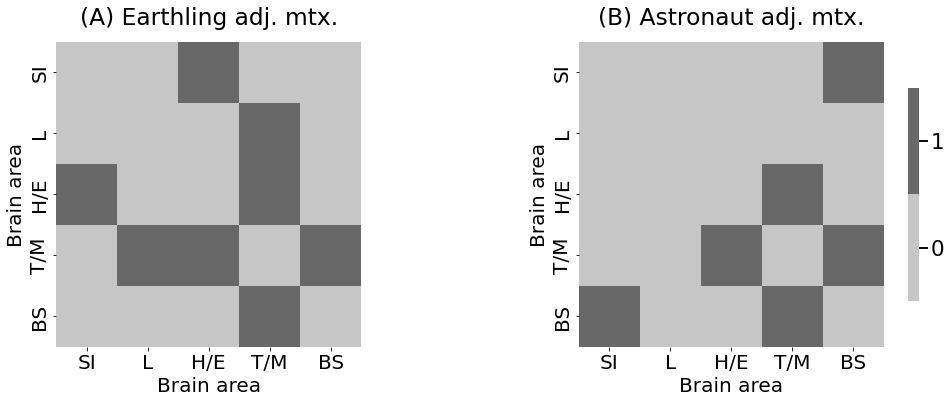
\includegraphics[width=0.7\linewidth]{representations/ch5/Images/ssg_samps.png}
    \caption[Two samples of adjacency matrices from the signal sub network model]{\textbf{(A)} a brain network of an earthling. \textbf{(B)} a brain network of an astronaut.}
    \label{fig:ch5:ssg_samps}
\end{figure}

Remember that to devise a statistical model, you suppose each piece of data in your sample is an observation of a corresponding random variable. When you were dealing with multiple network models, this meant that for each network $A^{(m)}$ there was a random network $\mathbf A^{(m)}$, and that this random network was the data-generating process that we were observing $A^{(m)}$ from. Here, for each data pair $(A^{(m)}, y_m)$, there exists a corresponding random network $\mathbf A^{(m)}$ and a corresponding random class $\mathbf y_m$, where $(A^{(m)}, y_m)$ is a sample of $(\mathbf A^{(m)}, \mathbf y_m)$. So, for your multiple network model with covariates, you seek a model which describes both $\mathbf A^{(m)}$ and $\mathbf y_m$.
\subsection{Signal Subnetwork Model}

As it turns out, these astronauts are remarkably similar to the eathlings, except for one piece of information: the connections between the occipital lobe and all other lobes for the astronauts have a much higher chance of being connected. In other words, the \textit{subnetwork} comprised of edges incident the occipital lobe carry the \textit{signal disparity} between human and astronaut brains. This concept of a subnetwork was first explored in Section \ref{sec:ch4:prop-net:subnetwork}. 

What this means is that, if you were to just compare the adjacency matrices themselves, you would end up looking at a lot of \textit{noise}, or edges which do not show any difference between the humans and the astronauts. In a fixed sample of earthlings and astronauts, you might find disparities between these noise edges, but these disparities are just because of the particular sample of humans and astronauts that you chose and are not representative of actual differences. Rather, what you want to do is identify the subset of edges and corresponding nodes, called the \textit{signal subnetwork}, which actually carry the \textit{signal}, the set of edges which show real differences between the earthlings and the astronauts. Below, we plot the probability matrices for earthlings and astronauts:

\begin{lstlisting}[style=python]
# plot prob. mtxs and the difference on same scale
heatmap(P_hum, vmin=0, vmax=1)
heatmap(P_ast, vmin=0, vmax=1)
heatmap(P_hum - P_ast, vmin=0, vmax=1)
\end{lstlisting}

Which we examine in detail in Figure \ref{fig:ch5:ssg_pmtxs}. Notice that the \textit{entirety} of the disparity between earthlings and astronauts (in terms of their probability matrices) shown in Figure \ref{fig:ch5:ssg_ssn}(C) is captured by the edges which include a node involved in eyesight. You can observe this because the first row and column of the matrix (corresponding to the node for eyesight) is different between the two networks for all other pairs of nodes.

\begin{figure}
    \centering
    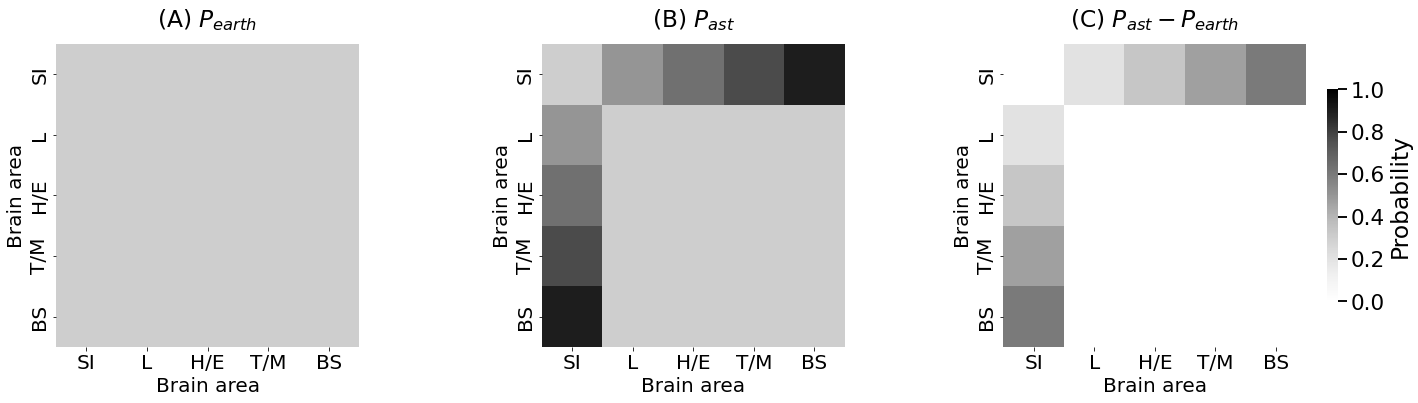
\includegraphics[width=\linewidth]{representations/ch5/Images/ssg_pmtxs.png}
    \caption[Probability matrices from two different classes]{\textbf{(A)} the probability matrix for brain networks of earthlings. \textbf{(B)} the probability matrix for brain networks of astronauts. \textbf{(C)} the difference between the probability matrices for astronauts and humans. Notice that the the area responsible for sight, SI, has very different connection probabilities with all other brain areas.}
    \label{fig:ch5:ssg_pmtxs}
\end{figure}

We will attempt to do this using the \textit{signal subnetwork model}, which is a statistical model for adjacency matrices where you have a covariate. When you want to later decide whether a network is from an earthling or an astronaut, you want to look \textit{only} at the signal subnetwork, and ignore the rest of the network entirely.

For the SSN model, the core idea is that for each edge in the network, the probability of an edge existing (or not existing) is either the same, or different, between the two classes. You capture this idea using the \textbf{signal subnetwork}. For an edge $(i, j)$ for classes $y$ (either $0$ or $1$), you will use the notation $p_{ij}^y$ to denote the probability of an edge existing in class $y$. 

\subsubsection{Signal Subnetwork}

The \textbf{signal subnetwork} \cite{Vogelstein2013Jul} is a collection of edges $\mathcal S$, which has edges $(i,j)$ where $i$ and $j$ are nodes in the network between $1$ and $n$, such that the following two conditions hold:

\begin{enumerate}
    \item For each edge which is in the signal subnetwork, the probability of an edge existing differs between classes $0$ and $1$. That is, if an edge $(i, j)$ is in the signal subnetwork $\mathcal S$, then there exist two classes $y$ and $y'$ where $p_{ij}^{y} \neq p_{ij}^{y'}$.
    \item For each edge which is \textit{not} in the signal subnetwork, the probabilitty of an edge existing is the \textit{same} between classes $0$ and $1$. That is, if an edge $(i, j)$ is not in the signal subnetwork $\mathcal S$, then $p_{ij}^0 = p_{ij}^1$. For this reason, if an edge is not in the signal subnetwork, you will use the term $p_{ij} = p_{ij}^0 = p_{ij}^1 = ... = p_{ij}^Y$.
\end{enumerate}

This sounds a little complex, but it's really quite simple: the idea is just that the signal subnetwork is keeping track of the edges which have different probabilities for any pair of classes. For your earthlings versus astronauts example above, this amounts to the set of edges for which at least one node is the occipital lobe:

\begin{lstlisting}[style=python]
# plot the signal subnetwork
ax = heatmap(ssn.astype(int))
\end{lstlisting}

\begin{figure}
    \centering
    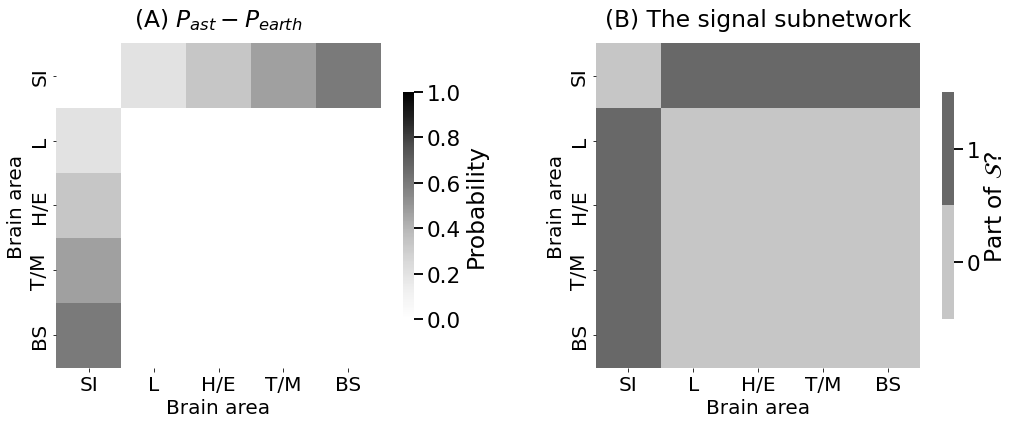
\includegraphics[width=\linewidth]{representations/ch5/Images/ssg_ssn.png}
    \caption[Signal subnetwork for earthling and astronaut examples]{\textbf{(A)} the difference between the earthling and astronaut probability matrices. \textbf{(B)} the signal subnetwork.}
    \label{fig:ch5:ssg_ssn}
\end{figure}

A plot of the signal subnetwork is shown in Figure \ref{fig:ch5:ssg_ssn}(B), and is compared to the difference between the probability matrices for earthlings and astronauts in Figure \ref{fig:ch5:ssg_ssn}(A). Notice that the signal subnetwork includes \textit{all} edges in which the two probability matrices are different. 

Now that we are familiar with the signal subnetwork $\mathcal S$, we can formally define the signal subnetwork model. For each random pair $(\mathbf A^{(m)}, y_m)$ of your $M$ total pairs, you first obtain a ``class assignment'' die with $Y$ total sides. For a given face of the dice $y$, the probability that the dice lands on side $Y$ is $\pi_y$. You flip the class assignment die, and if it lands on side $y$, then $\mathbf y_m$ takes the value $y$. Next, for each edge $(i,j)$ which is not in the signal subnetwork $\mathcal S$, you obtain a ``non-signal’’ coin which has a probability of $p_{ij}$ of landing on heads and $1 - p_{ij}$ of landing on tails. The edge $\mathbf a_{ij}$ exists if the coin lands on heads and does not exist if the coin lands on tails. Finally, for each edge $(i, j)$ which is in the signal subnetwork $\mathcal S$, you check which class $\mathbf y_m$ indicates. If $\mathbf y_m$ is class $y$, you obtain a ``signal’’ coin which has a probability of $p_{ij}^y$ of landing on heads, and a probability of $1 - p_{ij}^y$ of landing on tails. The edge $\mathbf a_{ij}$ exists if the coin lands on heads and does not exist if the coin lands on tails. In summary, say that a collection of random network/covariate pairs $\left\{(\mathbf A^{(1)}, \mathbf y_1), ..., (\mathbf A^{(M)}, \mathbf y_M)\right\}$ with $n$ nodes is $SSN_n(\pi_1, ..., \pi_Y, P^1, ..., P^Y, \mathcal S)$ if the following three conditions hold:
1. For every edge $(i, j)$ which is in the signal subnetwork $\mathcal S$, then there exist at least two classes $y$ and $y'$ where $p_{ij}^y \neq p_{ij}^{y'}$.
2. For every edge $(i, j)$ which is not in the signal subnetwork $\mathcal S$, then every edge probability $p_{ij}=p_{ij}^1 =...= p_{ij}^Y$. 
3. conditional on the class $\mathbf y_m$ being $y$, then $\mathbf A^{(m)}$ is $IER_n(P^y)$, where $IER_n(P^y)$ is from Section \ref{sec:ch5:ier}.

Next, let's learn how to simulate signal subnetworks.
\subsection{How do you simulate samples of $SSN_n(\pi_1, ..., \pi_Y, P^1, ..., P^Y, \mathcal S)$ random networks?}

The procedure below in Algorithm \ref{alg:ch5:ssn} produce for you a set of networks, $A^{(1)}, ..., A^{(M)}$, which have nodes and edges, where the underlying random networks $\left\{\mathbf A^{(1)},..., \mathbf A^{(M)}\right\}$ are $SSN_{n,M}(\pi_1,..., \pi_Y, P^1,..., P^Y, \mathcal S)$ random networks.


\begin{algorithm}[h]\caption{Simulating a sample from an $SSN_{n, M}(\pi_1, ..., \pi_Y, P^1, ..., P^Y, \mathcal S)$ random network}
\label{alg:ch5:ssn}
\SetAlgoLined
\KwData{$n$ a number of nodes\newline $M$ the total number of networks \newline $\pi_1,..., \pi_Y$ the probability of a network being from a given class \newline $P^1, ..., P^Y$ the probability matrix associated with each class \newline $\mathcal S$ the signal subnetwork}
\KwResult{A collection of $M$ networks with $n$ nodes.}

Obtain a dice with $Y$ sides, that has a $\pi_y$ chance of landing on the $y$ side.

\For{$m$ in $1$:$M$} {
    Flip the $Y$-sided die, and if it lands on side $y$, assign the item $m$ to class $y$.

    Simulate an adjacency matrix $A^{(m)}$, using the procedure for an $IER_n(P^{(y)})$ network, in Algorithm \ref{alg:ch5:ier}.
}

\Return{$\left\{A^{(1)},...,A^{(M)}\right\}$}
\end{algorithm}


\bibliographystyle{vancouver}
\bibliography{references}